% !TEX encoding = UTF-8 Unicode
%
%
% UCSD Doctoral Dissertation Template
% -----------------------------------
% http://ucsd-thesis.googlecode.com
%
%
% ----------------------------------------------------------------------
% WARNING: 
%
%   This template has not endorced by OGS or any other official entity.
%   The official formatting guide can be obtained from OGS.
%   It can be found on the web here:
%   http://ogs.ucsd.edu/AcademicAffairs/Documents/Dissertations_Theses_Formatting_Manual.pdf
%
%   No guaranty is made that this LaTeX class conforms to the official UCSD guidelines.
%   Make sure that you check the final document against the Formatting Manual.
%  
%   That being said, this class has been routinely used for successful 
%   publication of doctoral theses.  
%
%   The ucsd.cls class files are only valid for doctoral dissertations.
%
%
% ----------------------------------------------------------------------
% GETTING STARTED:
%
%   Lots of information can be found on the project wiki:
%   http://code.google.com/p/ucsd-thesis/wiki/GettingStarted
%
%
%   To make a pdf from this template use the command:
%     pdflatex template
%
%
%   To get started please read the comments in this template file 
%   and make changes as appropriate.
%
%   If you successfully submit a thesis with this package please let us
%   know.
%
%
% ----------------------------------------------------------------------
% KNOWN ISSUES:
%
%   Currently only the 12pt size conforms to the UCSD requirements.
%   The 10pt and 11pt options make the footnote fonts too small.
%
%
% ----------------------------------------------------------------------
% HELP/CONTACT:
%
%   If you need help try the ucsd-thesis google group:
%   http://groups.google.com/group/ucsd-thesis
%
%
% ----------------------------------------------------------------------
% BUGS:
%
%   Please report all bugs at:
%   http://code.google.com/p/ucsd-thesis/issues/list
%
%
% ----------------------------------------------------------------------
% More control of the formatting of your thesis can be achieved through
% modifications of the included LaTeX class files:
%
%   * ucsd.cls    -- Class file
%   * uct10.clo   -- Configuration files for font sizes 10pt, 11pt, 12pt
%     uct11.clo                            
%     uct12.clo
%
% ----------------------------------------------------------------------



% Setup the documentclass 
% default options: 12pt, oneside, final
%
% fonts: 10pt, 11pt, 12pt -- are valid for UCSD dissertations.
% sides: oneside, twoside -- note that two-sided theses are not accepted 
%                            by OGS.
% mode: draft, final      -- draft mode switches to single spacing, 
%                            removes hyperlinks, and places a black box
%                            at every overfull hbox (check these before
%                            submission).
% chapterheads            -- Include this if you want your chapters to read:
%                              Chapter 1
%                              Title of Chapter
%
%                            instead of
%                              1 Title of Chapter
\documentclass[12pt,chapterheads]{ucsd}
% \documentclass[12pt,chapterheads]{ucsd}

% Include all packages you need here.  
% Some standard options are suggested below.
%
% See the project wiki for information on how to use 
% these packages. Other useful packages are also listed there.
%
%   http://code.google.com/p/ucsd-thesis/wiki/GettingStarted

% Compile without creating PDF output to speed up error checking
% \usepackage{syntonly}
% \syntaxonly

%% AMS PACKAGES - Chances are you will want some or all 
%    of these if writing a dissertation that includes equations.
%  \usepackage{amsmath, amscd, amssymb, amsthm}
\usepackage{amsmath,bm}

%% GRAPHICX - This is the standard package for 
%    including graphics for latex/pdflatex.
\usepackage{scrextend}
\usepackage{pslatex}
\usepackage{graphicx}

\usepackage{subfig}
\usepackage{floatrow}
\floatsetup[table]{capposition=above,captionskip=-10pt}


%\usepackage{subcaption}
\usepackage{xcolor}
\usepackage{adjustbox}
\usepackage{verbatim}
\usepackage{amssymb}
%% CAPTION
% This overrides some of the ugliness in ucsd.cls and
% allows the text to be double-spaced while letting figures,
% tables, and footnotes to be single-spaced--all OGS requirements.
% NOTE: Must appear after graphics and ams math
\makeatletter
\gdef\@ptsize{2}% 12pt documents
\let\@currsize\normalsize
\makeatother
\usepackage{setspace}
\doublespace
\usepackage[font=small, width=0.9\textwidth]{caption}

\usepackage{longtable}

\usepackage[T1]{fontenc}
\usepackage[utf8]{inputenc}
\usepackage[english]{minitoc}

%% CITATIONS
% break long URLs

\usepackage[
url=false,
doi=false,
alldates=year,  % in case citation includes month
% urldate=short,
refsegment=chapter,
maxcitenames=2,
maxbibnames=200,
backend=biber,
style=authoryear,
uniquename=false,
uniquelist=false,
%citestyle=authoryearbracket,
giveninits=true,
natbib=true,
]{biblatex}

\DefineBibliographyStrings{english}{%
  andothers = {\textit{et al}\adddot}
}

\DeclareNameAlias{author}{family-given}
\renewcommand{\postnotedelim}{\addsemicolon\addspace}
\addbibresource{references.bib}
%\bibliographystyle{apalike}

%\usepackage[backref=true,refsection=chapter]{biblatex}
% Break on URL numbers if too wide
\usepackage{xurl}
\def\UrlBreaks{\do\/\do-}
\setcounter{biburllcpenalty}{8000}
\setcounter{biburlucpenalty}{8000}
\setcounter{biburlnumpenalty}{8000}


% Sets citation format
% and fixes up citations madness
\usepackage{microtype}  % avoids citations that hang into the margin

% Other helpful snippets
% citep with leading "e.g., " 
\newcommand{\citeg}[1]{\citep[e.g.,][]{#1}}
% Write short author before author, useful for institutions with abbreviation.
\renewbibmacro*{begentry}{%
    \ifnameundef{shortauthor}
        {}
        {\printnames{shortauthor}%
         \addspace\textendash\space}}

%% SUBFIG - Use this to place multiple images in a
%    single figure.  Subfig will handle placement and
%    proper captioning (e.g. Figure 1.2(a))
% \usepackage{subfig}

%% TIMES FONT - replacements for Computer Modern
%%   This package will replace the default font with a
%%   Times-Roman font with math support.
% \usepackage[T1]{fontenc}
% \usepackage{mathptmx}

%% INDEX
%   Uncomment the following two lines to create an index: 
% \usepackage{makeidx}
% \makeindex
%   You will need to uncomment the \printindex line near the
%   bibliography to display the index.  Use the command
% \index{keyword} 
%   within the text to create an entry in the index for keyword.
%   To compile a LaTeX document with an index the 'makeindex'
%   command will need to be run.  See the wiki for more details.

%% HYPERLINKS
%   To create a PDF with hyperlinks, you need to include the hyperref package.
%   THIS HAS TO BE THE LAST PACKAGE INCLUDED!
%   Note that the options plainpages=false and pdfpagelabels exist
%   to fix indexing associated with having both (ii) and (2) as pages.
%   Also, all links must be black according to OGS.
%   See: http://www.tex.ac.uk/cgi-bin/texfaq2html?label=hyperdupdest
%   Note: This may not work correctly with all DVI viewers (i.e. Yap breaks).
%   NOTE: hyperref will NOT work in draft mode, as noted above.
% \usepackage[colorlinks=true, pdfstartview=FitV, 
%             linkcolor=black, citecolor=black, 
%             urlcolor=black, plainpages=false,
%             pdfpagelabels]{hyperref}
% \hypersetup{ pdfauthor = {Your Name Here}, 
%              pdftitle = {The Title of The Dissertation}, 
%              pdfkeywords = {Keywords for Searching}, 
%              pdfcreator = {pdfLaTeX with hyperref package}, 
%              pdfproducer = {pdfLaTeX} }
% \urlstyle{same}
% \usepackage{bookmark}
%\usepackage{CJKutf8}



%% FOOTNOTE-MAGIC
% Enables footnotes in tables, re-referencing the same footnote multiple times.
\usepackage{footnote}
\makesavenoteenv{tabular}
\makesavenoteenv{table}


%% TABLE FORMATTING MADNESS
% Enable all sorts of fun table tricks
\usepackage{rotating}  % Enables the sideways environment (NCPW)
\usepackage{array}  % Enables "m" tabular environment http://ctan.org/pkg/array
\usepackage{booktabs}  % Enables \toprule  http://ctan.org/pkg/array
\usepackage{multirow}
\usepackage{threeparttable}
\setlength\bibitemsep{2\itemsep}

%\urlstyle{same}
\usepackage[breaklinks,pdfencoding=auto,psdextra]{hyperref}
\PassOptionsToPackage{unicode}{hyperref}
\hypersetup{
    colorlinks,
    linkcolor={black},
    citecolor={black},
    urlcolor={black}
}
\usepackage[capitalize]{cleveref}

\begin{document}
\captionsetup{justification=justified,singlelinecheck=false}
%\begin{comment}
%% FRONT MATTER
%
%  All of the front matter.
%  This includes the title, degree, dedication, vita, abstract, etc..
%  Modify the file template_frontmatter.tex to change these pages.
%
%
% UCSD Doctoral Dissertation Template
% -----------------------------------
% http://ucsd-thesis.googlecode.com
%
%


%% REQUIRED FIELDS -- Replace with the values appropriate to you

% No symbols, formulas, superscripts, or Greek letters are allowed
% in your title.
\title{Toward high-frequency deterministic simulations: source, path and site effects}

\author{Zhifeng Hu}
\degreeyear{\the\year}

% Master's Degree theses will NOT be formatted properly with this file.
\degreetitle{Doctor of Philosophy}

\field{Geophysics}
%\specialization{Anthropogeny}  % If you have a specialization, add it here

\chair{Kim Olsen}
% Uncomment the next line iff you have a Co-Chair
%\cochair{Professor }
%
%
% Or, uncomment the next line iff you have two equal Co-Chairs.
%\cochairs{Professor Chair Masterish}{Professor Chair Masterish}

%  The rest of the committee members  must be alphabetized by last name.
\othermembersucsd{
    \hspace*{0.5in} Joel Conte\\
    \hspace*{0.5in} Peter Shearer\\
}

\othermemberssdsu{
    \hspace*{0.5in} Steven Day\\
    \hspace*{0.5in} Daniel Roten\\
    \hspace*{0.5in} Samuel Shen\\
}
\numberofmembers{6} % |chair| + |cochair| + |othermembers|
\urlstyle{same}

%% START THE FRONTMATTER
%
\begin{frontmatter}

    %% TITLE PAGES
    %
    %  This command generates the title, copyright, and signature pages.
    %
    \makefrontmatter

    %% DEDICATION
    %
    %  You have three choices here:
    %    1. Use the ``dedication'' environment.
    %       Put in the text you want, and everything will be formated for
    %       you. You'll get a perfectly respectable dedication page.
    %
    %
    %    2. Use the ``mydedication'' environment.  If you don't like the
    %       formatting of option 1, use this environment and format things
    %       however you wish.
    %
    %    3. If you don't want a dedication, it's not required.
    %
    %
    \begin{dedication}
        \vspace*{\fill}
        To my family \par Xiaoyang, Xiuhong and Fei \par
        \vspace*{\fill}
    \end{dedication}


    % \begin{mydedication} % You are responsible for formatting here.
    %   \vspace{1in}
    %   \begin{flushleft}
    % 	To me.
    %   \end{flushleft}
    %
    %   \vspace{2in}
    %   \begin{center}
    % 	And you.
    %   \end{center}
    %
    %   \vspace{2in}
    %   \begin{flushright}
    % 	Which equals us.
    %   \end{flushright}
    % \end{mydedication}



    %% EPIGRAPH
    %
    %  The same choices that applied to the dedication apply here.
    %
    \begin{epigraph} % The style file will position the text for you.

        \emph{
            You must know that a person’s ability to discern the truth \\
            is directly proportional to his knowledge.
        }\\
        --- Cixin Liu, The Three-Body Problem \par

        \setlength{\parskip}{40pt plus 1pt minus 1pt}
        \emph{There are only the pursued, the pursuing, the busy and the tired.}\\
        --- F. Scott Fitzgerald, The Great Gatsby \par

        \setlength{\parskip}{40pt plus 1pt minus 1pt}
        \emph{Never confuse education with intelligence, \\
            you can have a PhD and still be an idiot.}\\
        --- Richard P. Feynman \par


    \end{epigraph}

    % \begin{myepigraph} % You position the text yourself.
    %   \vfil
    %   \begin{center}
    %     {\bf Think! It ain't illegal yet.}
    %
    % 	\emph{---George Clinton}
    %   \end{center}
    % \end{myepigraph}


    %% SETUP THE TABLE OF CONTENTS
    %
    \tableofcontents
    \listoffigures  % Comment if you don't have any figures
    \listoftables   % Comment if you don't have any tables



    %% ACKNOWLEDGEMENTS
    %
    %  While technically optional, you probably have someone to thank.
    %  Also, a paragraph acknowledging all coauthors and publishers (if
    %  you have any) is required in the acknowledgements page and as the
    %  last paragraph of text at the end of each respective chapter. See
    %  the OGS Formatting Manual for more information.
    %
    \begin{acknowledgements}

        % I have always been recalling the time I walked along the La Jolla beach years ago, when the afterglow of sunset lingered forever, and the path ahead extended beyond the sight of my eyes. It came to me that the time paused, and I could repeat those days once and once again, which, I do not know when, fades out and now the end of this journey arrives. Fortunately, I have been accompanied by the greatest people, to whom I owe my sincere appreciation.

        First and foremost, I would like to express my deepest sense of gratitude to my supervisor, Professor Kim Olsen, for his invaluable supervision, support, and tutelage during the course of my PhD studies. Kim always gives me the freedom to explore problems, allows me to try different approaches, and re-directs me every time I move in a wrong direction. He is always responsive to asking and patient to answering, even if my questions are naive. His suggestions and comments are so detailed and constructive that they easily refresh my thoughts and guide me in the right direction. I am always impressed by his skills in applying physical sense in solving problems and providing relevant knowledge in a timely manner. He emphasizes the big picture in seismology, while at the same time taught me how to present scientific findings, polish academic reports and communicate with the community. I appreciate the wealth of knowledge he has given me.

        It is my privilege to thank my committee members for their great mentorship and guidance. I thank Professor Steve Day, who is always supportive and encouraging. Even during the most difficult times, I feel encouraged thinking of his optimistic attitude and enthusiasm in life. He is rigorous to scientific problems but open to explore different possibilities, to which he always provides valuable comments and insights. It was an honor to attend his retirement ceremony in person and see how a life of contribution to science is remembered and respected. Professor Peter Shearer is the person leading me to this field by his popular course "Introduction to Seismology", which is still an important source of answers in my research. He showed me that science can be elegant yet fun. I thank Professor Samuel Shen for his valuable help in mathematics in our discussions. I also thank Professor Joel Conte for his kind suggestions and comments. Dr. Daniel Roten is extraordinarily supportive in Kim's group, who taught me the details in research practice from the beginning. I cannot overstate how much I learned from him, and it is my privilege to work with someone as versatile, brilliant, and productive as Daniel. I am also grateful to Professor Shuo Ma at SDSU for sharing his experience and life advice.

        I am grateful to all the professors at Scripps Institution of Oceanography (SIO) and SDSU, who taught a wide series of courses that prepared me for my research, including Professor Duncan Agnew, Professor Adrian Borsa, Professor Catherine Constable, Professor Steven Constable, Professor Yuri Fialko, Professor Guy Masters, Professor David Sandwell, Professor Peter Shearer, and Professor Dave Stegman at Scripps Institution of Oceanography at UCSD; Professor Michael Holst in the Department of Mathematics at UCSD; and Professor Shuo Ma and Professor Kim Olsen at SDSU.

        My research achievements would not be possible without the help and communication from my coauthors and collaborators from the Southern California Earthquake Center. I thank Kim Olsen, Steven Day, Daniel Roten, Christine Goulet, Robert Graves, Fabio Silva, Scott Callaghan, and Kevin Milner for their incredible collaborations and discussions.

        I appreciate the support and friendship from my incredible fellows and friends: Nan Wang, Te-Yang Yeh, Yongfei Wang, Shiying Nie, Qian Yao, Wei Wang, Zefeng Li, Yuxiang Zhang, Bill Savran, Kyle Withers, Drake Singleton, Rumi Takedatsu, Xiaohua Xu, Kang Wang, Wenyuan Fan, Zhao Chen, Yuval Levy, Zeyu Jin, Yue Du, Zheng Fang, Junlong Hou, Mingda Li, and Yuan Huang. Thank you for making my time at San Diego a wonderful memory. I also appreciate the administrative advisors and staff, including Gilbert Bretado, Wayne Farquharson, Paul Dean, and Sara Miceli at UCSD; Irene Occhiello, Pia Parrish, Heather Webb, Susan Langsford, and Pat Walls at SDSU, for their consistent and timely assistance.

        Finally, I would also like to extend my deepest gratitude to my parents, Xiaoyang and Xiuhong, for always listening to me, supporting me, and encouraging me. Lastly but most importantly, I thank Fei for being there for me, for always believing in me, and for enriching my life in numerous amounts of ways.

        \bigskip


        \Cref{chap:vs30}, in full, is a reformatted version of a paper currently being prepared for submission for publication: Hu, Z., Olsen, K.B., and Day S.M. (2021). Calibration of the Near-surface Seismic Structure in the SCEC Community Velocity Model Version 4.
        The dissertation author was the primary investigator and author of this paper.

        \Cref{chap:highf}, in full, is a reformatted version of a paper currently in preparation for submission for publication: Hu, Z., Olsen, K.B. and Day, S.M. (2021), 0-5 Hz Deterministic 3D Ground Motion Simulations for the 2014 La Habra, California, Earthquake. The dissertation author was the primary investigator and author of this paper.

        \Cref{chap:etf}, in full, is a reformatted version of the material as it appears in Bulletin of the Seismological Society of America: Hu, Z., Roten, D., Olsen, K.B. and Day, S.M. (2020). Modeling of Empirical Transfer Functions with 3D Velocity Structure. \emph{Bulletin of the Seismological Society of America}. The dissertation author was the primary investigator and author of this paper.

        \Cref{chap:eks}, in full, is a reformatted version of a report to the Southern California Earthquake Center: Hu, Z., Roten, D., Olsen, K.B., and Day, S.M. (2021). Kinematic Source Models for Earthquake Simulations with Fault-zone Plasticity. The dissertation author was the primary investigator and author of this manuscript.


    \end{acknowledgements}


    %% VITA
    %
    %  A brief vita is required in a doctoral thesis. See the OGS
    %  Formatting Manual for more information.
    %
    \begin{vitapage}
        \begin{vita}
            \item[2015] B.S. in Geophysics, Peking University
            \item[2015-2021] Graduate Teaching/Research Assistant, San Diego State University
            \item[2021] Ph.D. in Geophysics, University of California, San Diego and San Diego State University
        \end{vita}
        \begin{publications}
            \item \textbf{Hu, Z.}, Roten, D., Olsen, K.B., and Day, S.M. (2021) Kinematic Source Models for Earthquake Simulations with Fault-zone Plasticity. \emph{In preparation for publication}.
            \item \textbf{Hu, Z.} and Olsen, K.B. (2021). 0-5 Hz Deterministic 3D Ground Motion Simulations for the 2014 La Habra, California, Earthquake. \emph{To be submitted for publication}.
            \item \textbf{Hu, Z.}, Olsen, K.B., and Day, S.M. (2021). Calibration of the Near-surface Seismic Structure in the SCEC Community Velocity Model Version 4. \emph{To be submitted for publication}.
            \item O'Reilly O., Yeh, T. Olsen, K.B., \textbf{Hu, Z.}, Breuer, A.N., Roten D., Goulet C. (2021). A High-order Finite Difference Method on Staggered Curvilinear Grids for Seismic Wave Propagation Applications with Topography, \emph{Bulletin of the Seismological Society of America}. \emph{Accepted for publication, June 10, 2021}.
            \item \textbf{Hu, Z.}, Roten, D., Olsen, K.B., and Day, S.M. (2020). Modeling of Empirical Transfer Functions with 3D Velocity Structure. \emph{Bulletin of the Seismological Society of America}. \url{doi:10.1785/0120200214}.


        \end{publications}
    \end{vitapage}


    %% ABSTRACT
    %
    %  Doctoral dissertation abstracts should not exceed 350 words.
    %   The abstract may continue to a second page if necessary.
    %
    \begin{abstract}
        High-frequency (here defined for a maximum frequency ($f_{max}$) larger than about 1 Hz) ground motions are closely relevant to building response associated with small structures of engineering interests. Gaining a deeper understanding of the propagation of high-frequency seismic waves and characteristics of the resulting ground motions is therefore a principal goal for seismologists and earthquake engineers. Earthquake simulations, in particular those based on physics-based and deterministic models, have drawn significant attention from the seismic community in the most recent decades as a valuable supplement to recorded data. With the potential ability to accurately characterize broadband wavefields, numerical simulations have their own limitations, in particular difficulty in characterizing the underlying physical parameters to a sufficient resolution and computationally accommodating regional-scale models for seismic hazard analysis. The primary objective of this dissertations is to explore and rate the effects on high-frequency ground motions from various model features, which sheds light on their individual and mixed contributions and importance for future modelers. \Cref{chap:intro} is an introduction, providing background and motivation for each of the following chapters. Chapters \hyperref[chap:vs30]{2} and \hyperref[chap:highf]{3} focus on model characteristics that govern the high-frequency ground motions. \Cref{chap:vs30} proposes a calibration approach that enhances the near-surface velocity structure that is insufficiently resolved in community velocity models. In \Cref{chap:highf}, we simulate a series of models to investigate the effects of topography, small-scale heterogeneities, frequency-dependent attenuation, and low near-surface velocities on the resulting wavefields and ground motions as the frequency extends up to 5 Hz. In \Cref{chap:etf}, we propose a method to incorporate surface topography in constraining the 3D subsurface structure to predict site response. \Cref{chap:eks} studies nonlinear effects using dynamic simulations and proposes an equivalent kinematic source generator to emulate near-source plasticity in terms of the resulting peak ground velocities and spectral accelerations.

        % High-frequency (> 1 Hz) ground motions are closely relevant to building response associated with small structures of the engineering interests. Gaining an deeper understanding of the propagation of seismic waves and characteristic of ground motions, is therefore a principal goal for seismologists and earthquake engineers. Earthquake simulations, physcis-based deterministic simulations in particular, as a valuable complement to (often inadequate) recorded data, have drawn significant attention from the seismic community in the last decades. With the potential ability to accurately characterize broadband wavefield, numerical simulations have their own limitations, namely the difficulty in charaterizing the underlying physical parameters in fine scale and accommodating regional-scale domains for risking earthquake study. The primary objective of this dissertations is to explore various model properties that impose high-frequency effects. Chapter 1 is an introduction, providing background and motivation for each of the following chapters. Chapter 2 Cref{chap:eks} studies nonlinear effects using dynamic simulations and propose an equivalent kinematic source generator to emulate near-source plasticity in terms of the resulting peak ground velocities. In Chapter 3 Cref{chap:etf}, we incoporates surface topography in constraining the 3D subsurface structure to predicte site response. Chapter 4 \& 5 Cref{chap: vs30, chap: highf} focus on model features that determine the high-frequency ground shaking. Chapter 4 Cref{chap:vs30} proposes a calibration approach that refines the near-surface velocity structure insufficiently resolved in community velocity models. In Chapter 5 Cref{chap:highf}, we intensively simulate a series of models with topography, small-scale heterogeneities, frequency-dependent attenuation, low near-surface velocities to investigate their contributions in modulating wavefields and ground motions as the frequency extends up to 5 Hz.

    \end{abstract}


\end{frontmatter}


%% DISSERTATION
% A common strategy here is to include files for each of the chapters. I.e.,
% Place the chapters is separate files: 
%   chapter1.tex, chapter2.tex
% Then use the commands:
% !TEX encoding = UTF-8 Unicode

\linespread{1.7}
\chapter{Introduction}
\linespread{2.0}
\label{chap:intro}

\section{Motivation}
Earthquakes, caused by energy release from the Earth's interior during short time span, constitute one of the most catastrophic natural hazards to human society. While the majority of earthquakes are too small to be felt by humans, their recordings from growing sensor deployments increasingly contribute to our understanding of seismology. Major earthquakes with magnitude greater than 7 occur globally more than once per month. The timing of these events remains unpredictable, with limited progress expected in the near future. On the other hand, considerable progress has been made in estimation of the spatial distribution of ground motions for future damaging earthquakes, an important ingredient in seismic hazard analysis.

Ground motion prediction is central to seismic hazard analysis, because ground shaking from major earthquakes is oftentimes the most dominant source of direct damage, as well responsible for secondary effects, such as tsunamis, landslides, liquefaction and fires. A conventional approach to ground motion estimation is to perform statistical analysis from earthquake records, incorporating correlations between earthquake characteristics and measurements. This method is referred to as ground motion models (GMMs) or ground motion prediction equations \citep[GMPEs; e.g., ][]{abrahamsonSummaryASK14Ground2014,booreNGAWest2EquationsPredicting2014,campbellNGAWest2GroundMotion2014,chiouUpdateChiouYoungs2014, idrissNGAWest2EmpiricalModel2014}, typically providing median values with uncertainty estimates. However, due to lack of records for large earthquakes and at near-fault sites (e.g., less than about 10 km), estimates of strong ground motions using GMPEs, especially within close distances to the earthquake source, suffer from large uncertainty. Physics-based numerical methods represent viable alternatives to produce ground motion estimates for large earthquakes and near-fault distances required for accurate seismic hazard analysis, public earthquake emergency preparedness, and the design of seismic-resistant structures in civil engineering.

As analytical solutions for wave propagation in 3D velocity structures are often intractable, physics-based deterministic simulations solving the elastodynamic equations numerically are required to obtain ground motion estimates for realistic scenarios. A variety of deterministic numerical methods have been developed used for gorund motion prediction, including finite-difference, finite-element, boundary element, spectral element and the pseudo-spectral methods \citeg{sanchez1982boundary,frankelThreedimensionalSimulationSeismic1992,olsenThreeDimensionalSimulationMagnitude1995,gravesSimulatingSeismicWave1996,baoLargescaleSimulationElastic1998,seriani3DLargescaleWave1998,kaserArbitraryHighorderDiscontinuous2006, chaljub2006spectral}. These numerical methods differ from each other with individual advantages or disadvantages in terms of accuracy, efficiency and ranges of applicability.  Based on extensive verification and validation, though under various simplifications and assumptions due to insufficiently resolved parameters and computational limits, these methods have been developed and applied successfully in a series of meaningful research exercises \citep[e.g., ShakeOut, PetaShake, M9 Cascadia; for more details readers are referred to ][]{cuiPetascaleEarthquakeSimulations2009,cuiTeraShakeComputationalPlatform2009,olsen2009shakeout,marafiImpactsSimulatedM92019}. Among these methods, the finite differences is the most widely used method in large scale three-dimensional (3D) simulations considering its simplicity in mesh generation and GPU parallelization, efficiency and scalability. Additionally, finite-difference methods are able to support nonlinear soil behavior, frequency-dependent anelastic attenuation, discontinuous mesh discretization and irregular surface topography \citeg{rotenQuantificationFaultZonePlasticity2017, nieFourthOrderStaggered2017,zhangThreedimensionalElasticWave2012,oreillyHighorderFiniteDifference2021}.

Armed with recently accelerated availability of high-performance computing resources, researchers have achieved considerable progress in higher-frequency ground motion simulations in the last two decades \citep{gravesBroadbandSimulationsSouthern2008,olsen2009shakeout,bielakShakeOutEarthquakeScenario2010,roten3DSimulationsEarthquakes2012, savranGroundMotionSimulation2019,withersGroundMotionIntraevent2019}. Despite of this progress, it is critical to keep refining the temporal and spatial characteristics of broadband seismic wave propagation simulations, in order to make further advances in mitigating life and property in future damaging earthquakes. In general, deterministic earthquake simulations involve three main aspects, namely source, path, and site effects, covering a broad range of fields including rupture nucleation, rock failure, plastic deformation, attenuation and scattering, 3D path effects, low-velocity amplification, etc. This thesis explores the relative contributions to ground motion estimation from a series of physics-based model features.


\section{Near-source Plasticity}

A number of densely populated regions are located close to major faults where extreme earthquakes are likely to occur, e.g., Los Angeles, San Francisco, Tokyo, Istanbul and others. Seismic hazard analysis and building code design for these regions are particularly affected by the poorly constrained database of near-source ground motions which leads to large uncertainty of the high ground motion levels at low exceeding probability \citeg{hanksObservedGroundMotions2005, bommerWhyModernProbabilistic2006}.  Oftentimes, large-scale simulations consider linear deformation for modeling simplicity \citep{olsen20083d,molnar2014earthquake}, while studies have shown that experience nonlinear effects in large earthquakes, which typically decreases the peak ground motions close to the fault \citep{andrewsPhysicalLimitsGround2007,ma2008physical,duanSensitivityStudyPhysical2010,templetonDynamicRuptureBranched2010,dunhamEarthquakeRupturesStrongly2011}. Physics-based numerical simulations have the potential to the sparse observations in the near-fault regions. While nonlinear soil effects are traditionally found for frequencies above 1 Hz based on 1D analysis \citet{fieldNonlinearSiteResponse1998},  \citet{gravesBroadbandSimulationsSouthern2008} found from 3D deterministic simulations that visco-plastic rheology can reduce the peak amplitudes of long-period (<1 s) ground motions by up to 70\% in the Los Angeles Basin compared to the response obtained with visco-elastic models. 

% More to be added from the EKS draft
%The numerical simulations provide an viable approach to establish physical limits in predicting ground motions in such regions. softening and damping


\section{Model Characteristics in High-Frequency Simulations}

State-of-the-art velocity models used in seismic wave propagation simulations are typically based on geological, geotechnical and geophysical information, and the accuracy of these velocity models are critical in minimizing systematic uncertainties in the resulting ground motion predictions. In the past decades, most large-scale deterministic earthquake simulations have focused on low-frequency ($f_{max}$ $\leqslant$ 1 Hz) seismic waves, which allows relatively coarse quantification of model properties. Generally, these simulations excluded surface topography, small-scale spatial heterogeneities and frequency-dependent attenuation, along with the minimum velocity clamped at often unrealistically high values to alleviate computational costs. However, these model features are expected to play an increasingly important role when entering the high-frequency bandwidth, along with trade offs complicating their relative contributions to the resulting ground motion estimates. For example, scattering increasing the envelope duration and often lowering the peak amplitudes is generated by both topography and velocity heterogeneities \citet{laiShallowBasinStructure2020}.
In the following sections, we briefly discuss the physics-based deterministic simulation features features and how they can be accommodated in high-frequency deterministic simulations.


\subsection{Near Surface Low Velocity}
The presence of near-surface low-velocity layers can have a dramatic effect on the simulated ground motion \citeg{imperatoriRoleTopographyLateral2015}.
%\citet{shawUnifiedStructuralRepresentation2015} investigated the effects of different velocity models and found significant sensitivity of ground motions to the velocity model. 
Previous studies have shown that low near-surface material properties, in particular the shear-wave velocity $V_s$, can lead to significant amplification, especially at higher frequencies, e.g. 0.5-10 Hz \citep{booreSiteAmplificationsGeneric1997,poggiDerivationReferenceShearWave2011}. In addition, low-velocity layers can increase coda wave amplitude and duration by trapping energy close to the free surface \citet{imperatoriBroadbandNearfieldGround2013}. Unfortunately, many large-scale deterministic simulations, in particular those using uniform grid approaches, have had to adopt larger than realistic surface low velocities, because of the limitation of computing resources.

Due to the oftentimes significant amplification effects, characterization of shallow material properties is an important task for ground motion estimation. Numerous well-established techniques have been applied for local characterization of the shallow velocities, including seismic borehole logging, surface-wave dispersion survey, cone penetration test, gravity observations and oil-well samples. The regional-scale characterization, however, is technically infeasible and financially prohibitive. For this reason, ground motion models typically rely on information compiled into 3D crustal velocity models, such as the Community Velocity Models (CVMs) maintained by the Southern California Earthquake Center (SCEC). The CVM velocities below the top 1-2 kilometers are generally relatively well-constrained from tomographic inversions \citeg{leeTestingWaveformPredictions2014,shawUnifiedStructuralRepresentation2015}, while the near-surface velocity information consists of a combination of geotechnical information and the S-wave velocity in the very uppermost 30 m ($V_{s30}$) when available, along with empirical functions, derived from features such as topography (e.g., Wald ...). However, the velocities between the top 30 m and the tomographic constraints are relatively poorly determined. \citet{elyVs30derivedNearsurfaceSeismic2010} proposed a method to include the $V_{s30}$ information into the CVMs via tapering to the values at a fixed threshold depth. We find that this threshold depth is poorly determined, and we propose an update to this method for the greater Los Angeles basin based on our modeling of the 2014 M5.1 La Habra, CA, earthquake (see \cref{chap:vs30}). 

%Different SCEC CVMs, e.g., CVM-S4.26M01 and CVM-H15.1, all using tomographic and source inversions as base models with basin information incorporated, show similarly poor resolution in mountainous areas where geological measurements are sparse due to prohibitive cost. We expect our proposed shallow velocity refinement to achieve similar improvements in ground motion predictions at these rock stations.


\subsection{Topography}
Probably the most prominent effect of surface topography on seismic motions is to amplify ground motions at mountain ridges and peaks [as evidenced from both observational and numerical studies?] \citep{celebiTopographicalGeologicalAmplifications1987,kawaseTopographyEffectCritical1990,massaExperimentalApproachEstimating2010,burjanekEmpiricalEvidenceLocal2014}. However, a key challenge in exploring topographic effects is to isolate the contribution of local relief from other factors, such as stratigraphy, the presence of fault damage zone or low-velocity surface layers. For example, the assumption that the near-surface geology is consistent across areas with simple and highly irregular topography  \citep{celebiTopographicalGeologicalAmplifications1987,geliEffectTopographyEarthquake1988,chavez-garciaComplexSiteEffects2000} is difficult to make. Numerical simulations provide a convenient means to circumvent such assumptions and isolating topographic amplification \citep{booreNoteEffectSimple1972,sanchez-sesmaDiffractionSVRayleigh1991,lovati2011estimation,hartzellGroundMotionPresence2017}.

 A wide range geomorphic parameters have been used to describe topography geometry, including slope, curvature, relative elevation, and surface roughness \citep{ashfordAnalysisTopographicAmplification1997,nguyenEvaluationSeismicGround2007,bouckovalasNumericalEvaluationSlope2005}. These studies found that smoothed curvature and relative elevation, which are linearly correlated with each other, are key parameters controlling topographic amplification \citep{maufroyFrequencyScaledCurvature2015,raiEmpiricalTerrainBasedTopographic2017}. Because the characteristic length is critical and dependent on frequency, the topographic effects behave differently in different frequency bands. The frequencies affected by topographic amplification of ground motions is correlated with the characteristic dimensions of the relief. The conventional assumption is that topography has negligible effects below 1 Hz \citep{booreNoteEffectSimple1972, pischiuttaTopographicEffectsHill2010}, with increasing effects for higher frequencies. Check also Ma . Here, we will use the support for topography in our numerical modeling code to further isolate topographic amplification of ground motion for the greater Los Angeles basin due to the 2014 M5.1 La Habra, CA, earthquake.


\subsection{Anelastic attenuation}

Anelastic (intrinsic) attenuation of seismic waves propagating thorough Earth's crust can be described by the quality factor $Q$ as a fractal energy loss per cycle: $Q^{-1}(\textbf{x}, f) = \sigma E / 2\pi E$, where $\textbf{x}$ is the position, $f$ is the circular frequency and $E$ is the total energy \citep{oconnellMeasuresDissipationViscoelastic1978} . Intrinsic attenuation is caused by internal dissipation and scattering from crustal and mantle heterogeneities \citep{satoSeismicWavePropagation2009}, which become prominent at high frequencies ($f \geqslant  1$ Hz). As indicated by its nature, $Q$ primarily affects the ground motion amplitudes, but can also prolong the shaking duration, especially for surface waves excited by shallow events \citep{imperatoriRoleTopographyLateral2015, laiShallowBasinStructure2020}. Different tectonic regions are generally characterized by different anelastic attenation regimes. For southern California studied here, a tectonic active area, anelastic attenuation is generally stronger compared to techtonically stable areas \citep{frankelAttenuationHighfrequencyShear1990,ericksonFrequencyDependentLgContinental2004}. The near-surface crustal material experiences more attenuation, where $Q$ can be as low as 10 in soft sediments \citep{asterHighfrequencyBoreholeSeismograms1991,abercrombieNearsurfaceAttenuationSite1997}.

At low frequencies (i.e., less than about 1 Hz), anelastic attenuation is normally modeled as a frequency-independent dependent phenomenon \citep{akiQuantitativeSeismology2002}, but observational evidence shows that $Q$ values appear to increase with frequency at higher frequencies \citeg{akiAttenuationShearwavesLithosphere1980, atkinsonAttenuationSourceParameters1995, ericksonFrequencyDependentLgContinental2004}, at least in some regions. \citet{withersMemoryEfficientSimulation2015} developed an efficient numerical approach to implement the frequency-dependent anelastic attenuation $Q(f)$ in 3D deterministic simulations, and showed that $Q(f)$ models generally predict ground motions better than constant $Q$ models. As simulations are pushed to higher frequencies, anelastic attenuation becomes increasingly important because of the added wave cycles within the simulated domain. An accurate modeling of intrinsic attenuation is critical for accurate estimation of earthquake ground motions.

\subsection{Small-scale Heterogeneities}

The heterogeneous nature of Earth's crust, at different scales, is another important factor governing the propagation of seismic wavefields \citep{levanderSmallscaleHeterogeneityLargescale1992,levanderCrustHeterogeneousOptical1994,beanStatisticalMeasuresCrustal1999,helffrichEarthMantle2001,hedlinSeismicEvidenceSmallscale1997}. Changes in material properties can lead to amplitude decay and dispersive effects, known as scattring. The most prominent effects of scattering on the resulting ground motions is the generation of coda waves, including envelope broadening \citep{satoBroadeningSeismogramEnvelopes1989}, waveform variation and travel time shift \citep{flatteSmallscaleStructureLithosphere1988}. Multiple theoretical studies have been developed to explain the nature of wave scatterings \citep{akiAnalysisSeismicCoda1969, wuMultipleScatteringEnergy1985,akiOriginCodaWaves1975,zengScatteringWaveEnergy1991,zengTheoryScatteredSwave1993,zengSubeventRakeRandom1995}.

Stochastic numerical simulations, typically computationally less demanding than the deterministic counterparts, have been carried out using radiative transfer theory \citep{gusevSimulatedEnvelopesNonisotropically1996,przybillaRadiativeTransferElastic2006} or Markov approximation \citep{saitoEnvelopeBroadeningSpherically2002,sawazakiEnvelopeSynthesisShortperiod2011}. For ground motion predictions and earthquake engineering, hybrid techniques are applied to include scattering statistics, mainly at high frequencies, with parameters constrained by observed seismograms and ground motion prediction models \citep{liuPredictionBroadbandGroundMotion2006,gravesBroadbandGroundMotionSimulation2010, maiHybridBroadbandGroundMotion2010}.
Despite being more computationally expensive, deterministic simulations have been used to study scattering processes, distributions of heterogeneities and scattering characteristics by comparing the synthetic results to seismic records or theoretical predictions \citep{frankelFiniteDifferenceSimulations1986,rothSingleScatteringTheory1993,shapiroSeismicAttenuationScattering1993,thyboSeismicScatteringTop2003}. The potential for extending these studies to higher frequencies, where scattering processes tend to play a larger role, is increasing due to recent availability of high-performance computing resources.

As sufficient coverage of direct measurement constraints for meter-scale mapping of small-scale heterogeneities is prohibitively expensive, statistical methods have been used to parameterize crustal heterogeneities. For example, perturbations of crustal material properties, such as seismic velocities and densities, can be superimposed onto a reference velocity model via a spatial random field, such as the band-limit von Karman correlation function \citep[][\cref{app:A}]{frankelFiniteDifferenceSimulations1986,hartzellEffects3DRandom2010}). Other correlations functions, such Gaussian and exponential formulations, have been less favored for this purpose, as they are unable to match some key scattering phenomena. The parameters that control the distributions of heterogeneities have been constrained by data from [what?]   \citep{thyboSeismicScatteringTop2003,nielsenIdentificationCrustalUpper2006, przybillaEstimationCrustalScattering2009, imperatoriBroadbandNearfieldGround2013, imperatoriRoleTopographyLateral2015}, but remain somewhat uncertain.


\section{Site Amplification}

The amplitude of seismic waves is increased when propagating from stiff bedrock into the lower-velocity soils near the surface due to the impedance constrast \citep{booreShortperiodSwaveRadiation1986,silvaEngineeringCharacterizationStrong1995}. The effects of soft soils on ground motions, referred to as site response, site effects, or site amplification, have been documented and studied for more than 100 years \citeg{wood1908distribution,reid1910california,gutenbergEffectsGroundEarthquake1957}. For example, \citet{gutenbergEffectsGroundEarthquake1957} found that the amplitude of ground motions between 0.67 to 1 Hz were about 5 times larger at dry alluvium sites than at crystalline rock sites.  Different soil types respond differently when excited by ground motions in various frequency bands, dependent on the thickness of the soil column \citep{akiLocalSiteEffects1993}. One of the most outstanding examples of site amplification due to local geological structure was observed during the $M$ 8.1 Michoacan, Mexico, Earthquake in 1985, where the ground motions on soft lake sediments were amplified by to 50 times compared to nearby rock sites \citep{singh1993origin}. Since metropolitan regions are often located on top of soft sediments, the study of local site condition and the resulting amplification is a fundamental goal for earthquake engineering.

The accuracy of site response estimates depends on the accuracy of the subsurface model used, which is usually controlled by the uncertainty of the site properties, and in particular, the shear-wave velocity, $V_S$ \citeg{baraniInfluenceSoilModeling2013,griffithsMappingDispersionMisfit2016}. $V_s$ is generally considered to be the most important parameter for conventional 1D site amplification estimation, which uses an approximation of horizontally polarized plane S waves propagating through a stack of homogeneous, planar layers \citeg{kramerGeotechnicalEarthquakeEngineering1996}. This modeling procedure (SH1D) ignores the lateral complexity of often heterogeneous geology and subsurface structure and is, therefore, not able to capture 2D or 3D amplification effects \citeg{rotenComparisonObservedSimulated2008,thompsonTaxonomySiteResponse2012}. \citet{zhuSeismicAggravationShallow2018} performed numerical analysis on 2D sedimentary basins and found that a constant spectral aggravation factor \citep{chavez-garciaComplexSiteEffects2000}, which quantifies the discrepancy between 1D and 2D/3D models, insufficiently identify basin effects, in particular for regions close to the edge of shallow basins. In addition, ground motions computed in 1D models lack realistic spatial variability, caused by complex wave propagation such as basin amplification, surface-wave generation, and scattering. For this reason, 1D models are unable to capture spatial correlations, which is important for risk calculations, in particular concerning regional-scale infrastructure \citeg{olsenCausesLowfrequencyGround1995,booreCanSiteResponse2004}. Although recent efforts have attempted to reduce velocity uncertainties in site effect estimation \citep{matavosicPracticesProceduresSitespecific2012,teagueMeasuredVsPredicted2018}, these methods either require prohibitively complex processing or are developed for specific cases only.

It is impractical to characterize subsurface structure over a broad region to the resolution required for accurate ground-motion estimation to high frequencies (e.g., 10 Hz, on the order of meters to tens of meters). Instead, some studies choose to use simple proxies, based on broad site classes to supplement estimates of soil properties and spatial site characteristics, for example, the National Earthquake Hazards Reduction Program (NEHRP) soil classification \citep{bssc2003NEHRPRecommended2003,akkarEmpiricalEquationsPrediction2010} or a weighted average of $V_s$ in the uppermost 30 m \citep[$V_{S30}$, e.g., ][]{abrahamsonSummaryAbrahamsonSilva2008,idrissNGAWest2EmpiricalModel2014}. \citet{thompsonTaxonomySiteResponse2012} proposed a scheme to classify surface-downhole site pairs by the extent of interevent variability and goodness of fit between 1D modelling and empirical site response, which can be used to calibrate the constitutive models and guide specific site studies. Despite the use of these characterizations in some generic seismic hazard estimates, for instance, via ground-motion prediction equations, recent work has pointed out the importance of considering site-to-site amplification variability \citep{atkinsonEarthquakeGroundmotionPrediction2006,atikVariabilityGroundmotionPrediction2010}. These studies show that, even within a single NEHRP or $V_{s30}$ class, the variability of site amplification and spatial correlations is sufficiently strong to induce large uncertainty into the resulting ground-motion estimates.

In \cref{chap:etf}, we propose a method to improve estimation of site response estimation and associated uncertainty using surface topography and 3D wave propagation effects using high-resolution 3D numerical simulations. The simulations naturally take advantage of 3D geotechnical information and are able to capture complicated, spatially varying amplification effects.


\renewcommand{\thetable}{\arabic{table}}
\renewcommand{\thefigure}{\arabic{figure}}

\numberwithin{figure}{chapter}
\numberwithin{table}{chapter}
%%%%%%%%

% !TEX encoding = UTF-8 Unicode

\linespread{1.7}
\chapter{Kinematic Source Models for Earthquake Simulations with Fault-zone Plasticity}
\linespread{2.0}
%\newrefsection
\label{chap:eks}

\graphicspath{{/Users/zhh076/work/PhD_way/eks/}}

Fault slip and surface deformation patterns are essential factors in seismic hazard assessment. However, slip inversions reveal a widely observed shallow slip deficit (SSD) which has not yet been clearly explained. One possible cause of the SSD is distributed plastic deformation in the fault damage zone near the surface. \citet{rotenOfffaultDeformationsShallow2017} performed 3D dynamic rupture simulations of the 1992 $M_w$ 7.3 Landers earthquake in a medium governed by Drucker-Prager plasticity. The study showed that while linear simulations tend to underpredict SSD and off-fault deformation (OFD), nonlinear simulations with moderately fractured rock mass can properly reproduce results that are consistent with the 30-60\% SSD and around 46\% OFD reported in geodetic observations. Analysis of the \citet{rotenOfffaultDeformationsShallow2017} results shows that discrepancies between linear and nonlinear simulations are only significant in the top hundreds of meters of the surface-rupturing fault. Although inelastic responses in the fault damage zone provide more realistic representations of earthquake physics, it can be computationally expensive or numerically unfeasible (e.g., in adjoint methods) to include nonlinear effects in ground motion simulations. One solution proposed here is to use an equivalent kinematic source (EKS) model that mimics the fault-zone plastic effects. This method generates source-time-functions by modifying the slip rate time histories based on comparisons of linear and non-linear dynamic rupture models, which are then used as input to kinematic simulations. The EKS model is able to reproduce the reduction of ground motions observed in dynamic simulations with fault-zone plasticity compared against linear simulations. In spite of its simple formula, the EKS model is robust in the presence different stress drop, rock strength and rupture directions for a $M_w$ 7.8 earthquake scenario on the San Andreas Fault. Further verification of the method and comparison with the output from kinematic rupture generators are needed before the anticipated use in practical applications such as the SCEC CyberShake and Broadband platforms.


%%%%%%%%%%%%%%%%%%%%%%%%%%
\section{Introduction} \label{eks:intro}
Dynamic and kinematic earthquake simulations of fault rupture processes and wave propagation have been widely used as a complimentary approach to predict ground motions, especially for near-source regions where observed data is sparse. Numerical models are also used to establish physical limits to ground motions caused by plastic yielding in crustal rocks \citeg{andrewsPhysicalLimitsGround2007,duanSensitivityStudyPhysical2010}. \citet{rotenExpectedSeismicShaking2014} simulated the $M$ 7.8 ShakeOut earthquake scenario and found that plastic yielding in the fault zone can reduce peak ground velocities (PGVs) at periods longer than 1 s, which somewhat contradicts the typical assumption that non-linear effects are only relevant at higher frequencies. A successive study \citep{rotenOfffaultDeformationsShallow2017} on the 1992 Landers Earthquake further shows that simulations with fault-zone plasticity can reproduce off-fault deformations and shallow slip deficit that are consistent with previous studies and observations; however linear simulations fail to capture such phenomenon.

Although many recent studies on rupture dynamics have focused on the absorption of rupture energy by inelastic response of near-fault materials and pointed out its necessity in numerical simulations \citeg{andrewsRuptureDynamicsEnergy2005,maPhysicalModelWidespread2008,dunhamEarthquakeRupturesStrongly2011,dunhamEarthquakeRupturesStrongly2011a,gabrielSourcePropertiesDynamic2013}, linear simulations with viscoelastic models are still widely adopted for seismic hazard analysis considering their efficiency. This work aims to further explore fault-zone non-linearity due to plastic yielding and develop a kinematic source model to emulate plasticity in linear simulations.



%%%%%%%%%%%%%%%%%%%%%%%%%%%%%%%
\section{Method}\label{eks:method}
We set up a number of dynamic simulations using the AWP-ODC 3D finite-difference code \citep{olsenThreeDimensionalSimulationMagnitude1995,dayMemoryEfficientSimulationAnelastic2001,cuiScalableEarthquakeSimulation2010}, which simulates spontaneous rupture with the staggered-grid split-node formulation \citep{dalguer2007staggered} and includes Drucker-Prager plasticity following the return-map algorithm \citep{rotenOfffaultDeformationsShallow2017}. The code has been verified against several finite-difference and finite-element methods for both visco-elastic and visco-plastic material properties within the Southern California Earthquake Center (SCEC) dynamic rupture code verification project \citep{harris2009scec,harris2011verifying}.

\subsection{Simulations of Dynamic Rupture}
We performed dynamic simulations of an $M_w$ 7.8 earthquake scenario rupturing the southern San Andreas Fault, based on the model used in \citet{rotenOfffaultDeformationsShallow2017}. The planar fault was embedded in a 3-D heterogeneous velocity mesh \citep[SCEC CVM4;][]{magistraleSCECSouthernCalifornia2000} with a 450-m wide low-velocity zone, where the peak amplitudes of the shear wave are reduced by 30\%.

The Drucker-Prager plasticity was implemented in terms of cohesion $c$ and friction angle $\varphi$:
\begin{equation}\label{eq:eks-1}
    Y(\tau)=\max \left(0, c \cos \varphi-\left(\tau_{m}+P_{f}\right) \sin \varphi\right),
\end{equation}
where $Y(\tau)$ is the yield stress, $\tau_{m}$ the mean stress (negative in compression) and $P_f$ the fluid pressure. Although cohesions and friction angles can be measured from small samples in the laboratory, rock strength tends to decrease with sample size, as smaller samples are less likely to include pre-existing fractures on which failure may occur \citep{wyllie2017rock}. This issue is addressed by the generalized Hoek-Brown failure criterion, which describes the strength of intact rock with the unconfined compressive strength and the material constant $m_i$, which is provided in tables for various rock types. The reduced value mb is evaluated from the material constant $m_i$ using the Geological Strength Index (GSI) of the rock\citep{hoek1980empirical,hoek1997practical}. The value of the GSI ranges from 0 to 100 and is used reflect different geologic conditions, related to the degree of fracturing and weathering. For example, a GSI above about 80 indicates intact, undisturbed rock; a GSI of 50 describes a blocky/disturbed rock, while a GSI value of 30 characterizes a mostly disintegrated, heavily broken/tectonically deformed rock mass. The Hoek-Brown model \citep{evert2002hoek} is used to approximate the Hoek-Brown failure criterion and derive the equivalent cohesions and friction angles for two different rock models, sandstone and shale, with GSI values of 50 and 30 respectively.


We performed dynamic rupture simulations for several different realizations of the random stress field and selected a representative case for different media (\cref{fig:eks-1}). Linear and non-linear models show similar peak slip rate (PSR) distributions, while the amplitudes can be much various, especially near the surface. In the linear case, surface PSRs are about 7 m/s for most parts of the fault and reach peak values (> 14 m/s) in the right portion of the fault. These surface PSR values are reduced to less than 4 m/s in the non-linear simulation for the sandstone model, and even less for the shale model. Actually, the rupture above the nucleation starting location in non-linear cases may fail to reach the surface. Overall reduction in PSRs is produced by non-linear effects, and it is most pronounced in the shallow zone, which is consistent with \citet{rotenExpectedSeismicShaking2014}.

\subsection{Peak Slip Rate–Depth Profile}\label{eks:methods}
Since permanent deformations concentrate near the fault, plastic yielding of crustal rock in fault zone is assumed to produce the majority of the difference in ground motions. Considering the fact that the layered model is a typically reasonable approximation of real structure, we compared the slip rates along depth between linear and non-linear simulations, even though our velocity mesh is three-dimensional heterogeneous. The linear models excite high PSRs near the surface (above 3 km), which can be as large as two times of the PSRs for sandstone models on the surface; while both models generate almost identical PSRs in the deeper part of the fault. These are also shown through the ratio of PSRs between non-linear and linear models, which gradually increases from about 0.4-0.5 on the surface to close to 1 near the bottom of the fault (\cref{fig:eks-2}).

Including non-linearity caused by fault-zone plasticity can greatly increase the computational cost in dynamic simulations, while kinematic simulations using linear models are much more efficient. The similar pattern of PSR ratio profiles motivates us to design a depth-dependent fitting function, which can be applied upon the linear PSR profile to imitate the non-linear PSR profile, and therefore produce similar resulting ground motions. We adopted the fitting function in the form of $r_{fit}=A+B * \exp \left(f(depth)\right)$, and regression of a large ensemble of realizations gives a best-fit function (see red dashed curves in \cref{fig:eks-2}):

\begin{equation}\label{eq:eks-2}
    r_{f i t}=\frac{G S I}{100} - \left(0.97-\frac{G S I}{100}\right) * (1 - \exp \left(\frac{-d}{d_{\text {norm }}}\right)),
\end{equation}
where $d$ is the depth and $d_{norm}$ is a normalization depth, above which the reduction of PSRs in non-linear cases becomes pronounced. We approximated $d_{norm}$ with the depth where PSR profile for the linear model first turns flat. Note that this depth is closely related to the fault zone rock stengths, as further discussed in \cref{eks:conclusions}). The fitting function above is therefore only a function of depth and rock strength (represented by GSI values). Moreover, the plastic yielding mainly occur when strain is large, so the difference in STF between non-linear and linear models generally exists in a short period around the failure time. \Cref{eq:eks-2} only describes the ratio of PSR and we therefore decide to use a narrow Gaussian shape window centered at the subfault peak failure time, i.e. the width of the Gaussian window at each subfualt is double of the time interval between the time when rupture starts (defined as reaching 1\% of PSR) and the time reaching PSR.

\subsection{Kinematic Source Model}
As stated in \cref{eks:intro}, fault-zone plasticity reduces slip rates on the fault, which is likely more realistic than linear models. Given any source time function (STF) for a linear model, its corresponding non-linear PSR-depth profile can be retrieved by multiplying the conversion function introduced in \Cref{eq:eks-2} with the PSR profile from the linear model. 

The process to modify a STF to obtain the converted STF is shown in \Cref{fig:eks-3}. The modification is applied to all subfaults and generates an equivalent kinematic source (EKS) model. The PSR profile describes the slip rate distribution along fault strike with individual STFs on each subfault at the same depth averaged, which means part of detailed rupture information is inevitably not preserved, but since the converted STF is close to that for the non-linear model, it is reasonable to expect that the EKS model is able to reproduce similar ground motions with the non-linear model.

\section{Ground Motion Simulations using Linear, Non-linear and EKS models}

\subsection{Comparison of Ground Motions}
\Cref{fig:eks-4} shows peak ground velocities for a representative realization with three different models. In the linear case, strong shaking (PGV > 3 m/s) occurs near the fault, especially at Palm Springs, the intersection of the fault and the San Bernardino Basin and near Lake Hughes; some small patches of strong ground motions (PGVs larger than 1.5 m/s) also appear in the Los Angeles (LA) Basin and Oxnard Plain. These patterns have been reported in previous simulations \citep{olsen2009shakeout} and confirmed by ambient noise measurements \citep{denolle2014strong}, which can be attributed to wave guide effects. The non-linear model predicts significant smaller PGVs near the fault, where PGVs are reduced to about 2 m/s and 1 m/s or even smaller. The reduction is relatively less pronounced in the areas near Palm Springs. Compared with the linear model, EKS produces weaker shaking in a similar pattern with the non-linear model, though the reduction level is smaller.

\subsection{Reduction of Ground Motion Extremes}
The non-linearity also affects ground motion extremes, for which we computed the cumulative distribution of PGVs (\cref{fig:eks-5}). Plastic effects reduce the amplitude and occurrence of strong ground motions, e.g. at an occurrence frequency of 10$^{-4}$ PGVs decrease from 4.5 m/s in the linear simulation to 3.5 m/s in the non-linear simulations, which is well reproduced in the EKS model. The results sustain for different rocks including sandstone and shale, and shale rock model yields slightly more reduction than sandstone due to its weaker strength.

We also computed the same distribution of spectral acceleration (SA) at 5, 3, and 2 s (see \cref{fig:eks-6,fig:eks-7,fig:eks-8}) to analyze the effects of plasticity and effectiveness of EKS model at different frequencies. The distribution patterns of SA-3s and SA-2s are similar with that of PGV, though the non-linearity reduces infrequent SAs up to 40-50\% for SA-3s and even more for SA-2s, larger than reductions for PGVs. The reduction of SA-5s is relatively smaller than other periods, and the EKS tends to yield overestimate the infrequency SA-5s for the high stress drop model.

\subsection{Rupture Direction}
The rupture direction sometimes makes an important role in determining ground shaking, especially when combining with waveguide channels \citeg{olsenStrongShakingAngeles2006}. We tested the robustness of the EKS model against different rupture directions by reversing the fault rupture direction, i.e. the fault ruptures from northwest (NW) to southeast (SE). The distribution of SA-2s in the lower stress drop case is similar with the model with original rupture direction (SE-NW), while the high stress drop model exhibits much smaller SA-2s where non-linearity yields weaker effects than in the SE-NW rupture case. We, however, note that more simulations with different stress drops are needed to reduce aleatory bias.

\subsection{Off-Fault Regions}

Even though the EKS model can reproduce similar overall ground motion reduction features with non-linear models, the reduction in regions away from the fault remains a challenge. As shown in \Cref{fig:eks-4}, some strong motion patches exist in the EKS model. We zoomed in the LA basin and plotted histograms of the PGVs for three models (\cref{fig:eks-10}). For the shale media, the EKS models work quite well to produce the PGV distribution patterns that are consistent with non-linear models; whereas the EKS models overpredict the PGVs for the sandstone model. This may be explained by the fact that the sandstone models generate PGVs in the LA basin comparable with the shale model, instead of stronger shaking due to greater rock strength and less inelastic absorption of seismic energy.

%%%%%%%%%%%%%%%%%%%%%%%%%%%%%%

\section{Discussion and Conclusions}\label{eks:conclusions}
Our simulations of an M7.8 strike slip scenario show that slip rates and the resulting ground motions are reduced with the presence of plastic yielding in fault-zone crustal rocks. Such plastic effects are emulated in kinematic source models by modifying the STF in linear models. The EKS model is able to reproduce the reduction of occurrence and amplitudes of strong ground motions. Velocity strengthening friction in the upper fault may reduce fault slip and slip rates in a similar way and mimic non-linear effects. Yet the EKS model is also suitable to be applied in kinematic rupture generators, considering its advantage of the robustness against different rock strengths and rupture directions along with its simple formula.
The EKS models proposed here only depend on rock strength and depth. It is likely that more advanced formulation, e.g. involving lateral dependency and magnitude-dependency, will produce more accurate ground motion features. Moreover, the plastic effects still need more assessment about its dependency on factors including initial stress, stress drop, earthquake magnitude and so on. More simulations with different realizations of these parameters will have to be carried out; future simulations should also include non-surface-rupturing scenarios, though EKS models are developed for large earthquakes considering its aim to save computational cost. Deeper understanding of non-linearity caused by plastic yielding will help to construct more realistic EKS models.

\section*{Data and Resources}


\section*{Acknowledgements}
\addcontentsline{toc}{section}{\protect\numberline{}Acknowledgements}

\Cref{chap:eks}, in full, is a reformatted version of a paper currently being prepared: Hu, Z., Roten, D., Olsen, K.B., and Day, S.M. (2021). Kinematic Source Models for Earthquake Simulations with Fault-zone Plasticity. The dissertation author was the primary investigator and author of this paper.


\newpage
\section*{Tables and Figures}
\addcontentsline{toc}{section}{\protect\numberline{}Tables and Figures}%

%% For very long table
% \clearpage
% \begin{sidewaystable}[!ht]
% \caption{Coregionalization matrix $\mathbf{P}^\mathbf{3}$}
% \begin{adjustbox}{width=\textwidth,center}
% \begin{tabular}{|c|cccccccccccccccccccccccccccccccc|c|}
% \end{tabular}
% \label{tb:5-S3}
% \end{adjustbox}
% \end{sidewaystable}



% %%%%%%%%%%%%% figures 

%\clearpage
\floatsetup[figure]{style=plain,subcapbesideposition=top,font=Large,footfont=Large}
\begin{figure}[!ht]
    \sidesubfloat[]{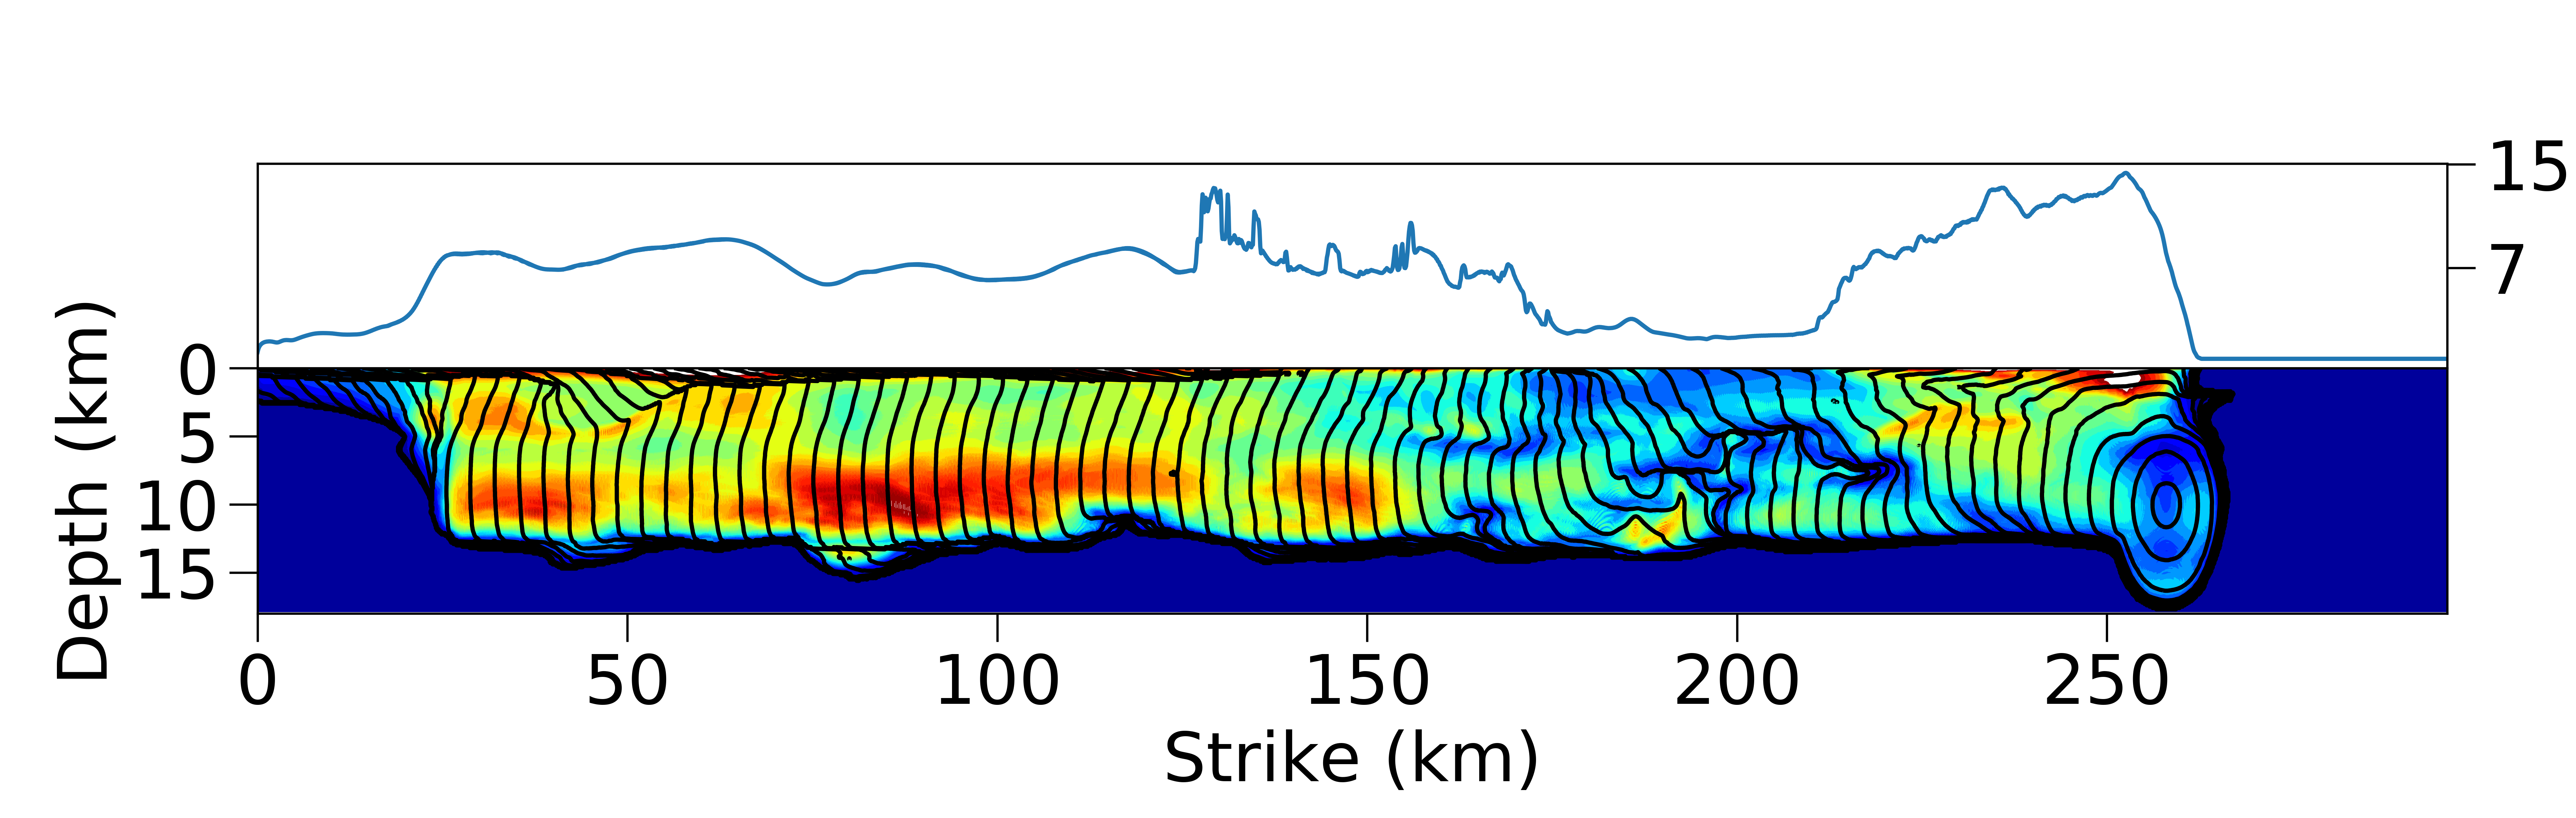
\includegraphics[width=0.9\textwidth]{figures/figure_eks_1a.png}\label{fig:eks-1a}} \\[\baselineskip]%
    \sidesubfloat[]{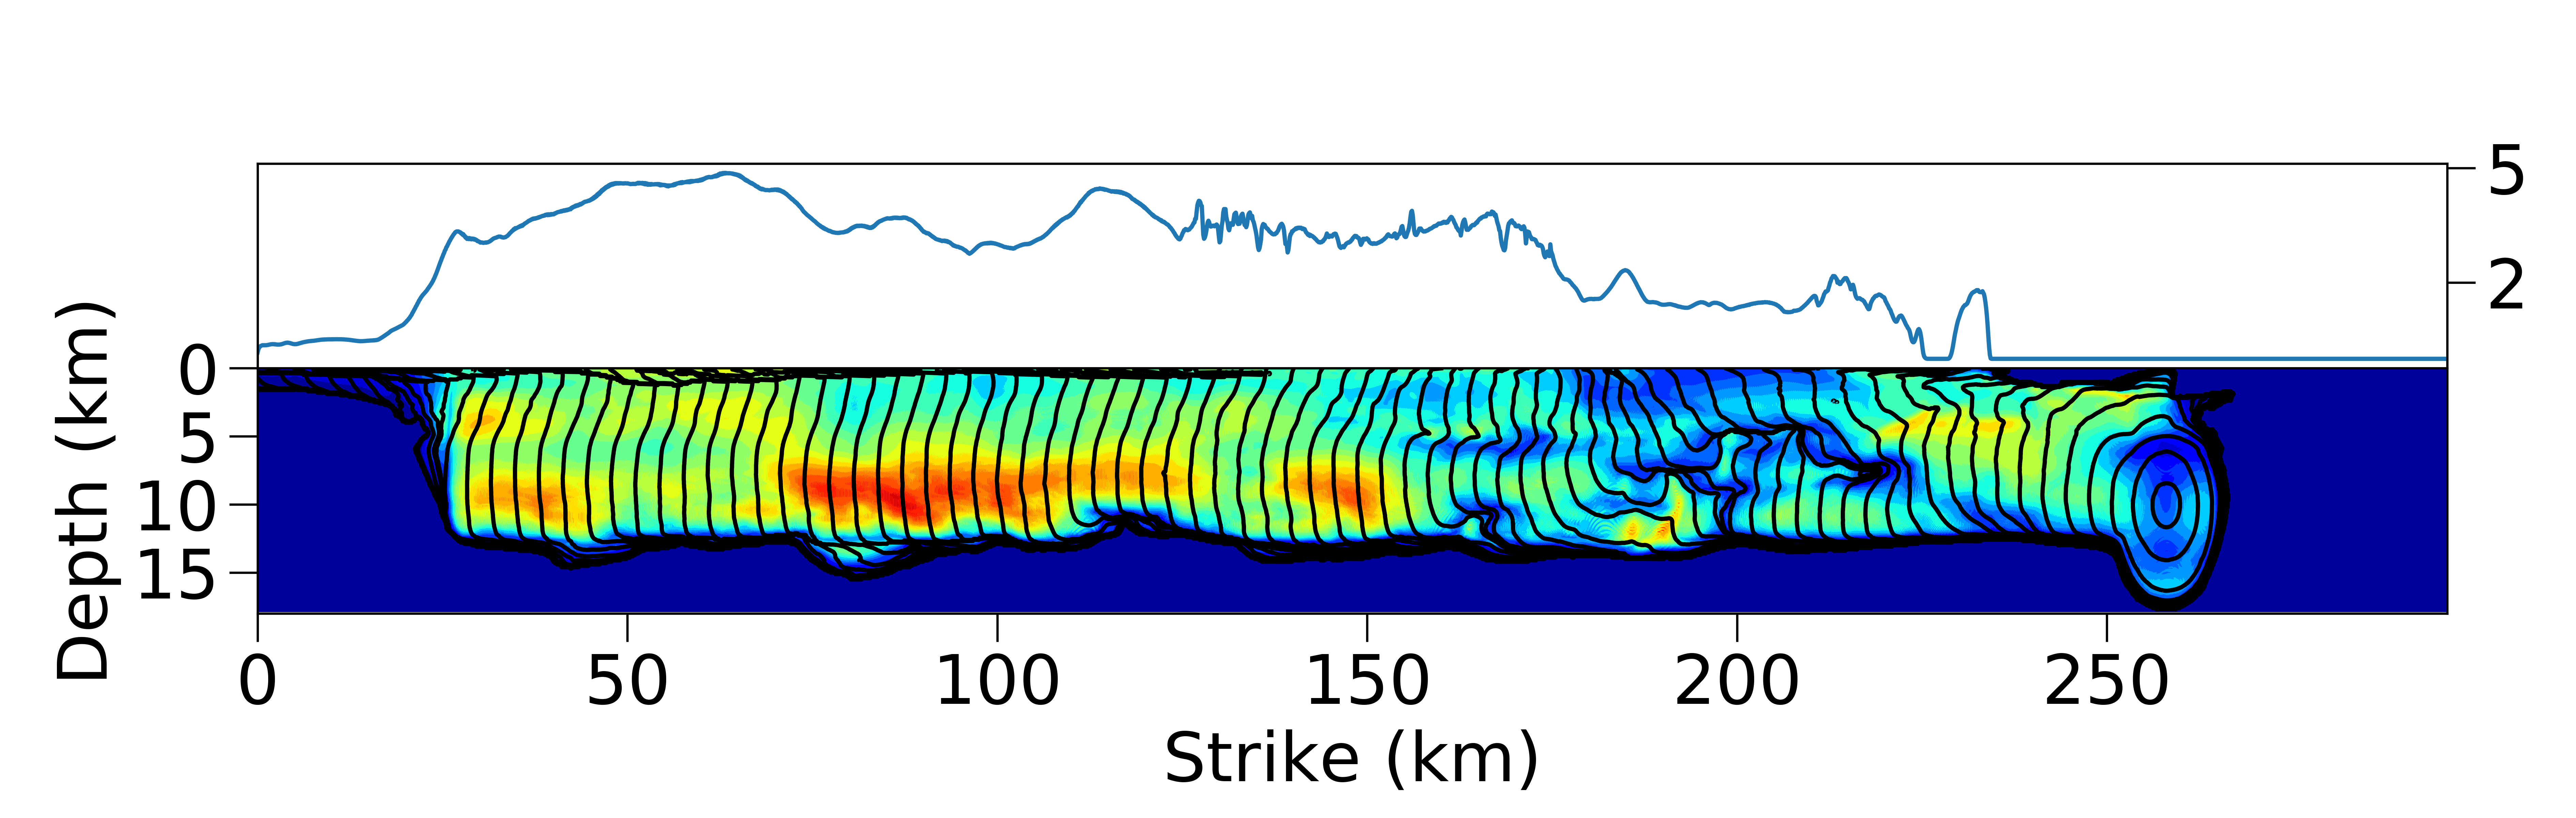
\includegraphics[width=0.9\textwidth]{figures/figure_eks_1b.png}\label{fig:eks-1b}} \\[\baselineskip]%
    \sidesubfloat[]{\includegraphics[width=0.9\textwidth]{figures/figure_eks_1c.png}\label{fig:eks-1c}} \\[\baselineskip]%
    \vspace{-3mm}
    \centering
    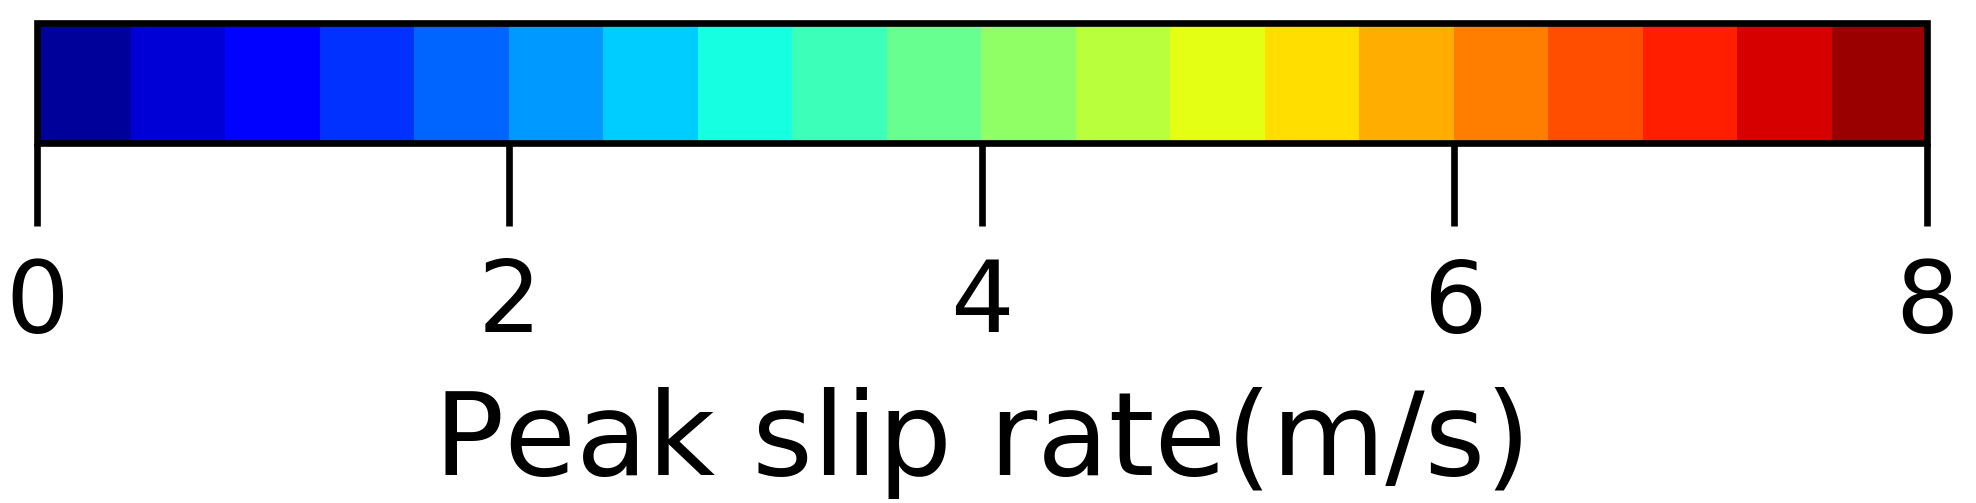
\includegraphics[width=0.3\textwidth]{figures/figure_eks_1d.png}\label{fig:eks-1d}
    \caption{Peak slip rate (PSR) obtained on the fault from a representative rupture case, with the surface PSR (in m/s) shown in the panel above each subplot. From top to bottom shows three models: (a) linear; (b) sandstone (nonlinear); (c) shale (nonlinear). Black contours indicate rupture time in 1 s intervals.}
    \label{fig:eks-1}
\end{figure}
\clearpage

\clearpage
\begin{figure}[!ht]
    \includegraphics[width=0.28\textwidth]{figures/figure_eks_2a.pdf}\label{fig:eks-2a} \hspace{0.02\textwidth}%
    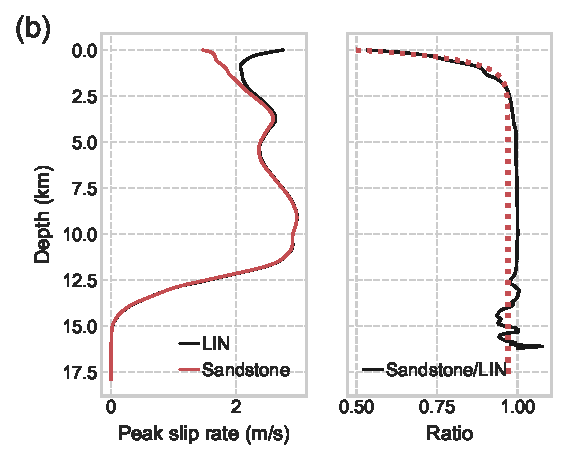
\includegraphics[width=0.28\textwidth]{figures/figure_eks_2b.pdf}\label{fig:eks-2b} \hspace{0.02\textwidth}%\hfil
    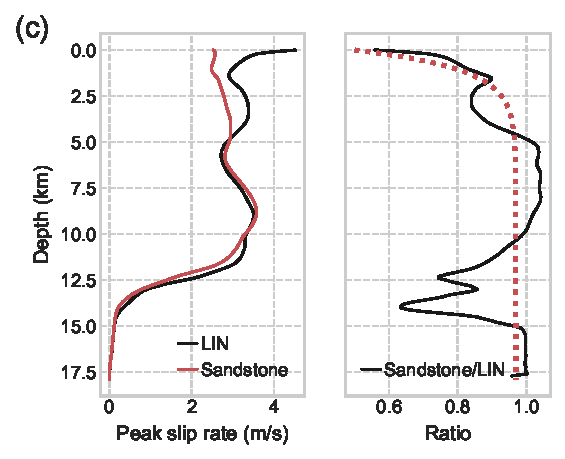
\includegraphics[width=0.28\textwidth]{figures/figure_eks_2c.pdf}\label{fig:eks-2c} % \\[\baselineskip]%
    \caption{Peak slip rate (PSR) averaged over along strike against depth(left panel of each subplot) for sandstone (nonlinear) and linear models and their ratio (right panel of each subplot). (a)-(c) depit three realizations for the sandstone models with stress drop of 7, 8, 10 $MPa$, respectively. Dashed red lines indicates the curves fitting the nonlinear to linear PSR ratio using \cref{eq:eks-2}.}
    \label{fig:eks-2}
\end{figure}
\clearpage


\clearpage
\begin{figure}[!ht]
    \sidesubfloat[]{\includegraphics[width=0.26\textwidth]{figures/figure_eks_3a.pdf}\label{fig:eks-3a}} \hfil
    \sidesubfloat[]{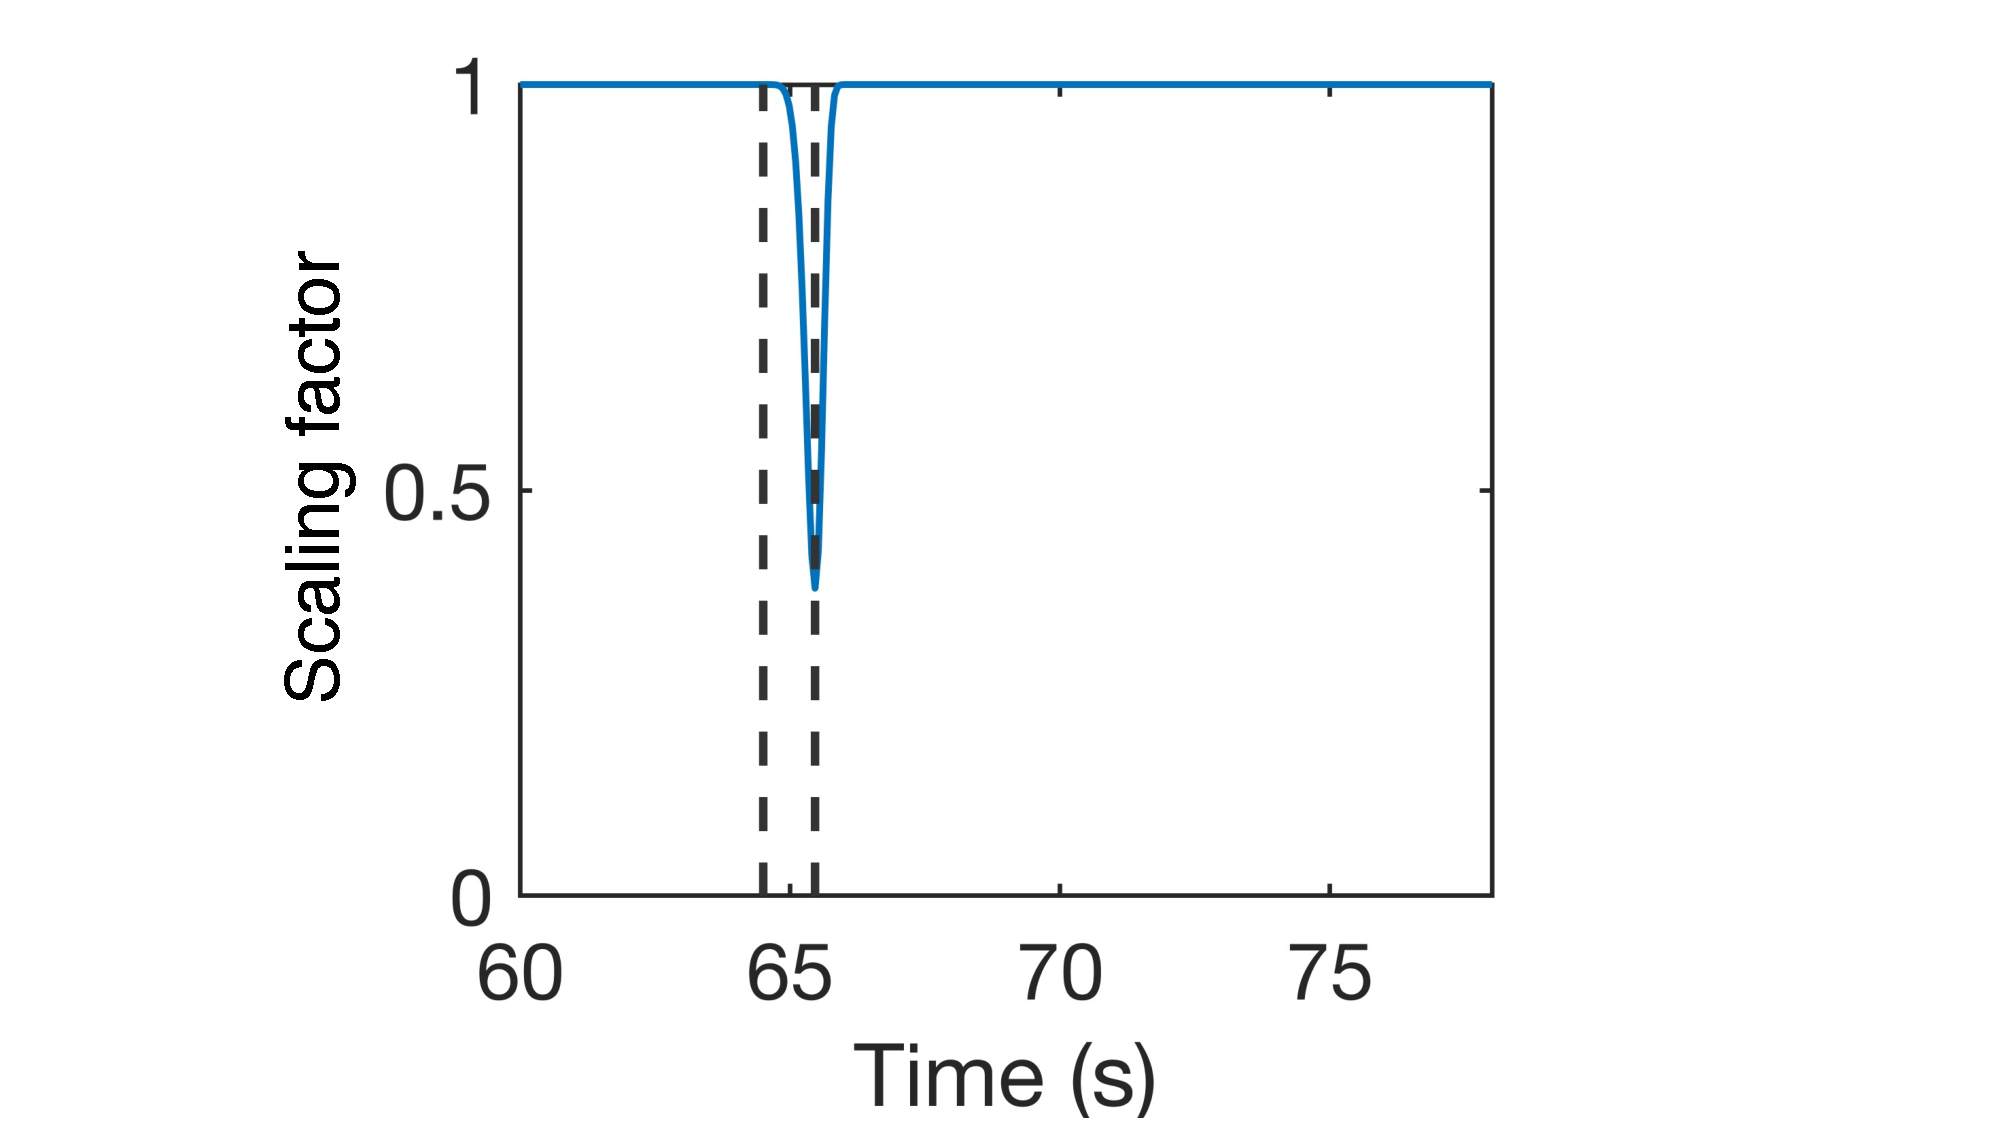
\includegraphics[width=0.26\textwidth]{figures/figure_eks_3b.pdf}\label{fig:eks-3b}} \hfil
    \sidesubfloat[]{\includegraphics[width=0.26\textwidth]{figures/figure_eks_3c.pdf}\label{fig:eks-3c}}
    \caption{(a) The STF on a representative subfault (depth=0) for the linear model. (b) The time-domain scaling factors from the scaling function computed with \cref{eq:eks-2}. For the non-linear model and scaled STF (right). The middle figure shows the conversion function. The black dashed lines in the left and middle figure indicate peak time of the STF and conversion function.}
    \label{fig:eks-3}
\end{figure}
\clearpage

\clearpage
\begin{figure}[!ht]
    \includegraphics[width=0.9\textwidth]{figures/figure_eks_4.png}
    \caption{PGV distribution for the southern San Andreas Fault region, obtained for (a) linear, (b) sandstone and (c) EKS model. Contour lines are just for better visibility. The red dotted rectangle denotes LA basin region for further ground motion comparisons in \Cref{fig:eks-10}.}
    \label{fig:eks-4}
\end{figure}


\clearpage
\floatsetup[figure]{style=plain,subcapbesideposition=top,font=Large,footfont=Large}
\begin{figure}[!ht]
    \sidesubfloat[]{\includegraphics[width=0.4\textwidth]{figures/figure_eks_5a.png}\label{fig:eks-5a}} \hfil%\\[\baselineskip]%
    \sidesubfloat[]{\includegraphics[width=0.4\textwidth]{figures/figure_eks_5b.png}\label{fig:eks-5b}} \\[\baselineskip]%
    \sidesubfloat[]{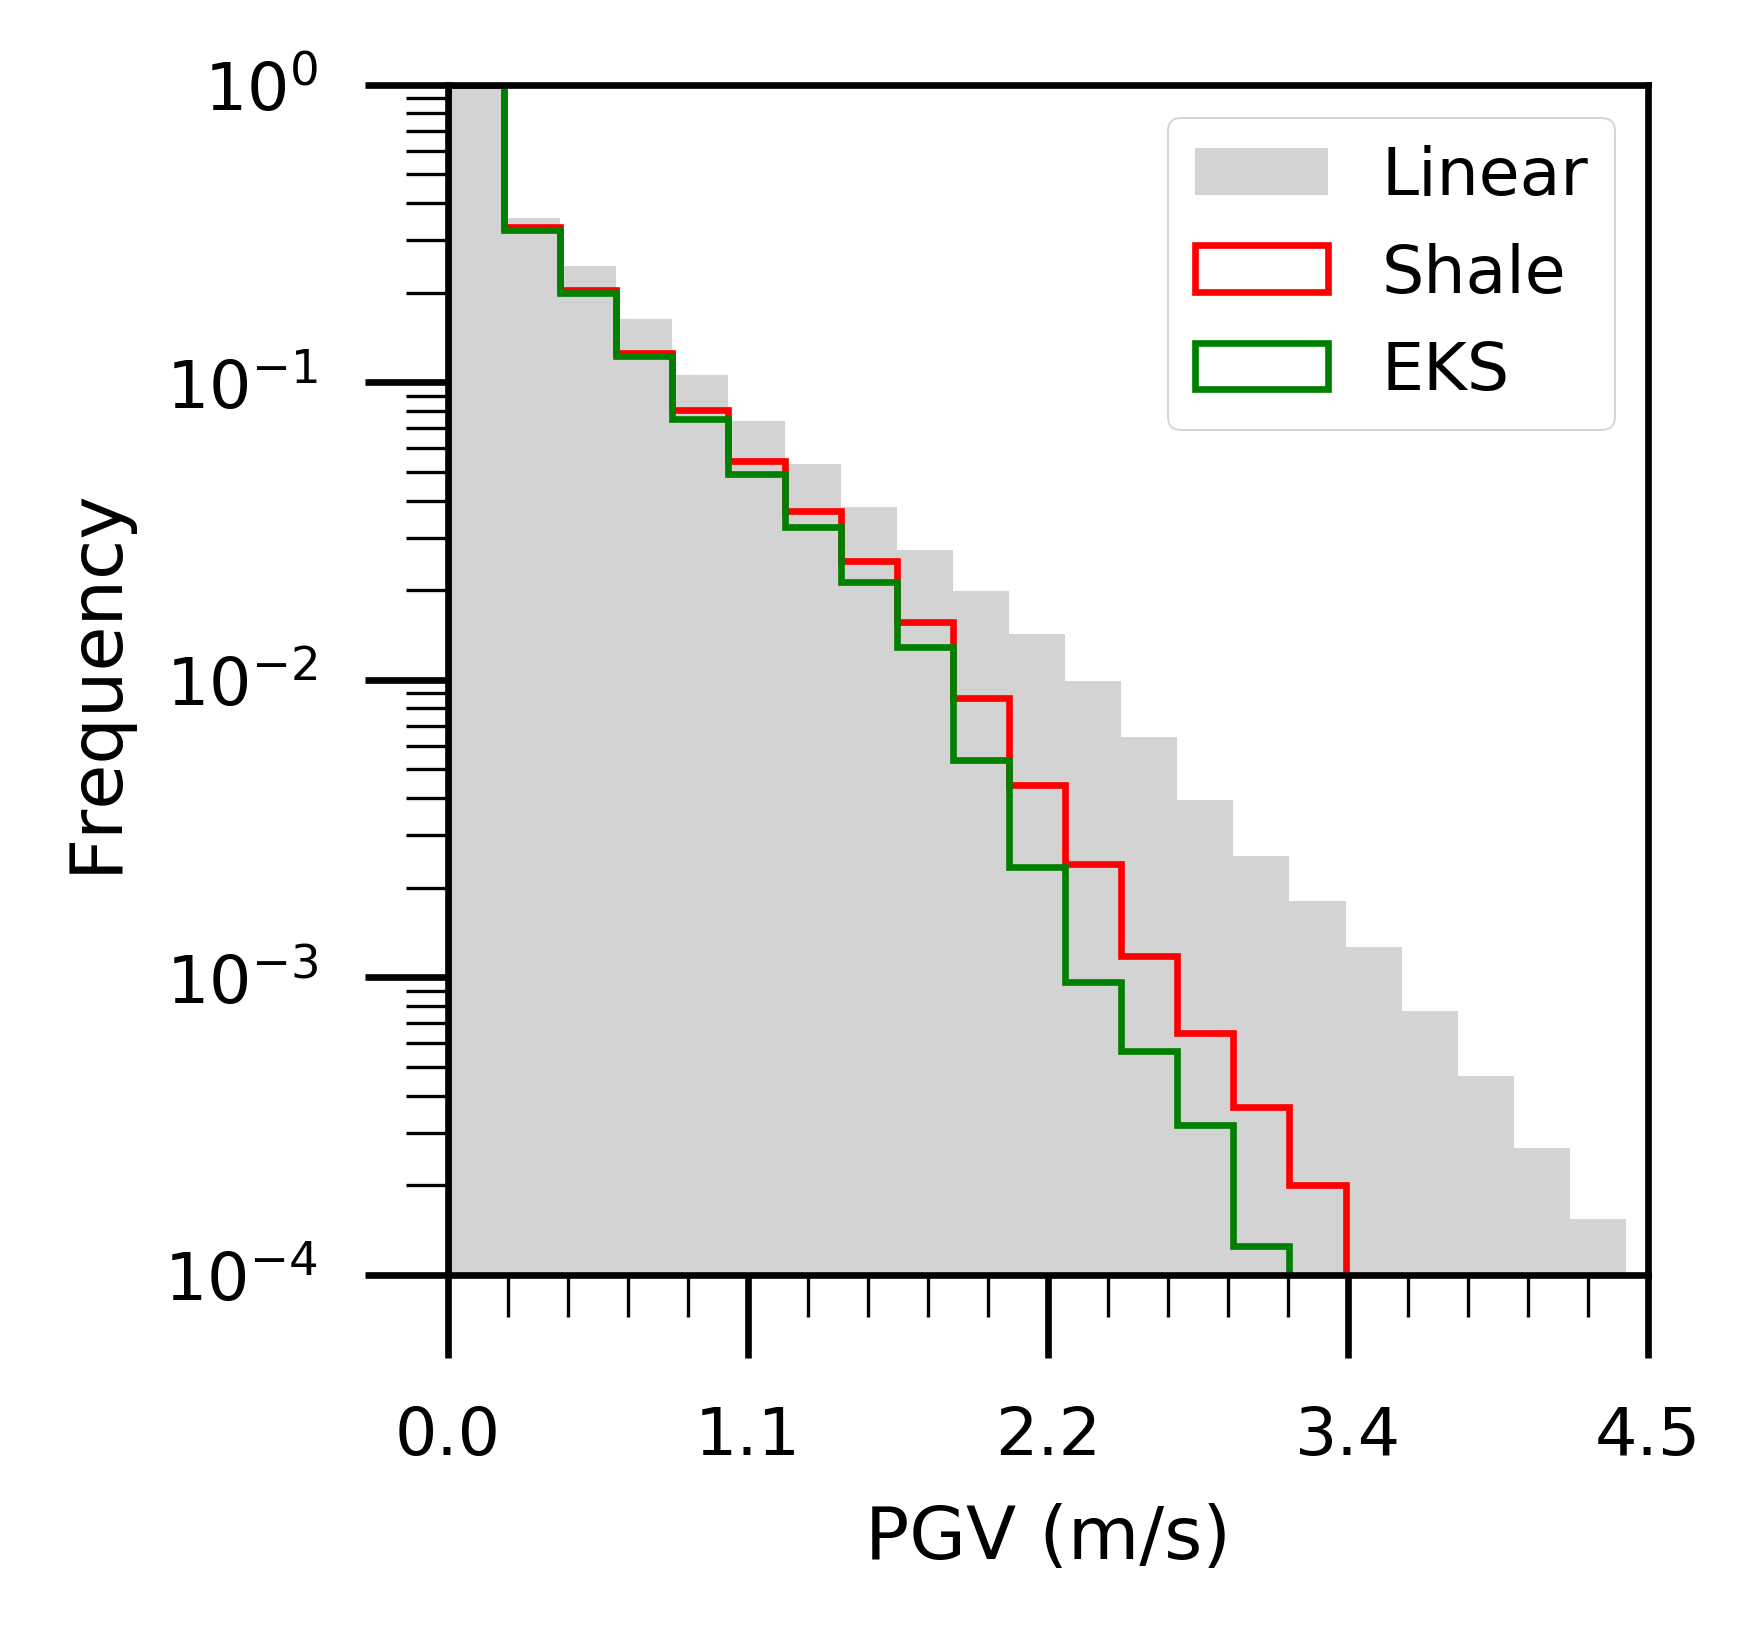
\includegraphics[width=0.4\textwidth]{figures/figure_eks_5c.png}\label{fig:eks-5c}} \hfil%\\[\baselineskip]%
    \sidesubfloat[]{\includegraphics[width=0.4\textwidth]{figures/figure_eks_5d.png}\label{fig:eks-5d}} \\[\baselineskip]

    \caption{Cumulative distribution of PGVs for linear models with stress drop of 7 (a and c) and 10 (b and d) $Mpa$, as well as nonlinear models and the corresponding EKS models. The top row (a and b) depicts nonlinear model with sandstone media and the bottom (c and d) with shale.}
    \label{fig:eks-5}
\end{figure}

\clearpage
\floatsetup[figure]{style=plain,subcapbesideposition=top,font=Large,footfont=Large}
\begin{figure}[!ht]
    \sidesubfloat[]{\includegraphics[width=0.4\textwidth]{figures/figure_eks_6a.pdf}\label{fig:eks-6a}} \hfil%\\[\baselineskip]%
    \sidesubfloat[]{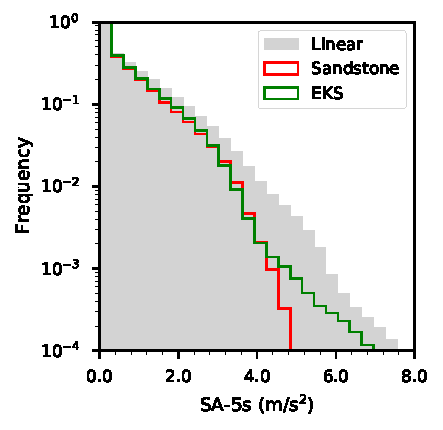
\includegraphics[width=0.4\textwidth]{figures/figure_eks_6b.pdf}\label{fig:eks-6b}} \\[\baselineskip]%
    \sidesubfloat[]{\includegraphics[width=0.4\textwidth]{figures/figure_eks_6c.pdf}\label{fig:eks-6c}} \hfil%\\[\baselineskip]%
    \sidesubfloat[]{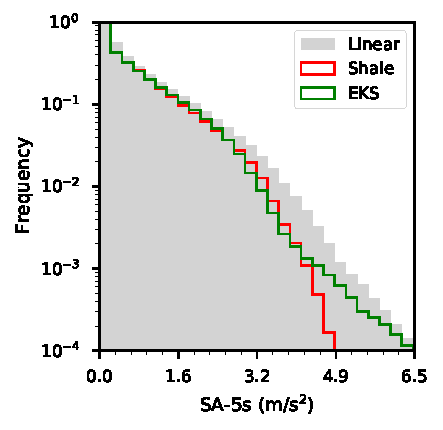
\includegraphics[width=0.4\textwidth]{figures/figure_eks_6d.pdf}\label{fig:eks-6d}}

    \caption{Same as \Cref{fig:eks-5}, but for SA-5s comparisons.}
    \label{fig:eks-6}
\end{figure}

\clearpage
\floatsetup[figure]{style=plain,subcapbesideposition=top,font=Large,footfont=Large}
\begin{figure}[!ht]
    \sidesubfloat[]{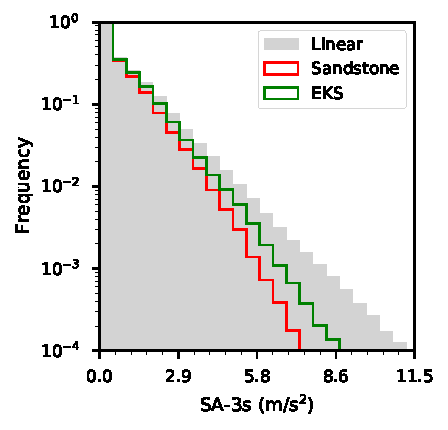
\includegraphics[width=0.4\textwidth]{figures/figure_eks_7a.pdf}\label{fig:eks-7a}} \hfil%\\[\baselineskip]%
    \sidesubfloat[]{\includegraphics[width=0.4\textwidth]{figures/figure_eks_7b.pdf}\label{fig:eks-7b}} \\[\baselineskip]%
    \sidesubfloat[]{\includegraphics[width=0.4\textwidth]{figures/figure_eks_7c.pdf}\label{fig:eks-7c}} \hfil%\\[\baselineskip]%
    \sidesubfloat[]{\includegraphics[width=0.4\textwidth]{figures/figure_eks_7d.pdf}\label{fig:eks-7d}}

    \caption{Same as \Cref{fig:eks-5}, but for SA-3s comparisons.}
    \label{fig:eks-7}
\end{figure}

\clearpage
\floatsetup[figure]{style=plain,subcapbesideposition=top,font=Large,footfont=Large}
\begin{figure}[!ht]
    \sidesubfloat[]{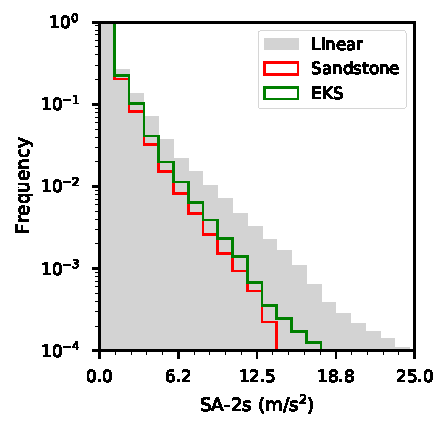
\includegraphics[width=0.4\textwidth]{figures/figure_eks_8a.pdf}\label{fig:eks-8a}} \hfil%\\[\baselineskip]%
    \sidesubfloat[]{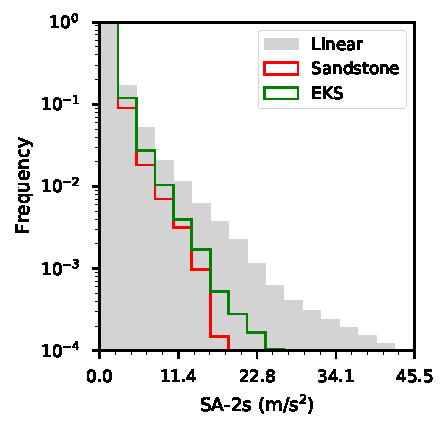
\includegraphics[width=0.4\textwidth]{figures/figure_eks_8b.pdf}\label{fig:eks-8b}} \\[\baselineskip]%
    \sidesubfloat[]{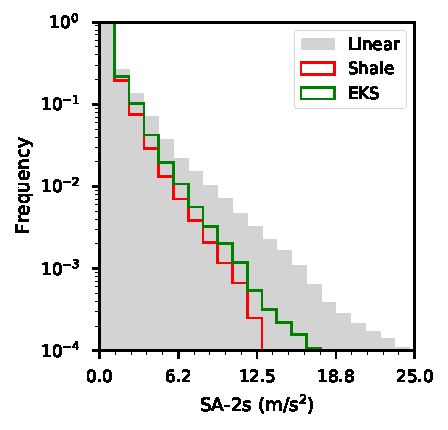
\includegraphics[width=0.4\textwidth]{figures/figure_eks_8c.pdf}\label{fig:eks-8c}} \hfil%\\[\baselineskip]%
    \sidesubfloat[]{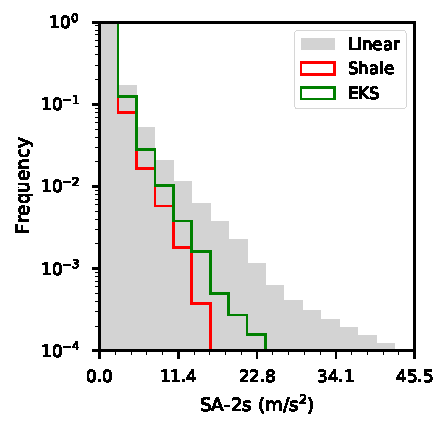
\includegraphics[width=0.4\textwidth]{figures/figure_eks_8d.pdf}\label{fig:eks-8d}}

    \caption{Same as \Cref{fig:eks-5}, but for SA-2s comparisons.}
    \label{fig:eks-8}
\end{figure}

\clearpage
\floatsetup[figure]{style=plain,subcapbesideposition=top,font=Large,footfont=Large}
\begin{figure}[!ht]
    \sidesubfloat[]{\includegraphics[width=0.4\textwidth]{figures/figure_eks_9a.pdf}\label{fig:eks-9a}} \hfil%\\[\baselineskip]%
    \sidesubfloat[]{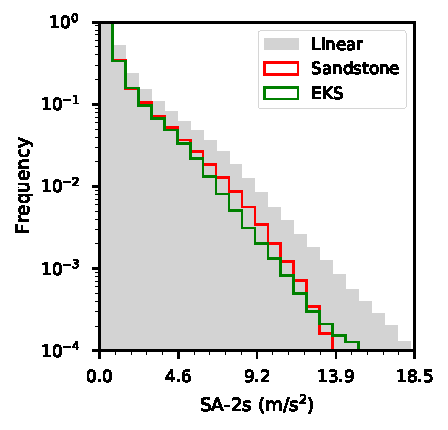
\includegraphics[width=0.4\textwidth]{figures/figure_eks_9b.pdf}\label{fig:eks-9b}} \\[\baselineskip]%
    \sidesubfloat[]{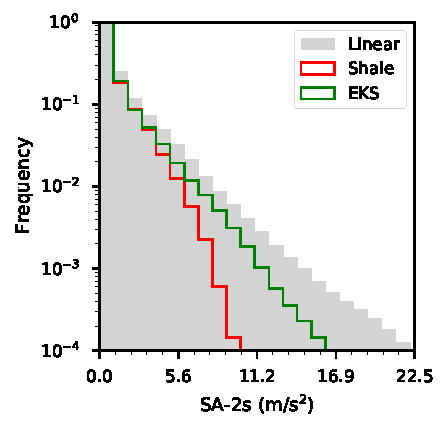
\includegraphics[width=0.4\textwidth]{figures/figure_eks_9c.pdf}\label{fig:eks-9c}} \hfil%\\[\baselineskip]%
    \sidesubfloat[]{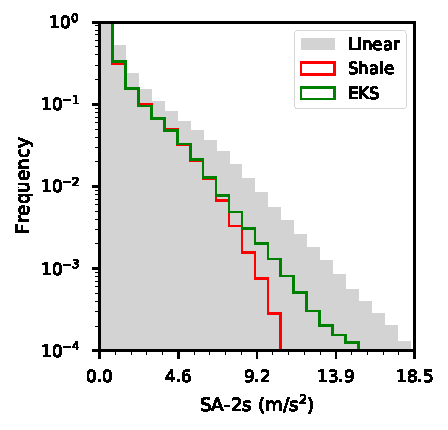
\includegraphics[width=0.4\textwidth]{figures/figure_eks_9d.pdf}\label{fig:eks-9d}}

    \caption{Same as \Cref{fig:eks-8}, but the rupture direction is reversed to NW-SE for all models.}
    \label{fig:eks-9}
\end{figure}


\clearpage
\floatsetup[figure]{style=plain,subcapbesideposition=top,font=Large,footfont=Large}
\begin{figure}[!ht]
    \sidesubfloat[]{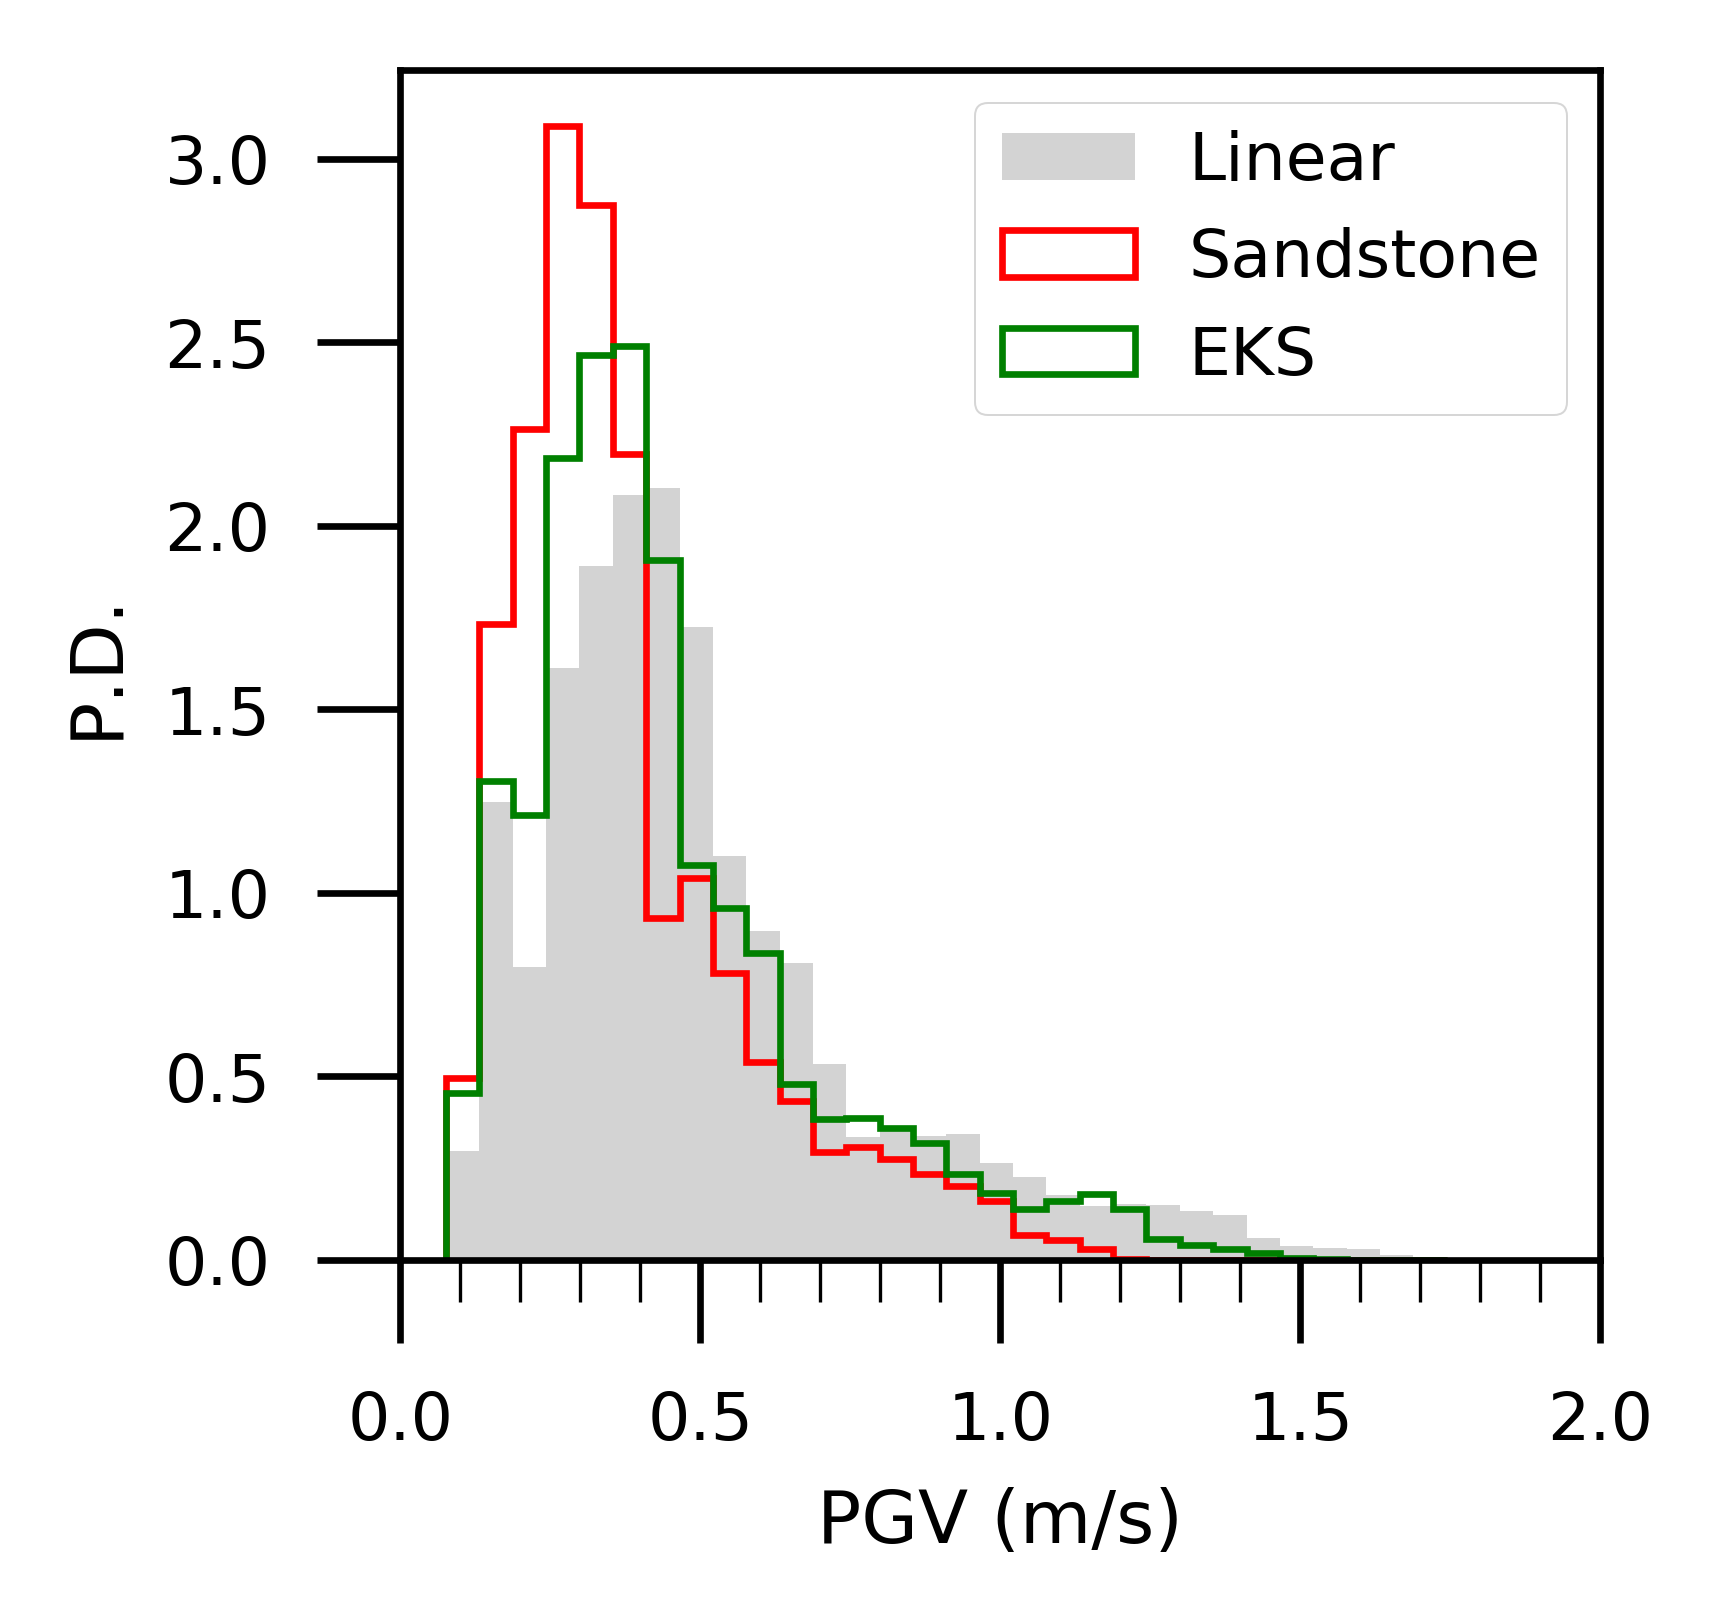
\includegraphics[width=0.4\textwidth]{figures/figure_eks_10a.png}\label{fig:eks-10a}} \hfil%\\[\baselineskip]%
    \sidesubfloat[]{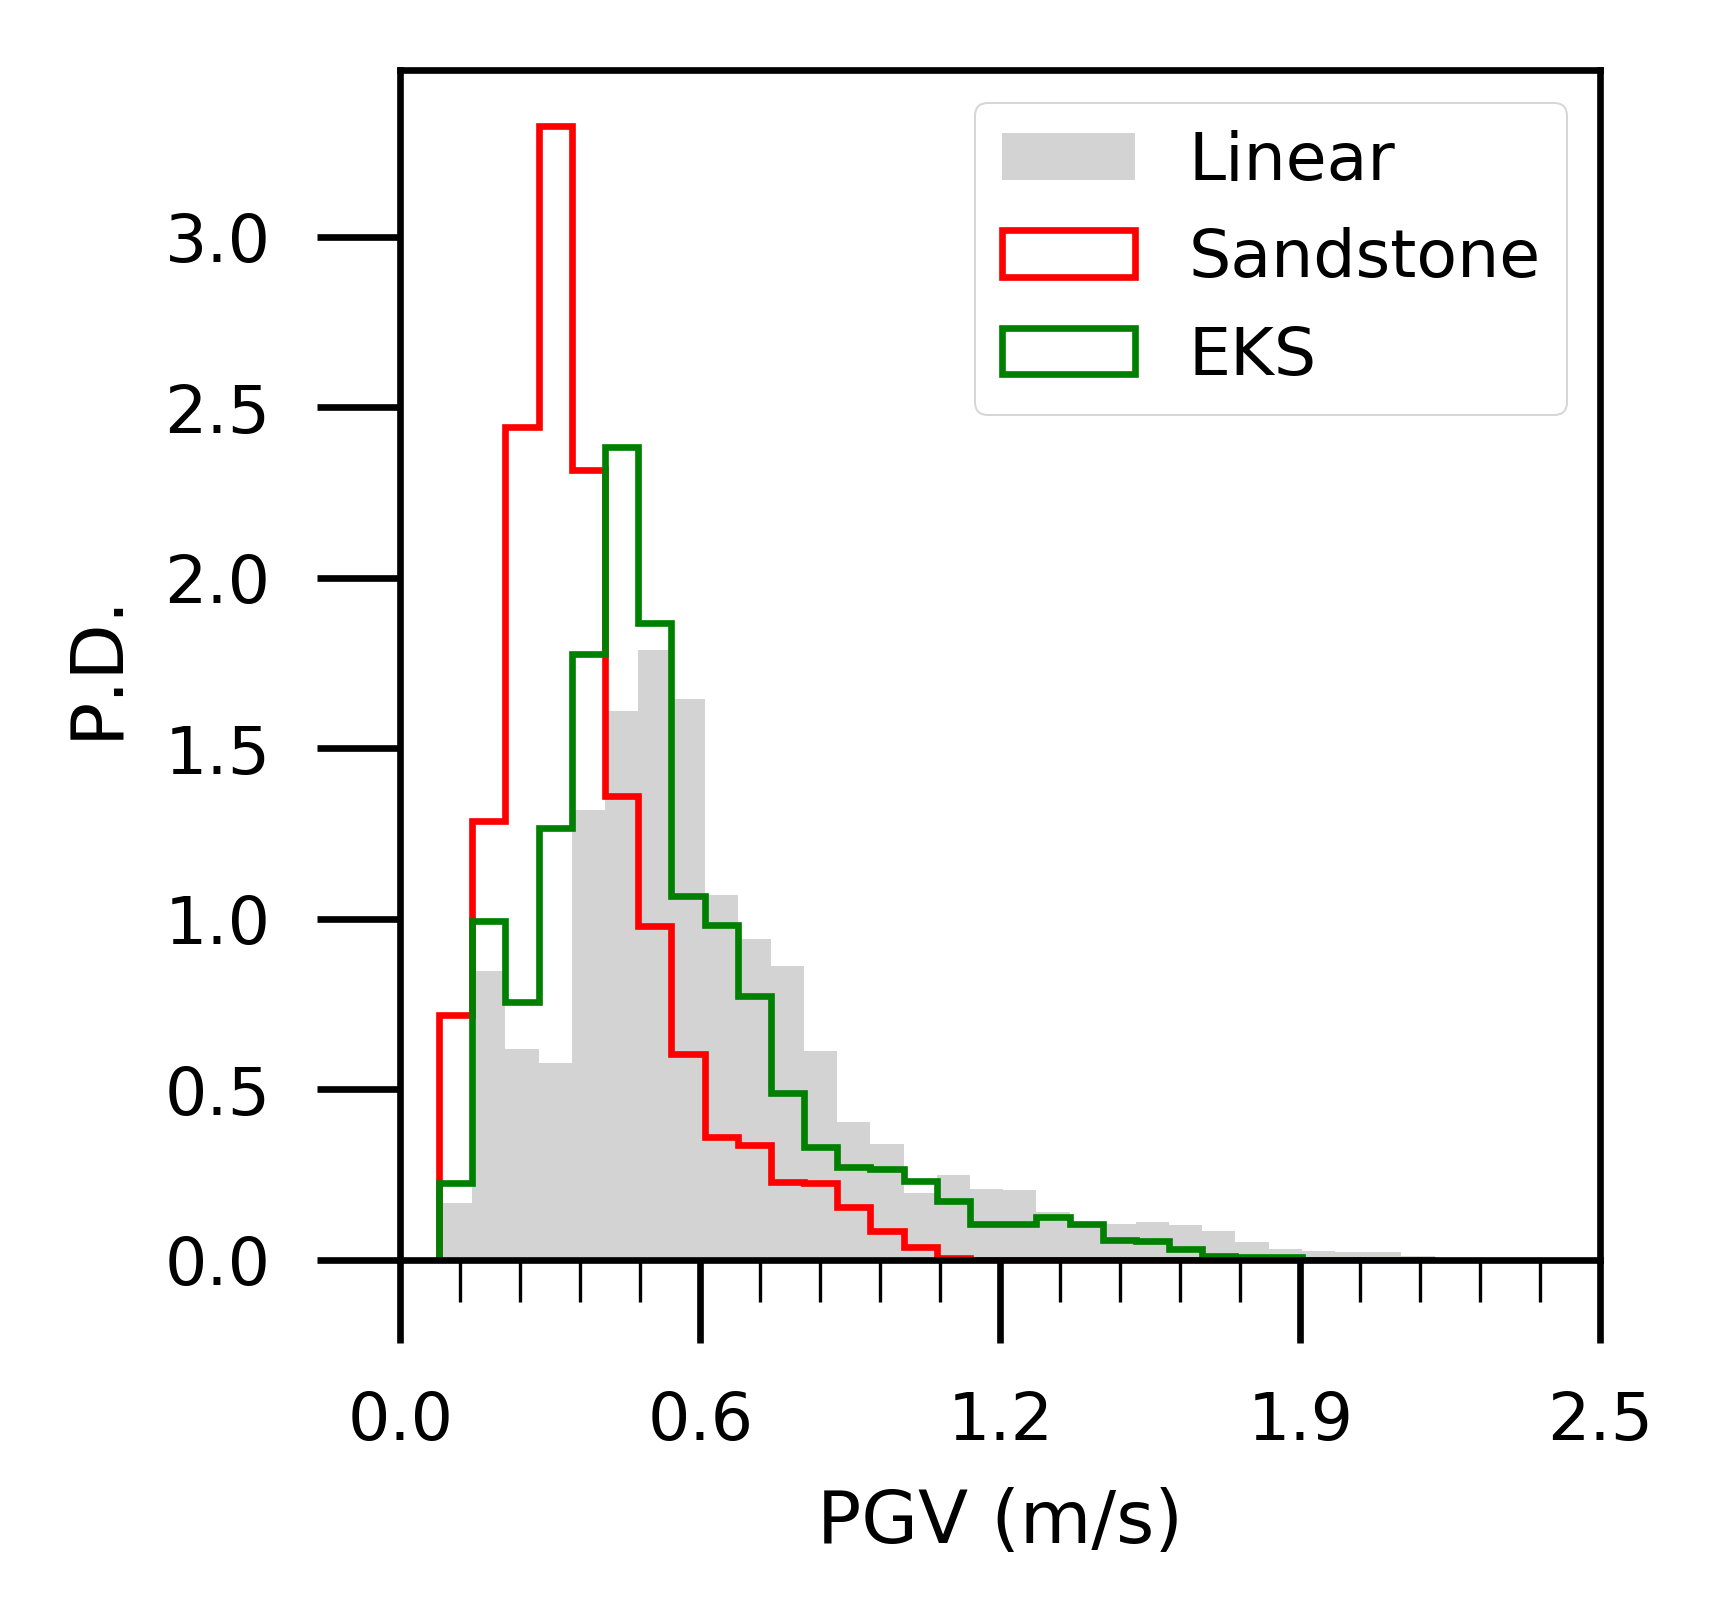
\includegraphics[width=0.4\textwidth]{figures/figure_eks_10b.png}\label{fig:eks-10b}} \\[\baselineskip]%
    \sidesubfloat[]{\includegraphics[width=0.4\textwidth]{figures/figure_eks_10c.png}\label{fig:eks-10c}} \hfil%\\[\baselineskip]%
    \sidesubfloat[]{\includegraphics[width=0.4\textwidth]{figures/figure_eks_10d.png}\label{fig:eks-10d}}

    \caption{Probability densite (P.D) histograms of PGVs in the Los Angeles Basin area. The models shown are the same as in \Cref{fig:eks-5}}
    \label{fig:eks-10}
\end{figure}

\clearpage

%% supplement
% \setcounter{table}{0}
% \setcounter{figure}{0}
% \numberwithin{figure}{chapter}
% \numberwithin{table}{chapter}
% \renewcommand{\thetable}{S\arabic{chapter}.\arabic{table}}
% \renewcommand{\thefigure}{S\arabic{chapter}.\arabic{figure}}
% \newpage
% \section*{Supplementary Materials}
% \addcontentsline{toc}{section}{\protect\numberline{}Supplementary Materials}

% This supplement includes.




\renewcommand{\thetable}{\arabic{table}}
\renewcommand{\thefigure}{\arabic{figure}}

\numberwithin{figure}{chapter}
\numberwithin{table}{chapter}

%\endrefsection
% !TEX encoding = UTF-8 Unicode

\linespread{1.7}
\chapter{Calibration of the Near-surface Seismic Structure in the SCEC Community Velocity Model Version 4}
\linespread{2.0}
%\newrefsection
\label{chap:vs30}

\graphicspath{{/Users/zhh076/work/PhD_way/vs30/}}

The near-surface seismic structure (to a depth of about 1000 m), particularly the shear-wave velocity ($V_S$), can strongly affect the propagation of seismic waves, and therefore must be accurately calibrated for ground motion simulations and seismic hazard assessment. The $V_S$ of the top (< 300 m) crust is often well-characterized from borehole studies, geotechnical measurements, and water and oil wells, while the velocities of the material deeper than about 1000 m are typically determined by tomography studies. However, in regions lacking information on shallow lithological stratification, typically rock sites outside the sedimentary basins, the material parameters between these two regions are typically poorly characterized due to resolution limits of seismic tomography. When the alluded geological constraints are not available, models, such as the Southern California Earthquake Center Community Velocity Models (CVMs), default to regional tomographic estimates that do not resolve the uppermost $V_S$ values, and therefore deliver unrealistically high shallow $V_S$ estimates. A widely-used method for incorporating the near-surface earth structure is implemented in CVMs by applying a generic overlay based on measurements of time-averaged $V_S$ in top 30 m ($V_{S30}$) to taper the upper part of the model to merge with tomography at certain depth (e.g., 350 m). However, our 3D simulations of the 2014 $M_w$ 5.1 La Habra earthquake in the Los Angeles area using the CVM-S4.26.M01 model significantly underpredict low-frequency (< 1 Hz) ground motions at sites subject to the generic overlay (``taper''). On the other hand, extending the $V_{S30}$-based taper of the shallow velocities down to a depth of about 1000 meters improves the fit between our synthetics and seismic data at those sites, without compromising the fit at well constrained sites. We explore various tapering depths, demonstrating increasing amplification as the tapering depth increases, and the model with 1000 m tapering depth yields overall favorable results. Effects of varying anelastic attenuation are small compared to effects of velocity tapering. Although a uniform tapering depth is adopted in the models, we observe some spatial variabilities that may further improve our method.


%%%%%%%%%%%%%%%%%%%%%%%%%%
\section{Introduction} \label{vs30:intro}
Ground motion amplification due to the near-surface structure is widely accepted and well-studied \citeg{gilbertSanFranciscoEarthquake1907,fieldModifiedGroundMotionAttenuation2000}, and needs to be incorporated in numerical  simulations of earthquakes to produce accurate ground motion results. Theoretical analyses have shown that the near-surface shear-wave velocity ($V_S$) can exert strong control on spectral amplification \citep{joynerEffectQuaternaryAlluvium1981,booreEstimationGroundMotion1991,andersonControlStrongMotion1996,dayRMSResponseOnedimensional1996}. The time-averaged shear-wave velocity in the upper 30 m ($V_{S30}$) is routinely used as a representation of the site condition in ground motion prediction models and building codes \citep{borcherdtEstimatesSiteDependentResponse1994,bozorgniaNGAWest2ResearchProject2014,internationalcodecouncil2015IBCInternational2014}. Several methods have been proposed for estimating $V_{S30}$ from topography \citep{waldTopographicSlopeProxy2007}, supplemented with near-surface geological information \citep{thompsonVS30MapCalifornia2014,willsNextGeneration302015}. However, despite the continuing advancement in the $V_{S30}$-based methodologies by the seismic hazard community \citeg{thompsonVS30MapCalifornia2014,heathGlobalHybrid302020},  estimating $V_{S30}$ at high resolution remains a difficult task and it is noted that $V_{S30}$ is not a good single proxy for the estimation of site amplification \citeg{steidlSiteResponseSouthern2000,leeShouldAverageShearwave2010,shingakiEvaluationPerformanceSite2018}. Other empirical methodologies provide additional predictive capability for shallow low-velocity amplification, normally constrained by sediment depth, which is parameterized using the depth to the 1 km/s ($z_1$) or 2.5 km/s ($z_{2.5}$) $V_S$ horizon \citeg{abrahamsonSummaryASK14Ground2014,booreNGAWest2EquationsPredicting2014,campbellNGAWest2GroundMotion2014}. Nonetheless, these empirical methods, oftentimes dependent on $V_{S30}$, have similar limitations with $V_{S30}$ that depth-dependent and lateral velocity variations are insufficiently accounted for.

While the current approximations to correct for site effects represent great progress in ground motion estimation, a fully physics-based approach to computing ground motion offers opportunities for further improvements. The physics-based approach entails difficult challenges as well, and remains a long-term goal. In such an approach, the full wavefield is computed deterministically, to maximum frequencies that are sometimes up to 5 Hz or higher, using a 3D velocity model that includes observationally constrained heterogeneities \citep{savranGroundMotionSimulation2019,withersGroundMotionIntraevent2019,hu05HzDeterministic2021}. A necessary ingredient in producing accurate synthetic seismograms using physics-based simulations is an accurate velocity model for the model region. Community Velocity Models (CVMs) have been developed for such purpose, e.g., the Southern California Earthquake Center (SCEC) CVMs \citep{smallSCECUnifiedCommunity2017}, the Cascadia CVM \citep{stephensonCascadiaSubductionZone2017} and the Subsurface Structure Model maintained by the Japan Seismic Hazard Information Station \citep{fujiwaraJSHISINTEGRATEDSYSTEM2017}. These velocity models are often generated by combining 3D tomographic inversion from seismic waves \citep{tapeAdjointTomographySouthern2009,tapeSeismicTomographySouthern2010,leeFull3DTomographyCrustal2014} with shallow geotechnical information (e.g., $V_{S30}$). The spatial resolution of large-scale tomographic studies is generally limited by the density of ray paths, distribution of high-quality measurements, or intrinsic nonuniqueness of inversion, particularly in the upper ~1000 m of the crust. For example, \citet{linThreedimensionalCrustalSeismic2007} had a vertical grid spacing of 3 km and only resolved > 1 km velocity contrasts in their tomographic inversion using P and S wave arrival time, the full-3D seismic waveform tomography conducted by \citet{leeFull3DTomographyCrustal2014} can reach at best 1 km resolution in the center of the inverted region, and \citet{qiuEikonalTomographySouthern2019} found the top 3 km is poorly constrained in their Eikonal tomography using ambient noise cross correlations.

While the current approximations to correct for site effects represent great progress in ground motion estimation, a fully physics-based approach to computing ground motion offers opportunities for further improvements. The physics-based approach entails difficult challenges as well, and remains a long-term goal. In such an approach, the full wavefield is computed deterministically, to maximum frequencies that are sometimes up to 5 Hz or higher, using a 3D velocity model that includes observationally constrained heterogeneities \citep{savranGroundMotionSimulation2019,withersGroundMotionIntraevent2019,hu05HzDeterministic2021}. A necessary ingredient in producing accurate synthetic seismograms using physics-based simulations is an accurate velocity model for the model region. Community Velocity Models (CVMs) have been developed for such purpose, e.g., the Southern California Earthquake Center (SCEC) CVMs \citep{smallSCECUnifiedCommunity2017}, the Cascadia CVM \citep{stephensonCascadiaSubductionZone2017} and the Subsurface Structure Model maintained by the Japan Seismic Hazard Information Station \citep{fujiwaraJSHISINTEGRATEDSYSTEM2017}. These velocity models are often generated by combining 3D tomographic inversion from seismic waves \citep{tapeAdjointTomographySouthern2009,tapeSeismicTomographySouthern2010,leeFull3DTomographyCrustal2014} with shallow geotechnical information (e.g., $V_{S30}$). The spatial resolution of large-scale tomographic studies is generally limited by the density of ray paths, distribution of high-quality measurements, or intrinsic nonuniqueness of inversion, particularly in the upper ~1000 m of the crust. For example, \citet{linThreedimensionalCrustalSeismic2007} had a vertical grid spacing of 3 km and only resolved > 1 km velocity contrasts in their tomographic inversion using P and S wave arrival time, the full-3D seismic waveform tomography conducted by \citet{leeFull3DTomographyCrustal2014} can reach at best 1 km resolution in the center of the inverted region, and \citet{qiuEikonalTomographySouthern2019} found the top 3 km is poorly constrained in their Eikonal tomography using ambient noise cross correlations.


Shallow velocity structure, e.g. S-wave impedance and scattering, has an significant role in modifying ground motion amplification and duration \citeg{graves1995preliminary,andersonControlStrongMotion1996,imperatoriBroadbandNearfieldGround2013}. Specifically, 1D theoretical analysis by \citet{dayRMSResponseOnedimensional1996} suggests that the smoothed amplification spectrum is principally determined by shallow $V_S$, above roughly the depth of half the smoothing bandwidth expressed as a wavelength. Over a ~0.5 Hz bandwidth and typical Southern California rock site $V_S$ values, the analysis predicts that the $V_S$ structure above about 1000 m will have a disproportionately strong effect on ground motion. Therefore, resolving the shallow velocity structure is essential in accurate predictions of ground motions. In SCEC CVMs, velocities and densities in the top 300 m within the basins are constrained by geotechnical and geophysical data, such as seismic reflection surveys, borehole seismic records and gravity data, and in the deeper basins are estimated either from empirical age- and depth-consolidation rules based on water and oil wells and geological studies, or sonic logs and reflection/refraction profiles from the oil industry \citep{magistraleGeologybased3DVelocity1996,magistraleSCECSouthernCalifornia2000,sussWaveSeismicVelocity2003}. Unfortunately, outside and below the basins (typically rock sites), CVMs simply assign interpolated results from regional tomography studies. Additional data constraints on shallow velocity structure, including seismic refraction studies \citeg{teagueMeasuredVsPredicted2018} or borehole logs \citeg{stellerNewBoreholeGeophysical1996,thompsonTaxonomySiteResponse2012} are rare in these regions.

Where location-specific constraints are lacking, previous studies have attempted to use generic models to bridge the gap between data constraints at shallow (<~30 m) and deeper (>~1000 m) depths. For example, \citet{booreSiteAmplificationsGeneric1997} generated a continuous depth-dependent $V_S$ function based on 3 different intervals. The $V_S$ profile in the upper 30 m was constructed from interpolated shallow average arrival times. At depths below 4 km, $V_S$ was estimated from the P-wave velocity ($V_P$), measured from earthquake location studies and velocity surveys, on the assumption of a fixed Poisson ratio at 0.25. Finally, the shallow and deeper $V_S$ were connected using two power-law functions. \citet{elyVs30derivedNearsurfaceSeismic2010} proposed a generalized method that derives the surface $V_S$ by linearly scaling $V_{S30}$ and then interpolates velocities with depths until converging to the original tomography model at a certain depth, a scheme which has been implemented in some of the SCEC CVMs. We will use the term ``tapering'' to denote the replacement of (poorly constrained) site-specific CVM values by a generic function of depth that merges smoothly with the original CVM at some depth $z_T$. \citet{elyVs30derivedNearsurfaceSeismic2010} proposed a value of 350 m for $z_T$, based on qualitative comparison between synthetic and seismic records from the 2008 $M_w$ 5.4 Chino Hills, CA, earthquake.

In this study, we quantify the accuracy of ground motion simulations based upon comparisons to the 2014 $M_w$ 5.1 La Habra, CA, earthquake, and interpret the results in terms of the representation of crustal $V_S$ in the top 1000 m. The paper is organized as follows: we first briefly introduce our numerical approach to obtain the simulated ground motions, present an approximate 1D analysis of site amplification to evaluate the potential to improve site amplification at poorly constrained sites, and finally evaluate different generic tapers using 3D wave propagation simulations. The proposed tapering method amplifies the ground motions as the tapering depths increase, which generates up to 3 times (less than 10\%) increase in the spectral amplitudes at poorly (well) constrained locations, compared to the original (i.e., untapered) CVM. We also discuss the limitations of this study, in particular the neglect of spatial variation of the taper depths, which will be a future objective to investigate, using more validation metrics and higher frequencies.



% %%%%%%%%%%%%%%%%%%%%%%%%%%%%%%%
\section{Numerical Approach}\label{vs30:approach}
We perform 0-1 Hz wave propagation simulations of the 2014 $M_w$ 5.1 La Habra earthquake to explore the accuracy of ground motion predictions in terms of the shallow velocity structure. The simulations use the SCEC velocity model CVM-S4.26-M01 (hereafter referred to as CVM-S). Fig. 1 shows the computational domain and strong motion seismic stations in the greater Los Angeles area used in this study. We discretize a 148 km $\times$ 140 km $\times$ 58 km region from CVM-S and the computational domain is rotated 39.9$^\circ$ clockwise to reduce the mesh size while optimizing the data coverage in our region of interest. \Cref{tab:vs30-1} lists the simulation parameters.

The GPU-supported staggered-grid finite difference code AWP-ODC \citep[Anelastic Wave Propagation - Olsen, Day, and Cui, from the authors of the code;][]{cuiScalableEarthquakeSimulation2010} with discontinuous mesh \citep{nieFourthOrderStaggered2017} was used for the simulations analyzed in this study. We used spatial grid spacings of 20 m and 60 m in the grid partitions above and below 7.5 km, respectively, and a minimum $V_S$ of 500 m/s. To facilitate the use of these simulations in a companion, high-frequency study \citep{hu05HzDeterministic2021}, we computed frequencies up to 5 Hz. However, we restrict our analysis to a maximum frequency of 1 Hz in this study, which precludes some of the complicating effects that may become important at higher frequencies, e.g. topography, frequency-dependent attenuation, etc.  We also verified that reducing the minimum $V_S$ to 200m/s makes only negligible difference to the spectral amplifications of interest (see \cref{fig:vs30-S1}). Anelastic attenuation is incorporated with the quality factors given by linear velocity-dependent relations $Q_S=0.1V_S$ ($V_S$ in m/s) and $Q_P=2Q_S$, as suggested by previous results \citep{bielakShakeOutEarthquakeScenario2010,withersGroundMotionIntraevent2019}. We applied sponge zones \citep{cerjanNonreflectingBoundaryCondition1985} with a width of 64 nodes at the exterior grid boundaries (except at the flat free surface) to limit artificial reflections.

The 2014 $M_w$ 5.1 La Habra earthquake was well recorded by broadband strong motion sensors. We selected 259 stations with the epicentral distance up to 90 km and signal-to-noise larger than 3 dB for our study. The assessment of the ground motion synthetics is made using the Fourier amplitude spectra (FAS) of accelerations at all 259 stations, and the goodness of fit to data is described by the FAS bias between model and data:

\begin{equation}\label{eq:vs30-1}
  Bias(frequency, site)=\log_{10}\left(\frac{F A S_{\text {model }}}{F A S_{\text{data }}}\right)
\end{equation}

We used a kinematic source description generated following \citet{gravesKinematicGroundMotion2016} which creates finite-fault rupture scenarios with stochastic characteristics optimized for California events. The focal mechanism was taken from the U.S. Geological Survey \citep[strike=233$^\circ$, dip=77$^\circ$, rake=49$^\circ$;][]{usgsEarthquakeEventsFocal2014} with a moment magnitude 5.1, fault area of 2.5 km $\times$ 2.5 km, and a hypocentral depth of 5 km (0.5 km below the top of the finite fault). The source was selected from a series of 40 realizations with different random seeds from comparison between spectral accelerations with records at stations within 31 km to the epicenter (R. Graves, Personal Communication, 03/04/2020; see \Cref{fig:vs30-2}). The rupture duration is less than 2 s, and the source model was sampled at an interval of 0.001 s, identical to the time step used in our simulations.

The $V_S$ profiles extracted from CVM-S beneath all 259 stations selected for the La Habra event are shown in \Cref{fig:vs30-3}. For most stations, the unmodified CVM-S gives low surface $V_S$ (< 500 m/s, see \cref{fig:vs30-3}a), while a small portion (15\%) of the stations have significantly larger surface $V_S$ (> 1500 m/s, up to 4650 m/s). Such large $V_S$, typically representative of much larger depths, are highly unrealistic at the surface in western North America, even for rock sites in the presence of weathering (note that shallow velocities can be much higher in mid-continent and eastern North America where the surface weathered soils are stripped off by glacial erosion). Additionally, the fact that the $V_S$ values remain constant between the surface and about 500 m depth (\cref{fig:vs30-3}) indicates a poorly constrained near-surface $V_S$ at these stations. We separate all sites into two classes: type A sites where CVM-S provides meaningful near-surface velocities based on geological and geophysical constraints and type B sites where shallow velocities are typically higher than realistic near-surface velocities due to their derivation from relatively low-resolution seismic tomography. The two types of stations fall into two distinct CVM-S surface $V_S$ classes, ~200-300 m/s and ~1500-4650 m/s, respectively (\cref{fig:vs30-3}). Type B represents sites with poor constraints in velocities and thus constitute our main target for calibration in this study (see \cref{tab:vs30-2} for type B site information from the original, untapered CVM-S; note the unrealistically large surface $V_S$). There are many indications that the near-surface $V_S$ values at type B sites in CVM-S are anomalously high. CVM-S includes a geotechnical layer (GTL) by recovering the basin information from geological and geophysical data, which are typically confined to the top 300 m in basin areas only \citep{magistraleGeologybased3DVelocity1996,magistraleSCECSouthernCalifornia2000}. In addition, CVM-S cuts off the GTL at 350 m depth when it is merged with the background velocity model, leading to a sharp contrast at that depth when the background model has high velocity (as at type B sites). Note, that the mean values of each of the two groups of profiles become similar below a depth of 2000 m. The hypocentral-distance distributions for the respective site types (A and B) are similar, though type B sites are typically located outside the basins and thus of relatively larger distance.

\section{Simulation Results}
We calculate the Fourier amplitude spectra (FAS) of accelerations for both recorded and synthetic time series, both processed in the following way: (1) low-pass filtering with a corner frequency of 10 Hz using a 4$^{\text{th}}$-order zero-phase Butterworth filter; (2) interpolating linearly to a uniform time step; (3) tapering at the last 2 seconds using the positive half of a Hanning window; and (4) padding with 5 seconds of zeros. Horizontal components for both data and synthetics were rotated to east-west (E-W) and north-south (N-S) directions, and the data were synchronized to the rupture time. Furthermore, if needed, records were padded with zeros to obtain a duration of 120 s relative to the rupture time. Finally, we calculated the FAS of the accelerations from the time derivatives of the velocities for the synthetics and records, which were bandpass filtered between 0.15 Hz and 1 Hz using a 4$^{\text{th}}$-order zero-phase Butterworth filter. The lower cut-off frequency of 0.15 Hz was selected to avoid noise interference.

\Cref{fig:vs30-4} shows a comparison of median FAS, taken over the two types of stations, of ground accelerations for synthetics from unmodified CVM-S and recordings. The FAS at type A sites are well predicted, especially below 0.7 Hz, with a small underprediction between 0.7 Hz and 1 Hz on the horizontal components. At type B sites, however, significant underprediction is observed for all three components for frequencies as low as 0.2 Hz on the horizontal components. Also, as the frequency increases toward 1 Hz, the difference in FAS between data and synthetics increases rapidly, leaving the FAS from the simulated results outside of the 95\% confidence interval of the data. The relatively good match at type A sites indicates that the source description is not likely to be a significant source of the misfit. Furthermore, more complicated path and site effects from topography, small-scale heterogeneities and frequency-dependent attenuation are expected to be negligible at frequencies below 1 Hz. For example, topographic relief mostly affects a frequency band that scales inversely with the characteristic dimensions of the relief \citeg{booreNoteEffectSimple1972,bouchonSeismicResponseHill1996,durand1999seismic}, and that band is generally observed to be above 2 Hz \citeg{pischiuttaTopographicEffectsHill2010,massaOverviewTopographicEffects2014}. Frequency dependence of anelastic Q will also be unimportant of the narrow band considered here \citeg{liu1976velocity, fehler1992separation}. Small-scale velocity perturbations likewise have are usually found to have a relatively small effect at frequencies below 1 Hz \citep{hartzellEffects3DRandom2010}. The fact that the large underprediction in \Cref{fig:vs30-4} is confined to the type B sites and is most marked at frequencies of ~0.5-1.0 Hz, strongly suggests that it is principally controlled by the artificially high shallow Vs in the CVM-S at those sites.

\section{Velocity Taper Method}
\citet{ely2010} proposed a method for tapering shallow velocities in SCEC CVMs. The method first multiplies the $V_{S30}$ by a uniform constant (the coefficient $a$ in \Cref{eq:vs30-2}, determined by trial and error) to derive the surface $V_S$, which is used to infer the $V_P$ and density following the scaling laws of \citet{brocherEmpiricalRelationsElastic2005}. It should be noted that this method may not preserve the original $V_{S30}$, albeit the deviation is generally small. $V_P$, $V_S$ and density at the transition depth are directly extracted from the velocity model. $V_P$ and $V_S$ are independently interpolated between the surface and the transition depth, and density is again calculated via the Nafe-Drake law \citep{ludwigSeismicRefraction1970}. The revised velocities, as a function of depth, are obtained by:
\begin{equation}\label{eq:vs30-2}
  \begin{aligned}
    %\begin{array}{c}
    z        & = z^{\prime} / z_{T}                       \\
    f(z)     & = z+b\left(z-z^{2}\right)                  \\
    g(z)     & = a-a z+c\left(z^{2}+2 \sqrt{z}-3 z\right) \\
    V_{S}(z) & = f(z) V_{S T}+g(z) V_{S 30}               \\
    V_{P}(z) & = f(z) V_{P T}+g(z) P\left(V_{S 30}\right) \\
    \rho(z)  & = R\left(V_{P}\right)
    %\end{array}
  \end{aligned}
\end{equation}

\noindent where $z^{\prime}$ is the depth, $z_T$ is the transition (taper) depth, $z$ is a normalized depth used in the following calculations, and $f(z)$ and $g(z)$ are functions defined for formulating the resulting $V_P$ and $V_S$. $V_{ST}$ and $V_{PT}$ are the S- and P-wave velocities extracted from the velocity model at $z_T$, respectively, and $P$ and $R$ are the \citet{brocherEmpiricalRelationsElastic2005} $V_P$ scaling law and Nafe-Drake law, respectively. The coefficient $a$ controls the ratio of surface $V_S$ to $V_{S30}$, and $b$ and $c$ control the overall and near-surface curvature, respectively. The method generates a profile as a function of depth minimally parameterized by $V_{S30}$, properties at the transition depth and three empirical coefficients only, which greatly simplifies the introduction of the model modifications into the velocity mesh. The coefficients ($a=1⁄2$, $b=2⁄3$, $c=3⁄2$) proposed by \citet{elyVs30derivedNearsurfaceSeismic2010} are calibrated to match the generic rock profiles of \citet{booreSiteAmplificationsGeneric1997} and \citet{magistraleSCECSouthernCalifornia2000}.

$V_{S30}$ is one of the key parameters, along with $z_T$, controlling the profile generated using the method proposed by \citet{elyVs30derivedNearsurfaceSeismic2010}. The $V_{S30}$ values adopted by \citet{elyVs30derivedNearsurfaceSeismic2010} were obtained from the geology-based $V_{S30}$ map of \citet{willsDevelopingMapGeologically2006} for California and the topography-based estimations by \citet{waldTopographicSlopeProxy2007} outside California. \citet{thompsonVS30MapCalifornia2014} proposed a $V_{S30}$ map for California based on regression kriging to incorporate multiple constraints from geology, topography and site-specific $V_{S30}$ measurements at various spatial scales based on the method by \citet{willsDevelopingMapGeologically2006}, and later updated to the $V_{S30}$ map by \citet{willsNextGeneration302015}. This approach is adopted by the US. Geological Survey \citep{thompsonUpdatedVs30Map2018} for California, which we adopt to calibrate near-surface velocities in CVM-S.

\Cref{fig:vs30-5} shows a comparison of surface $V_S$ values extracted from CVM-S to the $V_{S30}$ values from \citet{thompsonUpdatedVs30Map2018} in our model domain. For type B sites, it is clear that surface velocities are unrealistically high compared to the $V_{S30}$ values. This discrepancy motivated the $V_S$ tapering method by \citet{elyVs30derivedNearsurfaceSeismic2010}, which replaces the original velocities from the surface to the transition depth $z_T$, while leaving velocities below $z_T$ unchanged. Note, that the \citet{elyVs30derivedNearsurfaceSeismic2010} method does not necessarily maintain low velocities in the original model, which are always overwritten by the calculated profile. For type B sites, where the surface velocities in CVM-S are typically much larger than the corresponding $V_{S30}$ values, this velocity tapering works as intended to lower unrealistically large shallow $V_S$ values. However, for type A sites, the benefits of this method are less clear, as the shallow $V_S$ values in CVM-S are close to, or sometimes smaller than the $V_{S30}$ from \citet{thompsonUpdatedVs30Map2018}. In addition, the near-surface velocities at type A sites are derived from a combination of detailed well logs and other geotechnical information \citep{magistraleSCECSouthernCalifornia2000,smallSCECUnifiedCommunity2017}, often different and likely more accurate than the result of the \citet{elyVs30derivedNearsurfaceSeismic2010} GTL.

For the reasons mentioned above, we propose and test the following variant of the \citet{elyVs30derivedNearsurfaceSeismic2010} method for assigning the shallow velocities in our model domain. We adopt $V_{S30}$ values from the most recent map \citep[i.e.,][]{thompsonUpdatedVs30Map2018}, across the entire domain. Between the surface and a specified maximum depth, $z_T$, we replace the $V_S$ values in CVM-S by \Cref{eq:vs30-2} whenever the former exceeds the latter. \Cref{fig:vs30-6} illustrates the application of our method to the average type A and type B velocity profiles, respectively. At type B sites, $V_S$ is reduced (relative to original CVM-S values) at all depths above $z_T$. At type A sites, the effect is more variable. Since CVM-S already includes a low-velocity GTL (from geological measurements and borehole data) down to 350 m in part of California (notice the abrupt discontinuity in \cref{fig:vs30-6}), the typical type A profile is mostly unaffected when $z_T$ is small (e.g., for the two smallest $z_T$ values, in the case shown in \cref{fig:vs30-6}). For larger values of $z_T$, type A sites velocities are typically reduced only for depths between 350 m and $z_T$. Note that, because we impose \Cref{eq:vs30-2} as an upper bound rather than as an equality, we can apply the method to the CVM-S without explicitly identifying type A and type B sites a priori (e.g., we do not have to worry about \cref{eq:vs30-2} inadvertently overwriting low sediment velocities at type A sites, as illustrated by the purple dashed curve in \cref{fig:vs30-6}).

\section{SH1D Theoretical Analysis}
Before performing computationally expensive 3D numerical simulations, we use a theoretical approach to estimate the threshold depth $z_T$. We model vertically-incident SH waves in a horizontally-layered halfspace (hereafter referred to as ``SH1D'' modeling) to obtain a preliminary estimate the effect of the velocity taper. SH1D is widely used in theoretical \citeg{dayRMSResponseOnedimensional1996} and numerical \citeg{thompsonTaxonomySiteResponse2012} analysis of elastic site response.

\Cref{fig:vs30-7} shows the 1D site amplification functions for tapered $V_S$ profiles from CVM-S (shown as FAS ratios of the tapered to untapered case), grouped into type A and type B sites. The various curves indicate the effect of tapering depth $z_T$ on site amplification (in the 1D approximation). As the tapering depth increases, the shallow velocity decreases, generating larger amplification. For type A sites, amplification (i.e., FAS ratio greater than one) is only obtained for $z_T$ larger than 350 m. Amplification is generated below 0.5 Hz and above ~0.8 Hz, with deamplification in between these frequencies. Deeper tapering depths tend to further decrease near-surface velocities and produce stronger amplification. The narrow band of deamplification appears only for profiles with tapering depth greater than 350 m, where the sharp discontinuity starts to subside. The deamplification band gets narrower as the tapering depth increases, leaving the profiles smoother near 350 m depth. We therefore attribute the deamplification seen in some of the type A models to the removal of the velocity contrast at 350 m depth. In general, the changes at type A sites are relatively small, with less than 10\% amplification or deamplification for tapering shallower than 1000 m. The amplification at type B sites, on the other hand, increases monotonically with the tapering depth, as expected from the pattern of velocity reduction in \Cref{fig:vs30-6}. The type B amplifications can be quite large; for example, they exceed a factor of 2 in the 0.5-1.0 Hz range for a taper depth of 1000 m.

We further examined the effects on the resulting synthetics from applying these velocity tapers; we did so by combining the 3D simulations (which used the original, untapered CVM) with the SH1D amplification results, as shown in \Cref{fig:vs30-8}. At every station, and for each tapered profile, we calculated the FAS of the 3D simulated acceleration, divided by the FAS of the recorded acceleration, and multiplied by the SH1D amplification of the tapered profile. We then averaged across all sites in type A and B site groups, respectively. As expected, the type A sites show limited effects of superimposing the velocity tapering, and larger $z_T$ generally yields more amplification, with the exception of $z_T < 500$ m for 0.7-1 Hz. Unlike the muted effects of the velocity tapering for type A sites, different tapering depths produce much greater amplification effects for type B sites. Deeper tapering depths generate a favorable fit for 0.2-0.4 Hz, but tend to overpredict above 0.4-0.5 Hz for $z_T >= 750$ m. On the other hand, in the 0.5-1.0 Hz range, taper depths in the range 350 m to 750 m appear more favorable. These estimates from SH1D encourage us to explore tapering depths in the range 350 to 1000 m using 3D simulations in the next section.

\section{3D Numerical Simulations}
We carried out three additional 3D simulations using CVM-S, with $z_T$ of 350 m (default in \citename{elyVs30derivedNearsurfaceSeismic2010}, \citeyear{elyVs30derivedNearsurfaceSeismic2010}), 700 m, and 1000m, respectively. \Cref{fig:vs30-9} shows the resulting FAS bias for all three components at both type A and B sites. There is a negligible visual difference at type A sites for all components because our velocity tapering method leaves the original low velocities virtually unchanged. On the other hand, these models show significant differences at type B sites, where the original near-surface $V_S$ are deemed too large. Both the 700 m and 1000 m tapering models eliminate the critical underprediction from CVM-S for the two horizontal components. However, between these two models, the 1000 m model produces a better fit below 0.5 Hz while slightly overpredicting above 0.5 Hz for the horizontal components. Effects of the velocity taper are smaller for the vertical component, where the 1000 m model again is superior with a slight underprediction above 0.2 Hz. Thus, the 1000 m velocity tapering model provides the best fit across almost the entire frequency band.

It is helpful to quantify the results using a single goodness of fit (GOF) metric, which we define as the average of the median bias over (a group of) sites:
\begin{equation}\label{eq:vs30-3}
  GOF(model, component) =\frac{1}{nfreq} \sum_{i=1}^{nfreq} \text{median}(Bias\left(frequency_{i}, site\right)),
\end{equation}
\noindent where $nfreq$ is the number of discrete frequencies in the FAS calculation. We prefer using the median of the bias over stations to minimize the effects of outliers. \Cref{tab:vs30-3} lists the bias for different components and the single GOF value, averaged for the three components, for various tapering models. Resulting biases are -0.22, -0.154, -0.041, and 0.016 (corresponding to amplitude underpredictions of 40\%, 30\%, 10\%, and overprediction of 4\%), for taper depths of 0, 350, 700, and 1000m, respectively.

\Cref{fig:vs30-10} shows a map of interpolated horizontal FAS bias for CVM-S and our three models with tapering depths of 350 m, 700 m, 1000 m. The large basin areas with very low near-surface velocities, including the central Los Angeles and Chino basins, show almost no variability among these models. Despite the fairly large spatial variability, the median FAS ratio in the basins is generally small and insensitive to the tapering depth. More importantly, we see significant improvement of the bias outside of the basins. For example, the Santa Ana mountains (see \cref{fig:vs30-1} for location) suffer strong underpredictions in CVM-S, and the GOF improves as the tapering depths increase to 1000 m.

\section{Discussion and Conclusions}
A taper depth $z_T$ of 1000 m provides the largest improvement in FAS bias (as measured by GOF, \cref{eq:vs30-3}) for type B sites that we could find using a single generic taper over the region of interest (\cref{fig:vs30-1}). This value is substantially different than the 350 m value of \citet{elyVs30derivedNearsurfaceSeismic2010}. The spatial distribution of FAS bias in \Cref{fig:vs30-11} suggests that additional improvements may be possible by permitting spatial variations of the $V_S$ tapering. For example, the areas of type B sites with relatively small underprediction remaining in the preferred 1000 m tapering model suggests the need for $V_S$ modification to even larger depths. However, the eastern termination end of the San Gabriel Mountains (see \cref{fig:vs30-1} for location) shows underprediction for the 350 m model and overprediction for the 700 and 1000 m models, which indicates the need for tapering with $z_T$ in the 350-700 m range. We also notice a slightly degraded GOF fit at type B sites east of the Chino Basin (see \cref{fig:vs30-5} for location). Possible reasons for this degraded fit include the fact that this area features a relatively abrupt separation of regions with low and high velocities right at the boundary, which complicates a fixed, overall tapering depth. In addition, the accuracy of the topography-based $V_{S30}$ estimation in this area may be decreased by relatively high elevation and limited surface topographic slopes, which may induce less accurate topography-based $V_{S30}$ estimation.

The optimal tapering depth may also be affected by the anelastic attenuation. We parameterize anelastic attenuation as a function of local $V_S$, a commonly accepted procedure for ground motion estimation \citeg{olsenEstimationLongPeriodSec2003,savranGroundMotionSimulation2019,laiShallowBasinStructure2020}. Our choice of the relation $Q_S=0.1V_S$ (for $V_S$ in m/s; $Q_P=2Q_S$) relation is based on the results from modeling the 2008 $M_w$ 5.4, Chino Hills, earthquake by \citet{savranModelSmallscaleCrustal2016}. However, to examine whether the overprediction in the valleys (underpredictions in the mountain areas) diminishes with lower (higher) $Q$, we tested two additional models: (1) CVM-S with $z_T$ of 1000 m using $Q_S=0.05V_S$ and (2) CVM-S with $z_T$ of 350 m with $Q_S=0.15V_S$ (see \cref{fig:vs30-11}). Although reducing the overprediction in the valleys, the $Q_S=0.05V_S$ model reduces the FAS below the levels observed in the data as distance increases. In addition, the $Q_S=0.05V_S$ model increasingly degrades the fit on the vertical component at type A sites (see \cref{tab:vs30-3}), as the frequency increases toward 1 Hz (see \cref{fig:vs30-S2}) and likely beyond. On the other hand, the $Q_S=0.15V_S$ model increases the FAS, mostly above the basins and provides little improvement at type B sites. For these reasons, we prefer the $Q_S=0.1V_S$, $Q_P=2Q_S$ model.

\Cref{fig:vs30-12} compares three-component FAS and cumulative kinetic energy (defined as $\int_{0}^{T} v(t)^{2} d t$, where $v(t)$ is particle velocity as a function of time and $T$ is duration) between the records and synthetics for a subset of 6 out of 39 type B sites in our model domain. The 6 sites are selected throughout the domain, representing the broad range of fit between synthetics and data. Both metrics show amplification on the horizontal components from the velocity tapering that reduces the shallow velocities. The amplifications on the vertical components, however, generally increase less with the tapering depths (e.g., sites CIQ0022 and CISDD), indicating that the horizontal components are more sensitive to site amplification effects, in agreement with previous studies \citeg{bonillaSiteAmplificationSan1997,gulerceSiteSpecificDesignSpectra2011}. At almost all type B sites, CVM-S underpredicts the FAS below 1 Hz compared with the records, while the tapered models mitigate the underprediction. Note, however, that different sites show very different peak amplification frequencies, which complicates the definition of a single, domain-wide $z_T$. For example, sites CIQ0022 and CE13080 have close surface $V_S$ (see \cref{tab:vs30-2}), but CIQ0022 shows significant underprediction and CE13080 shows overprediction for the 1000 m tapering model. Also, the low-frequency (0.2 - 0.3 Hz) FAS peaks present at site CIIPT, CISTG, CIQ0022 and CISDD are likely due to other local site effects. \Cref{fig:vs30-S3} shows the FAS bias at all type B sites from different models as a function of surface $V_S$. All models show the trend that the bias increases with surface $V_S$, indicating that sites with larger surface $V_S$ need relatively weaker velocity reduction or shallower velocity tapering. In summary, our method introduces first-order improvement in overall type B site amplification, while additional fine-tuning of local amplification requires additional work. Such analysis should include additional GOF metrics, as well as using simulations of multiple events.

Another family of velocity models for southern California, CVM-H, was originally developed by \citet{sussWaveSeismicVelocity2003} and later improved by \citet{pleschNewVelocityModel2007,pleschCVMHInversionIntegration2009,pleschUpdatesCVMHIncluding2017} with incorporation of the tomography results from \citet{tapeAdjointTomographySouthern2009, tapeSeismicTomographySouthern2010}. CVM-H supports the option to include the \citet{elyVs30derivedNearsurfaceSeismic2010} GTL, with a default transition depth of 350 m, across the entire domain. \citet{tabordaEvaluationSouthernCalifornia2016} performed 3D deterministic simulations of small earthquakes in California and showed that CVM-S consistently provides overall superior fit to records as compared to CVM-H for frequencies up to 1 Hz, with or without the \citet{elyVs30derivedNearsurfaceSeismic2010} GTL ($z_T$ of 350 m). They also noted that the addition of the \citet{elyVs30derivedNearsurfaceSeismic2010} GTL generally improved the GOF. \cref{fig:vs30-13} shows a comparison of $V_S$ profiles from CVM-S and CVM-H at the recording stations located on type B sites. It is clear that the most poorly constrained site profiles from CVM-S and CVM-H that include the \citet{elyVs30derivedNearsurfaceSeismic2010} GTL with a transition depth of 350 m are similar. We therefore expect that CVM-H can benefit from a deeper tapering depth (~1000 m) at type B sites, similar to what provided significant improvement for CVM-S.

In \Cref{fig:vs30-14}, we uniformly sampled 300 locations in California and queried their velocity profiles from CVM-S and CVM-H. The majority of the type A sites are located in the west and south and most type B sites in the east. Similar to our simulation domain (\cref{fig:vs30-3}), the state-wide sampling shows that most type B sites lack sufficient resolution in the top 1000 m, likely requiring calibration of the shallow velocities. For this reason, the application of our proposed tapering depth will likely improve the accuracy of ground motion simulations in other regions of California.

While our analysis was limited to frequencies below 1 Hz, the proposed tapering of the near-surface $V_S$ structure for type B sites in CVM-S will benefit future ground motion predictions to even higher frequencies. As the available computational resources increase, ground motion simulations can be extended to higher frequencies, where model features such as topography, small-scale crustal heterogeneities and frequency-dependent attenuation play an increasingly large role. However, unless the underlying velocity model is sufficiently accurate, these model features may cause trade-offs in the results. For example, unrealistically large near-surface velocities, if present, may trade off with attenuation quality factors to compensate for the underprediction. To further isolate shallow low-velocity effects and examine the efficacy of our velocity tapering method, higher-frequency simulations for multiple earthquakes that resolve the velocity structure in different directions and paths are demanded, along with validations via more ground motion metrics.


%%%%%%%%%%%%%%%%%%%%%%%%%%%%%%


\section*{Data and Resources}
The UCVM program used to extract velocity meshes can be obtained from SCEC on \url{https://github.com/SCECcode/UCVMC} (last accessed 12/2020). The simulations were performed on Summit at the Oak Ridge Leadership Computing Facility in Tennessee. Most of the data-processing work was done using Python and the Generic Mapping Tools package (\url{https://www.generic-mapping-tools.org}, last accessed 04/2021).


\section*{Acknowledgements}
\addcontentsline{toc}{section}{\protect\numberline{}Acknowledgements}

This research was supported through the U.S. Geological Survey External Program (award \#G19AS00021), as well as the Southern California Earthquake Center (SCEC; Contribution Number xx). SCEC is funded by the National Science Foundation (NSF) Cooperative Agreement EAR-1600087 and the U.S. Geological Survey (USGS) Cooperative Agreement \url{G17AC00047}. We thank Robert W. Graves for providing the source models and Fabio Silva for providing the station records of the 2014 La Habra earthquake.

\Cref{chap:vs30}, in full, is a reformatted version of a paper under revision for publication: Hu, Z., K. B. Olsen, and S. M. Day (2021). Calibration of the Near-surface Seismic Structure in the SCEC Community Velocity Model Version 4.
The dissertation author was the primary investigator and author of this paper.

\newpage
\section*{Tables and Figures}
\addcontentsline{toc}{section}{\protect\numberline{}Tables and Figures}%

%% For very long table
% \clearpage
% \begin{sidewaystable}[!ht]
% \caption{Coregionalization matrix $\mathbf{P}^\mathbf{3}$}
% \begin{adjustbox}{width=\textwidth,center}
% \begin{tabular}{|c|cccccccccccccccccccccccccccccccc|c|}
% \end{tabular}
% \label{tb:5-S3}
% \end{adjustbox}
% \end{sidewaystable}


\begin{table}[!ht]
  \vrule depth12pt width 0pt
  \caption{Simulation parameters used for the deterministic ground motion simulations of the 2014 La Habra earthquake.}
  \label{tab:vs30-1}
  \begin{tabular}{@{}lc@{}}
    \toprule
    \textbf{Domain}               & \multicolumn{1}{l}{}      \\ \midrule
    Length                        & 147.840 km                \\
    Width                         & 140.400 km                \\
    Depth                         & 58.000 km                 \\
    Northwest corner              & \begin{tabular}[c]{@{}c@{}}-118.0154409,\\ 34.8921683\end{tabular} \\
    Southwest corner              & \begin{tabular}[c]{@{}c@{}}-118.9774168,\\ 33.9093124\end{tabular} \\
    Southeast corner              & \begin{tabular}[c]{@{}c@{}}-117.7401908,\\ 33.0695780\end{tabular} \\
    Northeast corner              & \begin{tabular}[c]{@{}c@{}}-116.7729754,\\ 34.0429241\end{tabular} \\ \midrule
    \textbf{Spatial resolution}   &                           \\ \midrule
    Maximum frequency             & 5 Hz                      \\
    Minimum $V_S$                 & 500 m/s                   \\
    Points per minimum wavelength & 5                         \\
    Grid discretization           & 20/60 m                   \\
    Number of cells               & 25,092,587,520            \\
    Number of GPU processors      & 960                       \\
    Wall-clock time               & 1.5 hr                    \\ \midrule
    \textbf{Temporal resolution}  &                           \\ \midrule
    Time discretization           & 0.001 s                   \\
    Simulation time               & 120 s                     \\
    Number of timesteps           & 120,000                   \\ \bottomrule
  \end{tabular}
\end{table}


\clearpage
\begin{table}[!ht]
  \vrule depth12pt width 0pt
  \caption{Rock site information}
  \label{tab:vs30-2}
  \resizebox{0.85\columnwidth}{!}{%
    \begin{tabular}{@{}lcccccc@{}}
      \toprule
      site name & Lon (\textdegree) & Lat (\textdegree) & $R_{hypo}$ (km) & Surface $V_S$ (m/s) & $V_{S30}$ (m/s) & Elevation (m) \\ \midrule
      CISRN     & -117.79           & 33.83             & 17.53           & 1908.44             & 351.90          & 212.32        \\
      CIQ0029   & -117.75           & 33.73             & 27.87           & 2163.35             & 293.50          & 94.84         \\
      CE13220   & -117.75           & 33.68             & 31.99           & 2090.55             & 351.90          & 70.28         \\
      CISTG     & -117.77           & 33.66             & 32.61           & 1980.29             & 351.90          & 47.53         \\
      CE13441   & -117.78           & 33.66             & 32.74           & 1934.54             & 447.28          & 45.87         \\
      CIPLS     & -117.61           & 33.80             & 33.36           & 2234.93             & 351.90          & 1215.81       \\
      CE24399   & -118.06           & 34.22             & 36.28           & 2597.01             & 710.10          & 1724.74       \\
      CIMWC     & -118.06           & 34.22             & 36.28           & 2596.96             & 710.10          & 1727.73       \\
      CIQ0034   & -117.66           & 33.69             & 36.56           & 2289.27             & 293.50          & 324.50        \\
      CIQ0009   & -117.71           & 33.61             & 41.12           & 1885.40             & 351.90          & 106.23        \\
      CIQ0022   & -117.50           & 33.77             & 43.52           & 2425.56             & 351.90          & 362.41        \\
      CIBFS     & -117.66           & 34.24             & 44.01           & 2270.57             & 710.10          & 1301.77       \\
      NP707     & -117.45           & 33.85             & 45.57           & 2913.91             & 293.50          & 407.88        \\
      CIQ0026   & -117.57           & 33.64             & 45.83           & 2529.13             & 228.20          & 375.70        \\
      CIQ0005   & -117.77           & 33.53             & 46.38           & 1961.18             & 710.10          & 42.60         \\
      CISDD     & -117.66           & 33.55             & 48.13           & 1923.53             & 351.90          & 122.19        \\
      CIQ0038   & -117.43           & 33.73             & 51.38           & 2926.22             & 293.50          & 416.98        \\
      CE13916   & -117.32           & 33.90             & 56.71           & 2893.67             & 518.90          & 522.59        \\
      CITA2     & -117.68           & 34.38             & 56.88           & 2381.10             & 351.90          & 2258.42       \\
      CILPC     & -117.55           & 34.32             & 56.89           & 1970.65             & 351.90          & 1344.56       \\
      CICJM     & -117.42           & 34.27             & 61.30           & 2404.97             & 228.20          & 1615.85       \\
      CE13080   & -117.25           & 33.97             & 63.28           & 2607.63             & 518.90          & 542.10        \\
      CE23958   & -117.65           & 34.44             & 63.85           & 2093.92             & 447.28          & 1236.29       \\
      CIQ0035   & -118.20           & 34.47             & 66.03           & 2428.36             & 710.10          & 864.55        \\
      CE13096   & -117.27           & 33.70             & 66.46           & 4105.94             & 518.90          & 426.84        \\
      CE23292   & -117.54           & 34.43             & 66.98           & 1807.64             & 710.10          & 1211.92       \\
      CIIPT     & -117.29           & 34.20             & 67.45           & 2552.72             & 228.20          & 945.86        \\
      CIPER     & -117.21           & 33.86             & 67.67           & 2880.41             & 518.90          & 467.03        \\
      CIQ0028   & -117.18           & 33.83             & 70.30           & 3197.89             & 518.90          & 461.22        \\
      CIQ0013   & -118.06           & 34.54             & 70.31           & 2620.60             & 518.90          & 859.30        \\
      CE13927   & -117.17           & 33.92             & 70.31           & 2377.65             & 351.90          & 494.08        \\
      CISOF     & -117.56           & 33.37             & 70.35           & 2333.99             & 351.90          & 16.09         \\
      CILUG     & -117.37           & 34.37             & 72.20           & 2080.27             & 513.69          & 1136.43       \\
      CISBPX    & -117.24           & 34.23             & 73.34           & 2310.65             & 293.50          & 1872.13       \\
      CE13924   & -117.13           & 33.75             & 76.98           & 4161.26             & 351.90          & 486.31        \\
      CIQ0049   & -117.13           & 34.20             & 80.69           & 2184.64             & 710.10          & 1661.03       \\
      CIBBS     & -116.98           & 33.92             & 88.03           & 1639.46             & 518.90          & 782.79        \\
      CE12919   & -116.97           & 33.93             & 88.77           & 1559.19             & 518.90          & 795.50        \\
      CIQ0020   & -116.95           & 33.96             & 90.66           & 1588.16             & 468.40          & 859.36        \\
      \bottomrule
    \end{tabular}}
\end{table}


\clearpage
\begin{table}[!ht]
  \begin{threeparttable}
    \vrule depth12pt width 0pt
    \centering
    \caption{Average FAS biases for all three components for various models.}
    \label{tab:vs30-3}
    \resizebox{\textwidth}{!}{%
      \renewcommand{\arraystretch}{1.4}%
      \begin{tabular}{@{}ccccccccc@{}}
        \toprule
        \multirow{2}{*}{Model}                    & \multicolumn{4}{c}{Soil sites} & \multicolumn{4}{c}{Rock sites}                                                                       \\ \cmidrule(l){2-9}
                                                  &
        East-west                                 &
        North-south                               &
        Vertical                                  &
        \textbf{Average}                          &
        East-west                                 &
        North-south                               &
        Vertical                                  &
        \textbf{Average}                                                                                                                                                                  \\ \cmidrule(r){1-1} \cmidrule(l){2-9}
        CVM-S\tnote{\textsuperscript{*}}          & 0.034                          & 0.044                          & 0.009 & \textbf{0.029} & -0.277 & -0.261 & -0.136 & \textbf{-0.225} \\
        CVM-S + 350 m\tnote{\textsuperscript{*}}  & 0.040                          & 0.048                          & 0.009 & \textbf{0.033} & -0.171 & -0.153 & -0.138 & \textbf{-0.154} \\
        CVM-S + 700 m\tnote{\textsuperscript{*}}  & 0.055                          & 0.062                          & 0.018 & \textbf{0.045} & -0.020 & -0.015 & -0.087 & \textbf{-0.041} \\
        CVM-S + 1000 m\tnote{\textsuperscript{*}} & 0.065                          & 0.073                          & 0.020 & \textbf{0.053} & 0.048  & 0.055  & -0.055 & \textbf{0.016}  \\
        \begin{tabular}[c]{@{}c@{}}CVM-S + 350 m \\[-5pt] + $Q_S=0.05V_S$\tnote{\textdagger}\end{tabular}                 &
        -0.039                                    &
        -0.027                                    &
        -0.091                                    &
        \textbf{-0.052}                           &
        -0.064                                    &
        -0.052                                    &
        -0.156                                    &
        \textbf{-0.091}                                                                                                                                                                   \\
        \begin{tabular}[c]{@{}c@{}}CVM-S + 1000 m \\[-5pt] + $Q_S=0.15V_S$\tnote{\textdagger}\end{tabular}                &
        0.085                                     &
        0.091                                     &
        0.061                                     &
        \textbf{0.080}                            &
        -0.135                                    &
        -0.120                                    &
        -0.105                                    &
        \textbf{-0.120}                                                                                                                                                                   \\ \bottomrule
      \end{tabular}
    }
    \begin{tablenotes}
      \item[\textsuperscript{*}] \footnotesize $Q_S=0.1V_S$; $Q_P=2Q_S$\\[-10pt]
      \item[\textdagger] \footnotesize $Q_P=2Q_S$
    \end{tablenotes}
  \end{threeparttable}
\end{table}

% %%%%%%%%%%%%% figures 

\clearpage
\begin{figure}[!ht]
  \centering
  \includegraphics[width=0.9\textwidth]{figures/figure_vs30_1.png}
  \caption{Simulation region for the La Habra event and locations of 259 strong ground motion stations (circles represent type A sites with surface $V_S$ < 1000 m/s and red triangles represent type B sites with surface $V_S$ >= 1000 m/s). The following maps (\cref{fig:vs30-5,fig:vs30-10,fig:vs30-11}) will only show the simulated domain (black rectangle), whose dimensions and geographical coordinates are listed in \Cref{tab:vs30-1}, The named sites (triangles with black edge) are selected for further comparisons in \Cref{fig:vs30-12}. The star depicts the epicenter of the La Habra earthquake.
  }
  \label{fig:vs30-1}
\end{figure}

\clearpage
\begin{figure}[!ht]
  \centering
  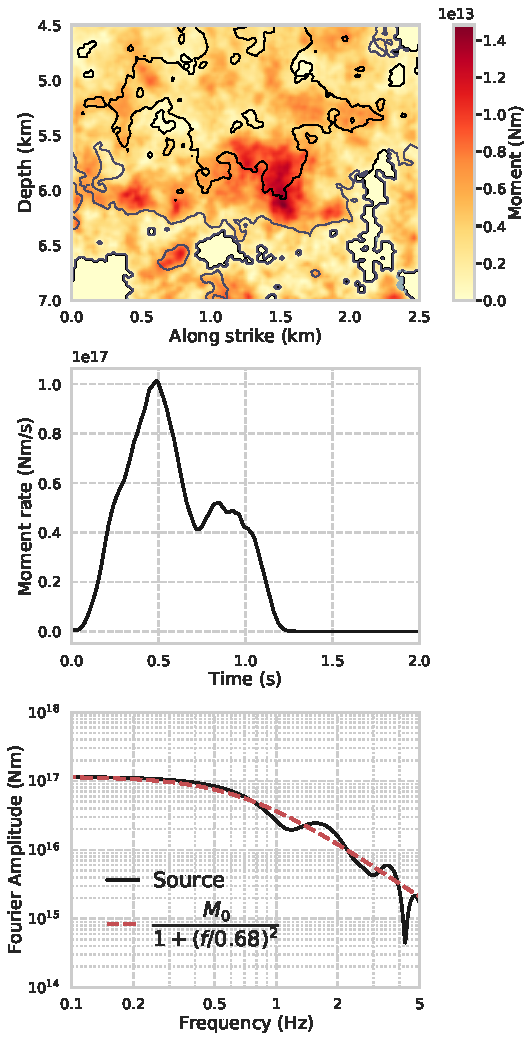
\includegraphics[width=0.9\textwidth,height=0.9\textheight,keepaspectratio]{figures/figure_vs30_2.pdf}
  \caption{Description of the source model used in this study. (a) Total moment on the fault. The contours represent rupture time at a 0.4 s interval starting from 0. (b) and (c) represent the sum of the moment rates for all subfaults and the Fouerier amplitude spectrum, respectively.}
  \label{fig:vs30-2}
\end{figure}

\clearpage
\begin{figure}[!ht]
  \centering
  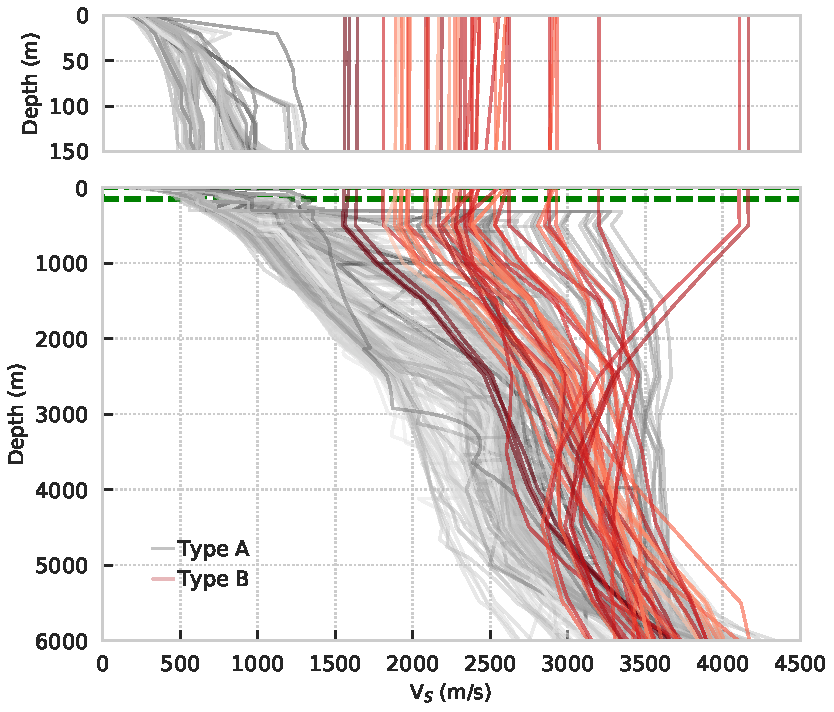
\includegraphics[width=0.9\textwidth]{figures/figure_vs30_3.pdf}
  \caption{(a) Top 150 m and (b) 0-4000 m $V_S$ profiles at the 259 stations. The black and red curves represent type B (surface $V_S$ >= 1000 m/s) and soil (surface $V_S$ < 1000 m/s) sites, respectively. The darker curves denote the sites with farther distance from the source.}
  \label{fig:vs30-3}
\end{figure}

\clearpage
\begin{figure}[!ht]
  \centering
  \includegraphics[width=0.9\textwidth]{figures/figure_vs30_4.pdf}
  \caption{FAS derived from the records (black) and CVM-S (blue) for the (a) east-west component, (b) north-south component and (c) vertical component. The left and right columns represent type A and B sites, respectively. The solid line is the median of FAS over the site group, the narrow band is the 95\% confidence interval of the median, and the dashed lines depict the standard deviation centered at the median.
  }
  \label{fig:vs30-4}
\end{figure}

\clearpage
\begin{figure}[!ht]
  \centering
  \includegraphics[width=0.9\textwidth]{figures/figure_vs30_5.png}
  \caption{(a) Surface $V_S$ extracted from CVM-S, and (b) $V_{S30}$ from \citet{thompsonUpdatedVs30Map2018} in our model domain (values in the left bottom corner are not available). The star denotes the epicenter.}
  \label{fig:vs30-5}
\end{figure}

\clearpage
\begin{figure}[!ht]
  \centering
  \includegraphics[width=0.9\textwidth]{figures/figure_vs30_6.pdf}
  \caption{Representative $V_S$ profiles for (a) type A sites and (b) type B sites from CVM-S. The thick black curves depict the averaged velocity profiles for all 220 type A and 39 type B sites directly extracted from CVM-S. The thin lines show the $V_S$ profiles resulting from our proposed method for different $z_T$ depths between 200 m and 1500 m. The dashed curve shows the $V_S$ profile calculated using the \Cref{eq:vs30-2} tapers from our preferred $z_T$ of 1000 m (note that because the tapers are applied as upper bounds to $V_S$, they typically only affect the type A $V_S$ structure at depths exceeding 350m, where the GTL in CVM-S ceases and causes the abrupt discontinuity).}
  \label{fig:vs30-6}
\end{figure}

\clearpage
\begin{figure}[!ht]
  \centering
  \includegraphics[width=0.9\textwidth]{figures/figure_vs30_7.pdf}
  \caption{The SH1D response for the refined profiles using various $z_T$ depths for average (a) type A and (b) type B sites, divided by the response obtained with the averaged type A and type B profiles from CVM-S.}
  \label{fig:vs30-7}
\end{figure}

\clearpage
\begin{figure}[!ht]
  \centering
  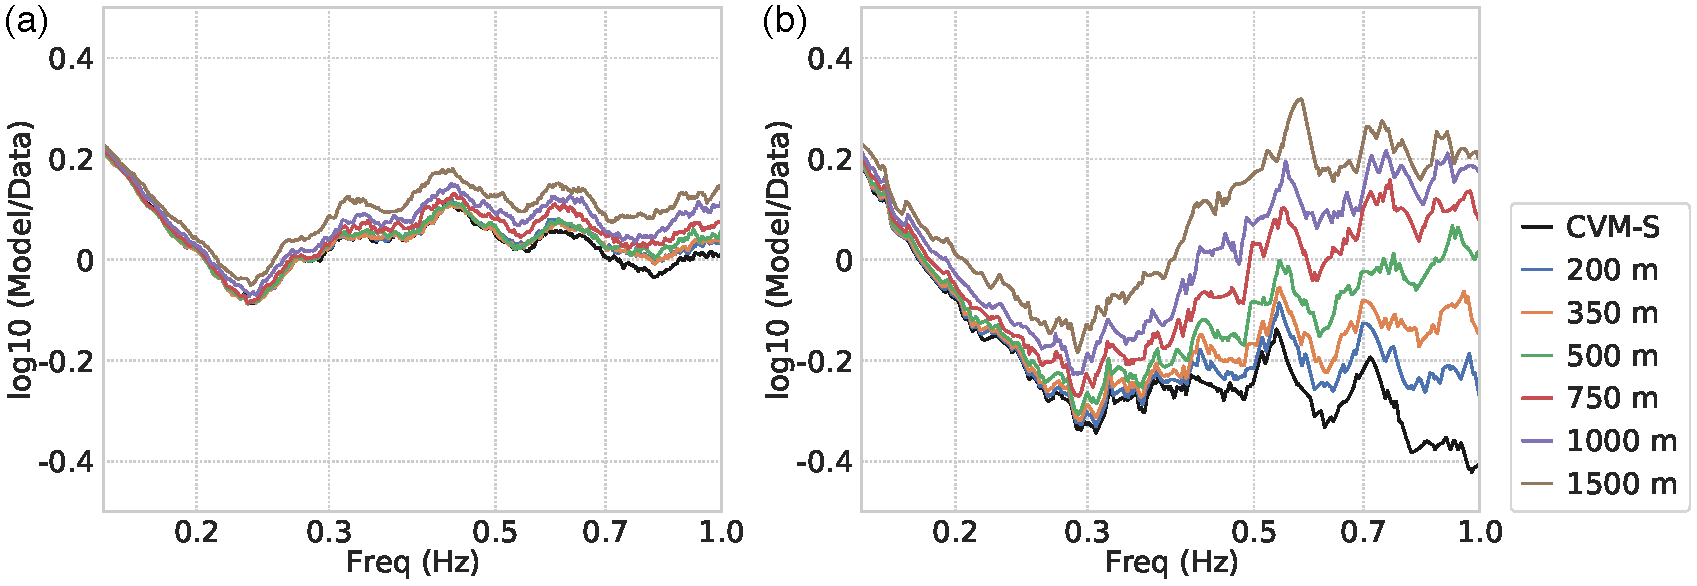
\includegraphics[width=0.9\textwidth]{figures/figure_vs30_8.pdf}
  \caption{Bias of FAS for the two horizontal components averaged over all (a) type A and (b) type B sites for CVM-S at all 259 stations, superimposed with the corresponding SH1D response. The black curves denote CVM-S and other labeled curves represent various tapering depths using SH1D results.}
  \label{fig:vs30-8}
\end{figure}

\clearpage
\begin{figure}[!ht]
  \centering
  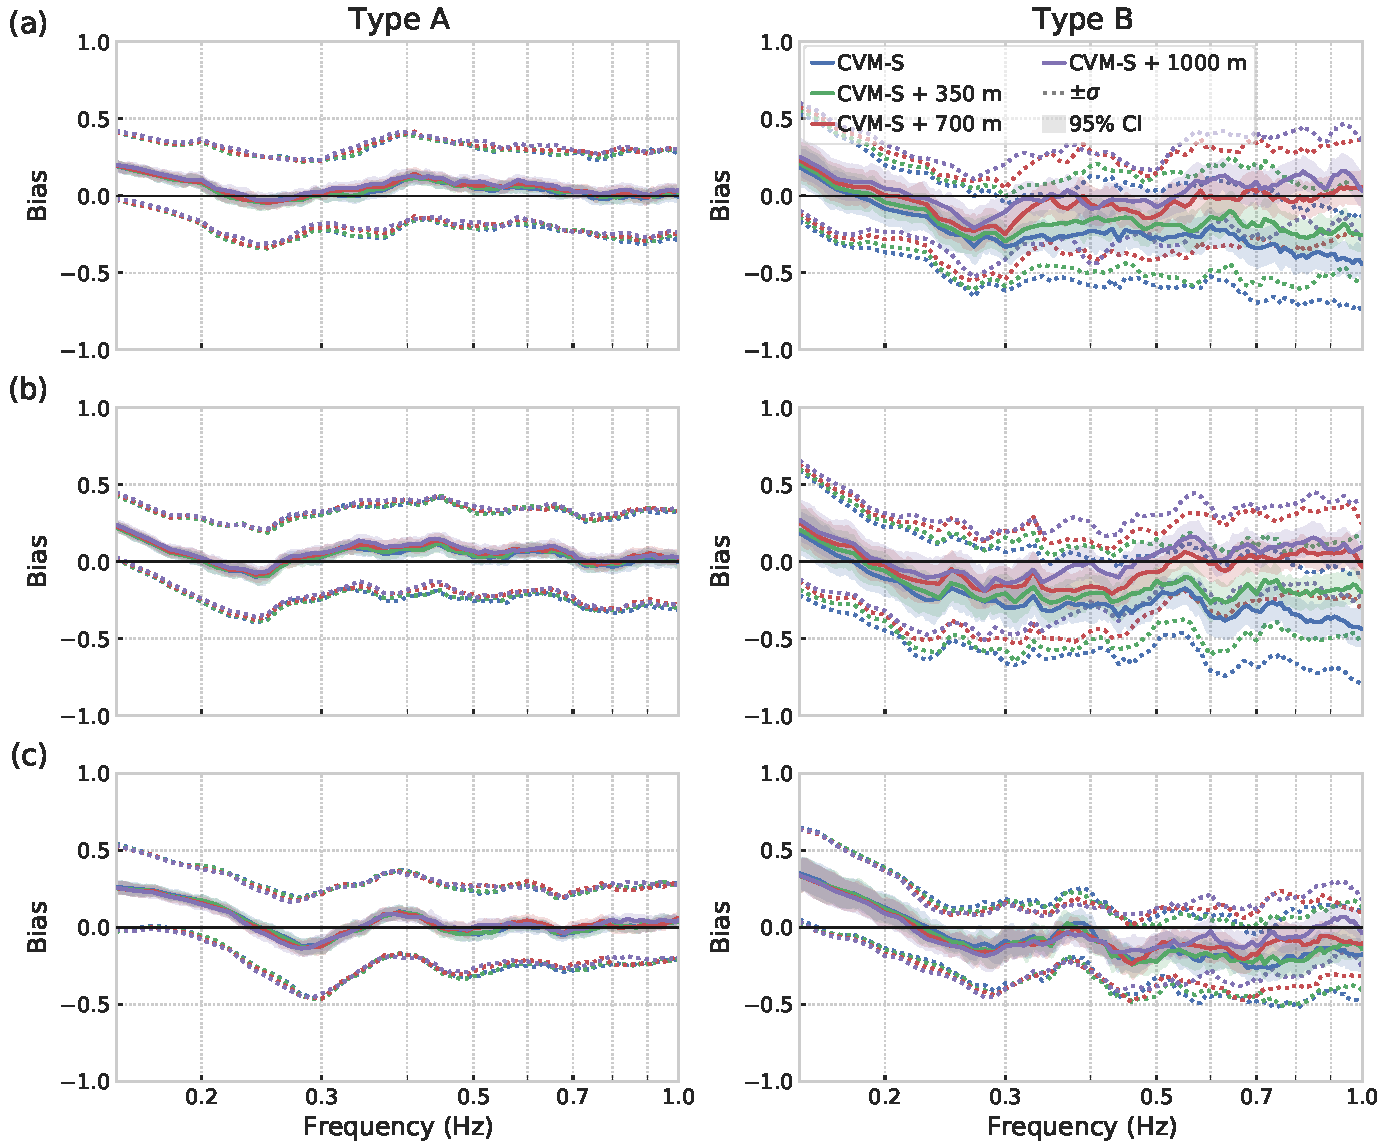
\includegraphics[width=0.9\textwidth]{figures/figure_vs30_9.pdf}
  \caption{Bias of FAS on the (a) east-west, (b) north-south and (c) vertical components, calculated from 3D simulations in CVM-S and with tapering depth of 350 m, 700 m, and 1000 m. A positive (negative) value depicts overprediction (underprediction). The left (right) column shows type A (B) sites. The solid line is the median of FAS, where the narrow band is the 95\% confidence interval of the median, and the dashed lines depict the standard deviation centered at the median.}
  \label{fig:vs30-9}
\end{figure}

\clearpage
\begin{figure}[!ht]
  \centering
  \includegraphics[width=0.9\textwidth]{figures/figure_vs30_10.png}
  \caption{Maps of interpolated log10-based FAS bias between four 3D models and data: (a) CVM-S, and CVM-S with tapering depth of (b) 350 m, (c) 700 m and (d) 1000 m, calculated from the synthetics and records at 259 stations. The warm (cool) colors represent overprediction (underprediction). The circles (triangles) depict type A (B) sites. Note the log10-based colorbar.}
  \label{fig:vs30-10}
\end{figure}

\clearpage
\begin{figure}[!ht]
  \centering
  \includegraphics[width=0.9\textwidth]{figures/figure_vs30_11.png}
  \caption{Maps of interpolated log10-based FAS bias for two 3D CVMs and data. (a) CVM-S with velocity tapering depth of 350 m and $Q_S=0.15V_S$, and (b) CVM-S with velocity tapering depth of 1000 m and $Q_S=0.05V_S$. Warm (cool) colors represent overprediction (underprediction). Circles depict type A sites and triangles show type B sites.}
  \label{fig:vs30-11}
\end{figure}

\clearpage
\begin{figure}[!ht]
  \centering
  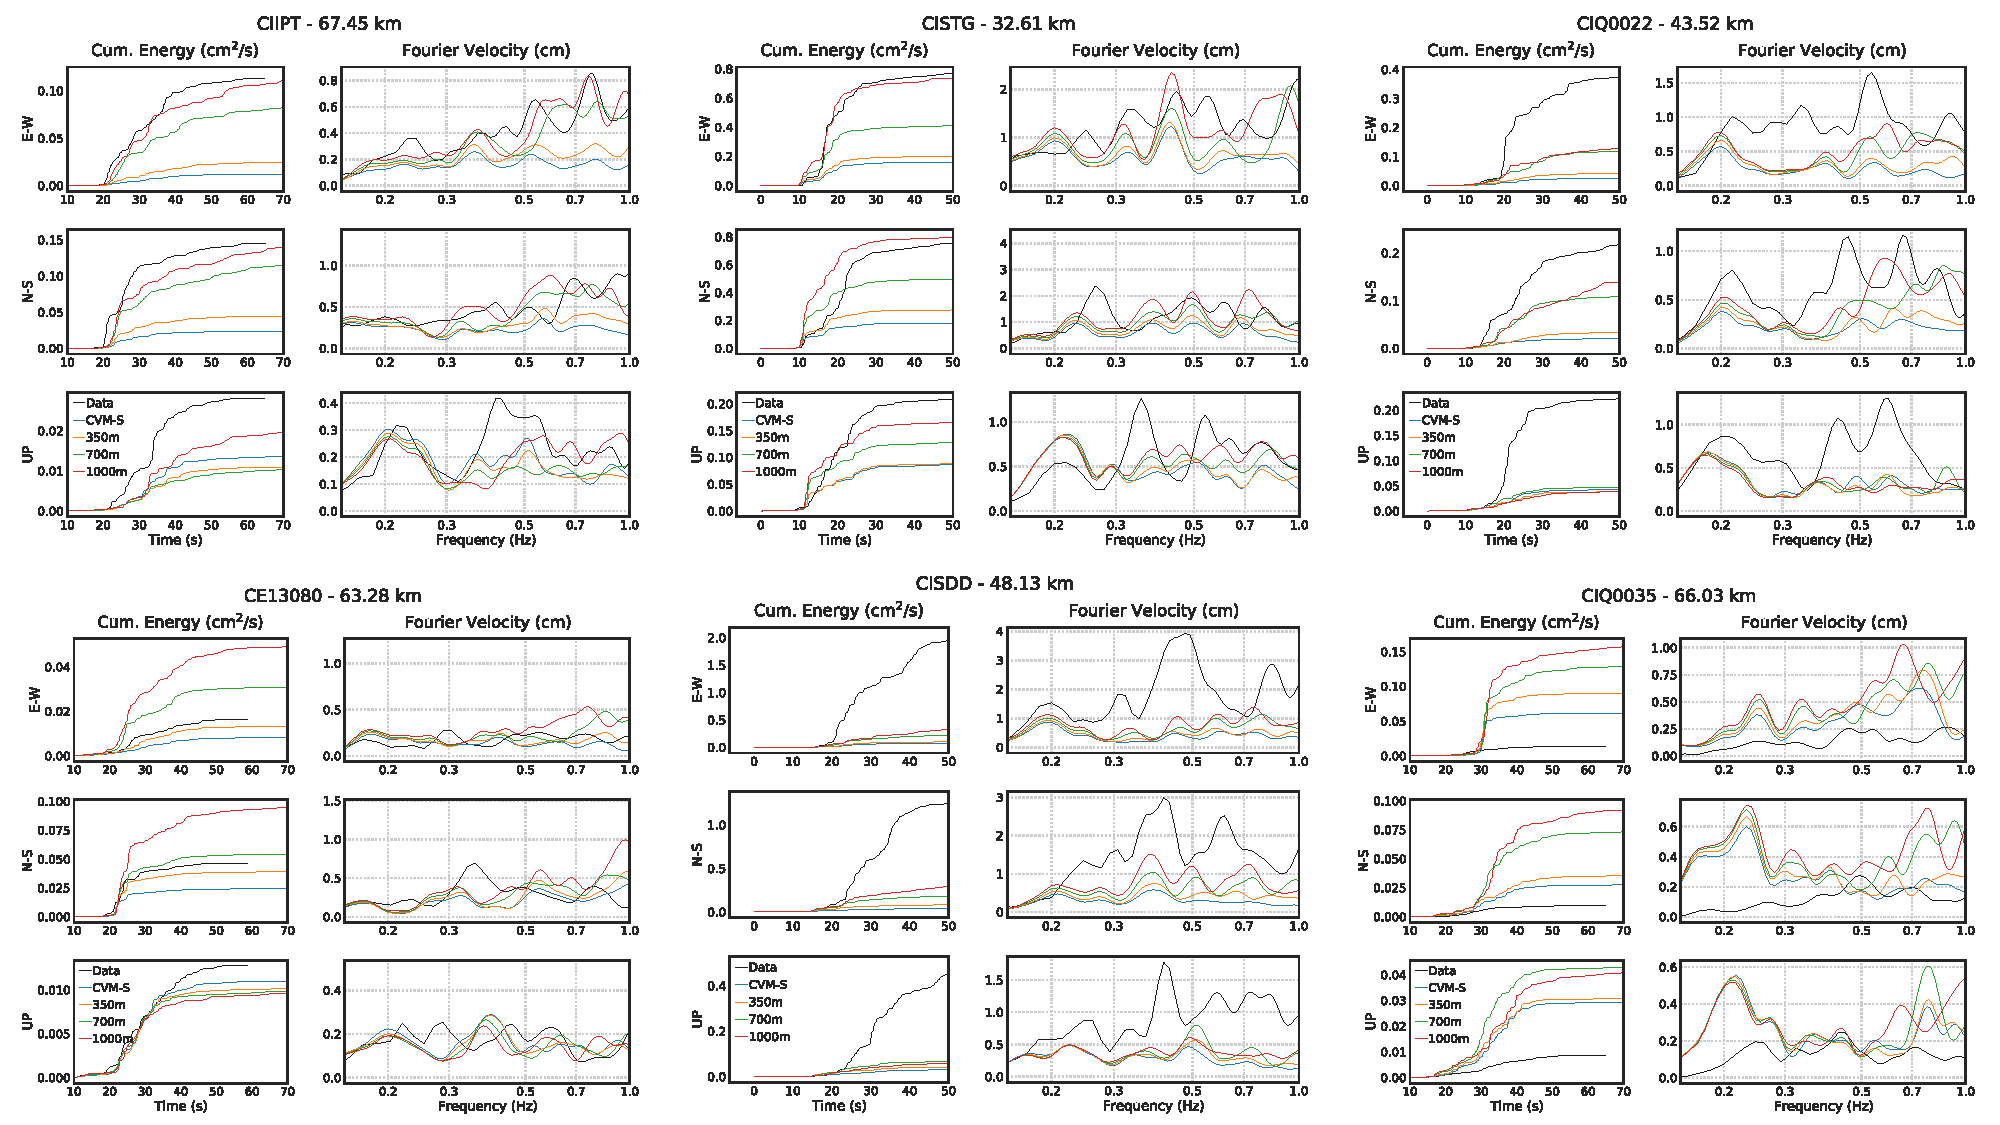
\includegraphics[width=0.9\textwidth]{figures/figure_vs30_12.pdf}
  \caption{Cumulative kinetic energy and Fourier velocity spectra at six type B sites. The subtitles show the names of the sites and their hypocentral distance.
  }
  \label{fig:vs30-12}
\end{figure}

\clearpage
\begin{figure}[!ht]
  \centering
  \includegraphics[width=0.9\textwidth]{figures/figure_vs30_13.pdf}
  \caption{Type B site $V_S$ profiles from CVM-S, and CVM-S and CVM-H with (default) \citet{elyVs30derivedNearsurfaceSeismic2010} GTL refinement depth of 350 m.}
  \label{fig:vs30-13}
\end{figure}

\clearpage
\floatsetup[figure]{style=plain,subcapbesideposition=top}
\begin{figure}[!ht]
  \sidesubfloat[]{\includegraphics[width=0.4\textwidth]{figures/figure_vs30_14a.png}\label{fig:vs30-14a}} \hfil
  \sidesubfloat[]{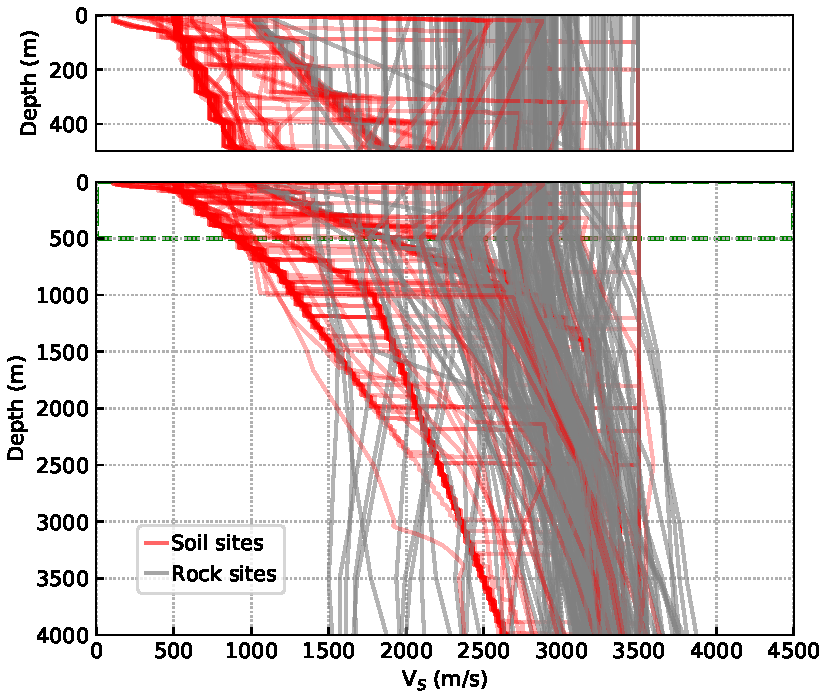
\includegraphics[width=0.45\textwidth]{figures/figure_vs30_14b.pdf}\label{fig:vs30-14b}} % \\[\baselineskip]%
  \caption{ (a) $V_S$ profile sample locations in California. Triangles denote type B sites and circles denote type A sites, and (b) extracted $V_S$ profiles. The top panel zooms into the top 500 m. }
  \label{fig:vs30-14}
\end{figure}


%% supplement
\setcounter{table}{0}
\setcounter{figure}{0}
\numberwithin{figure}{chapter}
\numberwithin{table}{chapter}
\renewcommand{\thetable}{S\arabic{chapter}.\arabic{table}}
\renewcommand{\thefigure}{S\arabic{chapter}.\arabic{figure}}
\newpage
\section*{Supplementary Materials}
\addcontentsline{toc}{section}{\protect\numberline{}Supplementary Materials}

\begin{figure}[!ht]
  \centering
  \includegraphics[width=0.9\textwidth]{figures/figure_vs30_S1.pdf}
  \caption{Bias of FAS of the (a) east-west, (b) north-south and (c) vertical component, calculated from 3D simulations in CVM-S with minimum $V_S$ of 200 m/s (blue) and 500 m/s (green). A positive (negative) value means overprediction (underprediction). The left (right) columns show type A (B) sites. The solid line is the median of FAS, where the narrow band is the 95\% confidence interval of the median, and the dashed lines depict the standard deviation centered at the median.}
  \label{fig:vs30-S1}
\end{figure}
\clearpage

\begin{figure}[!ht]
  \centering
  \includegraphics[width=0.9\textwidth]{figures/figure_vs30_S2.pdf}
  \caption{Bias of FAS of the (a) east-west, (b) north-south and (c) vertical component, calculated from 3D simulations in CVM-S with $V_S$ tapering depths of 350 m and 1000 m along with attenuation models $Q_S=0.05V_S$, $Q_S=0.1V_S$, and $Q_S=0.15V_S$. A positive (negative) value means overprediction (underprediction). The left (right) columns show type A (B) sites. The solid line is the median of FAS, where the narrow band is the 95\% confidence interval of the median, and the dashed lines depict the standard deviation centered at the median.}
  \label{fig:vs30-S2}
\end{figure}
\clearpage

\begin{figure}[!ht]
  \centering
  \includegraphics[width=0.9\textwidth]{figures/figure_vs30_S3.pdf}
  \caption{Averaged FAS bias for frequencies between 0.15-1 Hz at poorly constrained sites plotted as a function of site surface $V_S$ for (a) three-component average, (b) east-west, (c) north-south and (d) vertical components. The shades represent 95\% confidence intervals estimated using bootstrap.}
  \label{fig:vs30-S3}
\end{figure}


\renewcommand{\thetable}{\arabic{table}}
\renewcommand{\thefigure}{\arabic{figure}}

\numberwithin{figure}{chapter}
\numberwithin{table}{chapter}

%\endrefsection
% !TEX encoding = UTF-8 Unicode

\linespread{1.7}
\chapter{Modeling of Empirical Transfer Functions with 3D Velocity Structure}
\linespread{2.0}
%\newrefsection
\label{chap:etf}

Empirical transfer functions (ETFs) between seismic records observed at the surface and depth represent a
powerful tool to estimate site effects for earthquake hazard analysis. However, conventional modeling of
site amplification, with assumptions of horizontally polarized shear waves propagating vertically through
1D layered homogeneous media, often poorly predicts the ETFs, particularly, in which large lateral variations
of velocity are present. Here, we test whether more accurate site effects can be obtained from theoretical
transfer functions (TTFs) extracted from physics-based simulations that naturally incorporate the complex
material properties. We select two well-documented downhole sites (the KiK-net site TKCH05 in Japan and
the Garner Valley site, Garner Valley Downhole Array, in southern California) for our study. The 3D subsurface
geometry at the two sites is estimated by means of the surface topography near the sites and information
from the shear-wave profiles obtained from borehole logs. By comparing the TTFs to ETFs at the selected sites,
we show how simulations using the calibrated 3D models can significantly improve site amplification estimates
as compared to 1D model predictions. The primary reason for this improvement in 3D models is redirection of
scattering from vertically propagating to more realistic obliquely propagating waves, which alleviates
artificial amplification at nodes in the vertical-incidence response of corresponding 1D approximations,
resulting in improvement of site effect estimation. The results demonstrate the importance of reliable
calibration of subsurface structure and material properties in site response studies.

%%%%%%%%%%%%%%%%%%%%%%%%%%
\section{Introduction} \label{etf:intro}
Details of how ground shaking is affected by near-surface soil properties can help reduce the uncertainty in stochastic or empirical ground-motion models, which are important components of seismic hazard calculations. Transfer functions (TFs) are widely used to quantitatively represent site response by computing the spectral ratio of ground motions between site and reference locations in the frequency domain \citeg{shearerSurfaceNearsurfaceEffects1987,steidlVariationSiteResponse1993,fieldComparisonTestVarious1995,steidlWhatReferenceSite1996,bonillaBoreholeResponseStudies2002}. Assuming that the reference site, while sharing, approximately, the same path and source with the site of interest, is largely unaffected by site effects,the spectral ratio provided by the TF isolates the site response \citep{borcherdtEffectsLocalGeology1970}. Two types of reference sites, both typically rock, have been proposed: a surface site or a downhole recording (used with the corresponding surface site). The surface downhole record pair is valuable for ensuring close proximity of the reference motions at the downhole sensor, ideally located in bedrock, whereas, it may be difficult to find an appropriate reference outcrop site within close distance to the soil site. In this article, we will only analyze TFs computed using surface-downhole site pairs.

The accuracy of site response estimates depends on the accuracy of the subsurface model used, and this is usually assumed to be controlled by the uncertainty in the site properties, in particular, the shear-wave velocity, $V_S$ \citeg{baraniInfluenceSoilModeling2013,griffithsMappingDispersionMisfit2016}. $V_s$ is the most important parameter for conventional 1D modeling of the TF, in which it is assumed that surface (and subsurface) motion consists of horizontally polarized plane S waves propagating through a stack of homogeneous layers \citeg{kramerGeotechnicalEarthquakeEngineering1996}. This modeling procedure (SH1D) ignores the lateral complexity of the often heterogeneous geology and subsurface structure and is, therefore, not able to include potential 2D and 3D amplification effects in the observations \citeg{rotenComparisonObservedSimulated2008,thompsonTaxonomySiteResponse2012}. \citet{zhuSeismicAggravationShallow2018} performed numerical analysis on 2D basins and found that a constant spectral aggravation factor \citep{chavez-garciaComplexSiteEffects2000}, which quantifies the discrepancy between 1D and 2D/3D models, is insufficient to identify basin effects, especially, in close-to-edge regions of shallow basins. Both observations and analytical solutions suggest that 1D models lack an estimate of spatial variability, caused by complex wave propagation such as basin amplification, surface-wave generation, and scattering, and are, therefore, unable to capture spatial correlations, which may be important for understanding risk, especially, to regional-scale infrastructure \citeg{olsenCausesLowfrequencyGround1995,booreCanSiteResponse2004}. Although, recent approaches have attempted to reduce velocity uncertainties in site effect estimation \citep{matavosicPracticesProceduresSitespecific2012,teagueMeasuredVsPredicted2018}, these methods either require prohibitively complex processing or are developed for specific cases only.

It is impractical to constrain subsurface structure over a wide region to the resolution (on the order of meters to tens of meters) required for accurate ground-motion estimation to high frequencies (e.g., 10 Hz). Instead, some studies choose to use simple proxies, based on broad site classes to supplement estimates of soil properties and site spatial characteristics, for example, the National Earthquake Hazards Reduction Program (NEHRP) soil classification \citep{bssc2003NEHRPRecommended2003,akkarEmpiricalEquationsPrediction2010} or a weighted average of $V_S$ in the uppermost 30 m \citep[$V_{S30}$, e.g., ][]{abrahamsonSummaryAbrahamsonSilva2008,idrissNGAWest2EmpiricalModel2014}. \citet{thompsonTaxonomySiteResponse2012} proposed a scheme to classify surface-downhole site pairs by the extent of interevent variability and goodness of fit between 1D modelling and empirical site response, which can be used to calibrate the constitutive models and guide specific site studies. Despite the use of these characterizations in some generic seismic hazard estimates, for instance, via ground-motion prediction equations, recent work has pointed out the importance of considering site-to-site amplification variability \citep{atkinsonEarthquakeGroundmotionPrediction2006,atikVariabilityGroundmotionPrediction2010}. These studies show that, even within a single NEHRP or $V_{S30}$ class, the variability of site amplification and spatial correlations is strong enough to contribute significant uncertainty in ground-motion estimates.

In this chapter, we propose a method to constrain the near-surface properties using surface topography and perform high-resolution 3D numerical simulations to investigate the uncertainty in site response modeling. The simulations naturally take advantage of 3D geotechnical information and are able to incorporate complicated spatially varying amplification effects. We use two downhole array sites, namely the Garner Valley Downhole Array (GVDA) in California and the TKCH05 site from the Kiban–Kyoshin network (KiK-net) surface-downhole pairs in Japan, where detailed in situ constraints of site seismic properties (e.g., $V_S$ and layer thicknesses) and abundant earthquake records are available, for our analysis. Both borehole sites have well-documented geological structure data, and previous studies have showed that SH1D modeling poorly predicts the ground motions without adjustments of subsurface properties or recalibration of constitutive models. \citet{thompsonTaxonomySiteResponse2012} found low interevent variability and poor fit using SH1D modeling for the site TKCH05, due to omission of spatial variability around the site that scatters the downgoing waves and reduces pseudoresonance. They found that no satisfactory fit could be achieved by adjusting the velocity profile, whereas \citet{taoTaxonomyEvaluatingSitespecific2020} showed that modification in the top 20 m can significantly improve the site response estimate for the outcrop TF (spectral ratio between two surface sites). \citet{bonillaBoreholeResponseStudies2002} studied the wave propagation at GVDA and reported significant S-to-P conversions that led to misfit in prediction of the empirical TF (ETF; see \Cref{etf:tfs}) by horizontal-to-vertical spectral ratios. \citet{teagueMeasuredVsPredicted2018} applied the Toro randomization model \citep{toroProbabilisticModelsSite1995} with the spectral analysis of surface waves method, to obtain the site signature with the best match of the ETF and the theoretical TF (TTF); however, this approach suffers from the nonunique nature of inverting $V_S$ profiles.


%%%%%%%%%%%%%%%%%%%%%%%%%%%%%%%
\section{Data}\label{etf:data}

Dependent on the strength of the input motion, site amplification and deamplification can be caused by a combination of linear and nonlinear effects. Here, we focus on linear site effects, and reserve the nonlinear analysis for subsequent research endeavors. To limit our analysis to linear ground motions, we exclude records with maximum surface accelerations larger than 0.1g \citeg{beresnevNonlinearSoilResponse1996}. For each of the two site selections, we randomly picked 36 events of various azimuth and distance to the site that meets this criterion, with a minimum signal-to-noise ratio of five in their records. The goodness of fit between TTFs and ETFs from recordings is described by the variance reduction (VR) as follows:
\begin{equation}\label{eq:etf-1}
  \mathrm{VR}=1-\frac{\sum_{i=1}^{n}\left[\operatorname{TTF}\left(f_{i}\right)-\mathrm{ETF}_{\mathrm{med}}\left(f_{i}\right)\right]^{2}}{\sum_{i=1}^{n}\left[\mathrm{ETF}_{\mathrm{med}}\left(f_{i}\right)\right]^{2}}
\end{equation}
\noindent in which $n$ is the number of frequencies at which the ETFs and TTFs are computed, and ETF med is the median of the ETFs from the events that we selected. We evaluate a set of linearly spaced frequencies between 0.5 and 10 Hz, with the lower limit determined by the noise level of the data, and the upper limit from the resolution of our simulations. The VR ranges within $[-\inf, 1]$, in which VR = 1 means a perfect match, and smaller values indicate poorer fit.

%%%%%%%%%%%%%%%%%%%%%%%%%%%%%%

\section{TFs}\label{etf:tfs}
We compute TFs between surface and downhole locations as follows:
\begin{equation}\label{eq:etf-2}
  TF = \frac{G_s(f)}{G_d(f)}
\end{equation}
\noindent in which $G_s(f)$ and $G_d(f)$ are the root mean squares of the Fourier amplitude spectra of horizontal accelerations at the surface and downhole locations, respectively. It is worthwhile to note that the downhole recordings include the upgoing incident wavefield as well as downgoing waves that are reflected back from the free surface. This phenomenon complicates the wavefields recorded at downhole sites, and, therefore, the use of surface-downhole pairs to study site response. For records obtained at depths shallower than 200 m, as in this study, the upgoing and downgoing pulses overlap in the records, with differences in arrival times as small as 0.2 s, complicating a separation of the two contributions in the presence of extended source duration and site response \citep{shearerSurfaceNearsurfaceEffects1987}. For example, \citet{bonillaBoreholeResponseStudies2002}  found from simulations at the GVDA site using the f-k method that the downgoing wave effect is predominant above the soil-bedrock interface and strongly degraded below that depth. Because it is almost impossible to eliminate downgoing waves from the records, we include the total wavefields at the surface and downhole sites, when calculating the TFs for both synthetics and records.

Our procedure for processing the recorded time series is similar to that documented in \citet{taoInsightsModelingSmallstrain2019}. First, we collected acceleration time series at the surface and downhole accelerometers. Second, a fifth-order Butterworth filter, with a passband of 0.5–12 Hz, was applied to the demeaned and detrended accelerations, in which signal at frequencies below 0.5 Hz was discarded to minimize the contribution from low-frequency noise interference. Third, a second-order polynomial baseline correction was applied to the observed displacement time series, obtained by integrating the accelerations twice. Then, the ETFs were obtained as the ratio of the Fourier spectral amplitude between the surface and downhole acceleration time series for all the events. We further smoothed the TFs using the Konno–Ohmachi smoothing window in the frequency domain \citep{konnoGroundmotionCharacteristicsEstimated1998}. Although, not necessary for the synthetics, we applied the preprocessing (steps 2 and 3) to both synthetics and data for consistency.


\section{Model Construction}\label{etf:model}
It is reasonable to assume that, in the vicinity of a site of interest, bedrock depth varies in accordance with surface topography. In such models, sites located in a mountainous area have near-zero bedrock depth, whereas, sites in valley regions are characterized by larger depths to bedrock. Under this assumption, our 3D mesh is generated by mapping the topography to bedrock depth, with the constraints from borehole logging measurements. Oftentimes, bedrock depth increases
rapidly from the edge toward the center of a sedimentary valley and approaches a maximum near the center of the valley, suggesting that depth to bedrock in a valley can be estimated using the topographic signature from digital elevation models. \citet{gallantMultiresolutionIndexValley2003} proposed an algorithm that operates at multiple scales and combines topographic elevations into a single continuous multiresolution index of valley bottom flatness (MRVBF). Values of MRVBF below 0.5 represent areas with the steepest topography, values between 0.5 and 1.5 relate to the steep areas with few flat valley bottoms, and larger MRVBF values indicate broader and flatter valley bottoms. Here, we adopt the MRVBF technique and used the same threshold value (1.5) as in \citet{gallantMultiresolutionIndexValley2003}, to discriminate valley and mountainous regions. The quantitative relationship between the bedrock depth (D) and MRVBF values are assumed to obey a logarithmic formula:
\begin{equation}\label{eq:etf-3}
  D = max(0,\quad D_0 * log_{10}(\frac{MRVBF}{MRVBF_t}))
\end{equation}
\noindent in which $MRVBF_t$ is the threshold MRVBF value (here, 1.5), and $D_0$ is a coefficient, which is calculated by substituting the MRVBF value and bedrock depth at the borehole site into the borehole equation, that is, $D_0=D_{borehole}/log_{10}(\frac{MRVBF_{borehole}}{MRVBF_t})$.

In addition to the modifications of the velocity model from the MRVBF method, we explore the extent to which scattering effects from statistical distributions of near-surface small-scale heterogeneities (SSHs) can improve site effect estimation. Previous studies using 1D modeling show that including SSHs may improve the prediction of ETFs, likely by weakening the downgoing wave effects \citep{nourFiniteElementModel2003,thompsonTaxonomySiteResponse2012}. Here, we use guidance from published studies on spectral coloring of Gaussian random numbers with von Karman spatial correlation functions for characterizing the statistics of heterogeneities \citep[see \cref{app:A}; as well as, e.g.,][]{frankelFiniteDifferenceSimulations1986,withersGroundMotionIntraevent2019}. We use a Hurst number of 0.05, a correlation length of 100 m, a standard deviation of 5\%, and a horizontal-to-vertical anisotropy of five, as constrained from sonic borehole logs in the Los Angeles basin by \citet{savranModelSmallscaleCrustal2016}. We include SSHs with these parameters, when generating TFs at our two selected locations, whereas, the sensitivity of the TFs to variation in the parameters is explored in the Discussion section.

\subsection{Numerical simulations}
Our goal to quantify the effects of 3D Earth structure on highfrequency (<10 Hz) TFs, using 3D modeling, is computationally challenging. We use the parallel and scalable discontinuous-mesh velocity–stress staggered-grid finite-difference code AWP-ODC-DM \citep{olsenSimulationThreeDimensional1994,cuiScalableEarthquakeSimulation2010,nieFourthOrderStaggered2017} to simulate the site response. One-dimensional TTFs are computed under the SH1D assumption, in which the model consists of a stack of homogeneous layers, to provide a point of comparison for the 3D models. The model definition for the 3D TTF computation is more complicated. We include the effects of frequency-dependent attenuation using the model:
\begin{equation}
  Q(f) =
  \begin{cases}
    Q_0 \times f_\gamma, & f > 1   \\
    Q_0,                 & f \le 1
    \label{eq:etf-4}
  \end{cases}
\end{equation}

\noindent in which $Q_0$ is a frequency-independent constant attenuation proportional to the velocity, and $\gamma$ is a power-law exponent describing the attenuation above 1 Hz \citep{withersMemoryEfficientSimulation2015}. Here, we adopt area-specific parameters suggested in the literature; for GVDA, we use $Q_{S,0}=0.05 \times V_S$ ($V_S$ in meters per second), $Q_{P,0}=2 \times Q_{S,0}$ , and $\gamma=0.6$ \citep[for southern Calfornia]{withersMemoryEfficientSimulation2015}, and for TKCH05, we use a model for $Q_{P,0}=Q_{S,0}=Q_0$, given by
\begin{equation}
  Q_{0}=\left\{\begin{array}{ll}
    60,  & V_{S} \leq 600       \\
    100, & 600<V_{S} \leq 1100  \\
    150, & 1100<V_{S} \leq 2100 \\
    \label{eq:etf-5}
    200, & 2100<V_{S} \leq 3200 \\
    300, & V_{S}>3200
  \end{array}\right.
\end{equation}
\noindent in which $V_S$ is in meters per second, from the Japan Seismic Hazard Information Station (J-SHIS) and $\gamma=0.2$, following the study by \citet{nakajimaSeismicAttenuationNortheastern2013}. We discretize the velocity models using two partitions in our discontinuous mesh, with grid spacings small enough to resolve the minimum $V_S$ wavelengths (20 m and 14 m for the GVDA and TKCH05 cases, respectively), anywhere in the model with, at least, five points. In our simulations, the surface recordings at a neighboring outcrop site are deconvolved from its local subsurface property layers, up to the bottom of the simulation domain; the resulting three-component acceleration time series (converted to body forces in AWP-ODC-DM) are then distributed on the entire bottom surface of the computational domain, to generate a oneway upward propagating plane wave. We verified that such vertical-incident plane wave sources are reasonable approximations, considering our shallow simulation domains (0.4 km and 1 km deep at GVDA and TKCH05, respectively), as well as earthquake hypocenters at depths of 10 km+ and distances of tens of kilometers. We used an elastic boundary condition at the bottom grid boundary, which is transparent to downgoing waves, to avoid artificial resonance of the soil column \citep{roten3DSimulationsEarthquakes2012}. We part from the common way of placing the model base at the downhole site and have the input motion as the downhole motion, due to our boundary conditions. We perform the numerical simulations on the Oak Ridge National Laboratory Summit supercomputer, in which each of our simulations with the 3D model at TKCH05, including 64 million cells, requires a wall-clock time of 100 min on 32 graphic processing units for 750,000 timesteps. Similar computational requirements are needed for the 3D GVDA simulations.


\section{GVDA}\label{etf:gvda}
The GVDA is located in a seismically active region of California, 7 km from the San Jacinto fault and 35 km from the San Andreas fault \citep[see \cref{fig:etf-1};][]{archuletaGarnerValleyDownhole1992}. The site is situated in a narrow valley within the Peninsular Ranges Batholith \citep{bonillaBoreholeResponseStudies2002}, 23 km east of Hemet and 20 km southwest of Palm Springs, California. The near-surface stratigraphy beneath GVDA consists of extensive lake-bed alluvium and decomposed crystalline rocks \citep{hillGeologyGarnerValley1981}. Soft silty and clayey sands makes up the top 18–25 m across the site \citep{steidlWhatReferenceSite1996}, followed by 50–60 m thick, decomposed, and weathered granite down to about 64–87 m, as constrained by seismic downhole testing and shallow and deep P–S velocity suspension logging \citep{gibbsNearsurfaceSwaveVelocities1989,stellerNewBoreholeGeophysical1996}. The GVDA site is equipped with multiple downhole accelerometers, at depths of 15, 22, 50, and 150 m that are capable of measuring accelerations from $3 \times 10^{-6}$ to $2.0g$ below 100 Hz. The 150 m deep accelerometer is the only downhole sensor that penetrates the granitic rock, which is used to compute TTFs in this study.

To be able to resolve frequencies up to 10 Hz at the GVDA site, we generated a mesh of size 4 km × 4 km × 0.4 km (length × width × depth), with mesh properties compressional wave velocity ($V_P$), $V_S$ and density from the 3D Community Velocity Model (CVM) S4.26.M01, which is developed and maintained by the Southern California Earthquake Center \citep[SCEC;][]{smallSCECUnifiedCommunity2017}. The borehole logs show $V_S$ of the near-surface soft soils between 180 and 220 m/s, with the value of $V_S$ smaller than 200 m/s only at depths between 1.4 and 2.8 m \citep{stellerNewBoreholeGeophysical1996}. The minimum velocity in our model was truncated at 200 m/s, which is about the average of the top 4 m, resolving frequencies up to 10 Hz, with, at least, five points per minimum S wavelength, using a smallest grid spacing of 4 m. The SCEC CVM S4.26.M01, however, fails to resolve the 3D Garner Valley structure to the accuracy required by our analysis, and we use the MRVBF method to describe the depth to bedrock instead.

At every surface location, we first compute the MRVBF value and bedrock depth, as described in the Numerical simulations section. We then force the $V_P$, $V_S$ , and densities above the bedrock to be the same as those in the measured borehole log, while keeping the seismic velocities and densities unchanged in the bedrock. \Cref{fig:etf-2} illustrates how we estimate bedrock depth from the MRVBF values, using surface topography. The deeper parts of the valley are represented by larger MRVBF values. The areas with MRVBF smaller than the threshold value at 1.5 are shown in dark shading, corresponding to steeper terrain. The borehole site GVDA, at the center of the region, has a MRVBF value of 5.8 and bedrock depth of 64 m, consistent with the borehole log from \citet{gibbsNearsurfaceSwaveVelocities1989}. The 3D geometry inferred from the spatially varying bedrock depth is shown in the left panels of \Cref{fig:etf-3}, compared to the original borehole profile in the right panel.

Although we computed the ETFs for all the selected 36 events (\cref{tb:etf-1,fig:etf-A1}), only one event (ID = 33) was used to generate the upgoing waves in the simulations and to compute the TTF. The selection of event ID 33 was arbitrary for two reasons: (1) the ETFs at GVDA show low interevent source variability, indicated by the narrow $\rm \sigma$ band in \Cref{fig:etf-4}, and (2) the modeling is constrained to linear wave propagation. The use of a realistic source allows straightforward extension to multiple sites, as well as to nonlinear analysis in the future. The source time function was obtained by deconvolving the surface recordings of this event at the neighboring outcrop site GVAR (see \cref{fig:etf-1}) to the maximum depth of our domain.

The TTFs and ETFs for GVDA are compared in \Cref{fig:etf-4}. The two-sigma scatter of all the ETFs is fairly narrow above 1 Hz and not sensitive to the azimuths and distances of the events, which implies that the ETFs are primarily determined by the site characteristics, and confers greater predictive power on an ETF (and presumably also on a TTF). Although the peaks for the ETFs and both 3D and 1D TTFs generally occur near the same frequencies, the goodness of fit predicted from the 1D model (VR = 0.64) is significantly smaller compared to the 3D model (VR = 0.85). This result suggests that the shallow 3D structure contributes first-order effects to the local site amplification at GVDA (see \cref{etf:discussion}).

\section{TKCH05}\label{etf:tkch05}
The KiK-net strong-motion seismograph network in Japan provides, approximately, 700 sites, with pairs of surface and downhole seismographs installed that have recorded earthquakes with a wide range of magnitudes. KiK-net also provides geological and geophysical data, including velocity structure for each site, derived from borehole logs. \citet{thompsonTaxonomySiteResponse2012} analyzed the interevent variability and goodness of fit between SH1D models and data at 100 sites from KiK-net, and identified some sites where the standard 1D site response analysis provided poor results. Among these sites, we targeted TKCH05, which is located in Honbetsu, Hokkaido, Japan, to investigate the contributions from its underlying 3D structure on site effects. \Cref{fig:etf-5} shows the location of TKCH05, in a narrow valley surrounded by mountains. The large gradients of the surface topography at the valley boundaries suggest the presence of significant 3D variation of the bedrock interface below the valley. The stratigraphy at TKCH05 is, approximately, 6 m of soil and sandy gravel with $V_S$ = 140 m/s, overlying tens of meters of sandstone over gravel stone and siltstone \citep[see \cref{fig:etf-6};][]{nationalresearchinstituteforearthscienceanddisasterresilienceNIEDKNETKiKnet2019}. \Cref{tb:etf-2} lists the events included in our analysis of the ETFs at TKCH05 (see \cref{fig:etf-A2} for their locations and time series), among which the event with an ID of 1 was selected to generate the incoming waves in our simulations. As we did at site GVDA, we deconvolved the surface records at the closest outcrop site, F-net site URH, which is about 21.7 km away from TKCH05 to the domain bottom.

\Cref{fig:etf-6} shows the downhole profile at TKCH05, and Figure 7a shows a comparison between the corresponding 1D TTF compared to the ETFs. The 1D TTF fails to match the frequency peaks and strongly overpredicts the amplifications at lower frequencies, producing a relatively low VR (VR = 0.35). We also considered the adjacent K-Net site HKD090, due to its proximity to TKCH05 (only 4 m relative distance), in our analysis. The available information from the measured $V_S$ profile at HKD090 only extends to a depth of about 18 m, but, varies notably from those at TKCH05, considering the close distance. Because the top layers are as thin as 2 m, it is possible that the accuracy was degraded when the downhole logging measurements of travel time were converted to piecewise constant profiles. For this reason, we tested a simplified profile combining the two borehole logs, by replacing the TKCH05 $V_S$ profile between 5 and 100 m, with an average value of 680 m/s. The adjustment reduces the strong discrepancy in shallow $V_S$ values between the two borehole logs and retains the travel time from the bedrock to the surface. The SH1D model with the simplified profile produces a poorer fit to the ETF (VR = 0.181) than that obtained using the TKCH05 profile. Although, the simplified profile agrees better with the location of the second spectral peak of the ETF, the overall response compares less favorably to that obtained using the original profile due to larger amplitudes, especially at frequencies between 1 and 3 Hz.

Next, we extract our background 3D models at TKCH05 with a 1 km × 1 km × 1 km region, with the top boundary centered at TKCH05, from the Japanese national subsurface $V_S$ model provided by J-SHIS. The J-SHIS model provides $V_S$ and $V_P$ and density with a horizontal spatial resolution of 1 km. Along the vertical direction, J-SHIS provides the depths of 33 layers with various thicknesses. Each layer is homogeneous and of increasing $V_S$ with depth, ranging from 350 to 3400 m/s. Given the coarse horizontal resolution, the J-SHIS model is essentially 1D, with small stepwise discontinuities present close to the southern edge of the model (\cref{fig:etf-8}d). The bedrock depth was then estimated using the MRVBF method. The $V_S$ below the downhole array is 1100 m/s, which increases to 1700 m/s at the bottom of our domain (\cref{fig:etf-8}). Based on the surface $V_S$ of 140 m/s, we interpolated the initial mesh to a grid spacing of $\Delta{h}$ = 2.5 m in the top partition of the mesh, to ensure at least 5–6 points per minimum S wavelength. In the discontinuous mesh setup, the lower mesh partition starts at a depth of 400 m, with a grid spacing of 7.5 m. \Cref{fig:etf-7}a compares ETFs to TTFs, based on the 3D models generated by the MRVBF technique, as well as the soil profile at TKCH05 and our simplified profile. Compared to the 1D models, the 3D models are able to fit the ETFs much better, with VR values of 0.50 and 0.86 for the 3D models with the original and simplified profiles, respectively. The 3D models, while both producing a shift of the second peak compared with their corresponding 1D models, show remarkable improvement in the amplitudes of the first peak, especially when using the simplified profile. The results suggest that the simplified velocity profile, combining the borehole logs from the two adjacent sites, characterizes the local subsurface velocity structure below TKCH05 significantly better than the TKCH05 borehole log.

In general, a site response model can be evaluated by comparing the predicted surface ground motions (obtained by convolving the TF with the records at the reference site), with those recorded at the site of interest. We follow the traditional procedure for the calculation of TFs, neglecting the phase in the convolution process and quantifying the goodness of fit by the amplitudes only. \Cref{fig:etf-7}b,c compares the 1.5-8 Hz band-pass filtered surface recordings to the predicted motions from TTFs, illustrating the improvement in synthetic waveforms, as compared to data obtained at TKCH05 using the 3D as compared to the 1D model.

\section{Discussion}\label{etf:discussion}
We have demonstrated for two borehole sites (GVDA and TKCH05) that site amplification estimation using TTFs can be significantly improved by including effects of the underlying 3D structure. However, the 3D TTFs still leave some room for improvement. A likely important cause of the remaining misfit between TTFs computed using 3D structure and the ETFs is the uncertainty in seismic velocity estimates as a function of depth. It is common practice in soil analysis to approximate the near-surface geology as a stack of layers with constant velocity. \citet{booreUsingSurfacesourceDownholereceiver2007} showed that the effects of approximating logging measurements with 10 m thick, constant-slowness layers are small for frequencies less than about 5 Hz. However, \citet{dayRMSResponseOnedimensional1996} examined analytically the relation between site response in the frequency domain and elastic structure and found that the spectral average of bandwidth ${\Delta{f}}$ is only constrained by the elastic structure up to a two-way travel-time depth of ${1/\Delta{f}}$. This means that the average TF (predominantly at higher frequencies) can be biased due to uncertainty in the shallow structure. Because the first layer is often thin, a bias in the thickness estimate can contribute relatively large error in the site effects.

The deeper structure, in particular, the bedrock depth, can also be important in determining the TFs. In conventional 1D models, the bedrock topography is simplified as a layer with fixed depth; whereas, our approach incorporates lateral variations by mapping surface topography. The subsurface structure in our model is, therefore, composed of multiple irregular interfaces, each of which is anchored to the borehole log right beneath the site of interest. In some cases, the exact depth of the soil-bedrock interface is unclear. For example, the weathered granite boundary below the GVDA site is reported at 64 m by \citet{gibbsNearsurfaceSwaveVelocities1989} and 87 m by Steller \citet{stellerNewBoreholeGeophysical1996}. The two velocity profiles are similar, except for the bedrock depth (\cref{fig:etf-9}a). In the following discussion, the two models utilize their respective bedrock depth and velocity profiles. \Cref{fig:etf-9}b shows the TFs from two 3D models assembled with the Gibbs and Steller profiles (the latter shifted 1 m deeper than the reported value due to the 4 m spatial resolution of our model). The Steller model response matches the ETF at high frequencies better than that from the Gibbs model, whereas, the latter model fits better at 1.5–7 Hz, with a slightly better overall fit (VR = 0.85 vs. 0.82). It is noticeable that the Steller model, representing lower average velocity in the soil column, results in a shift of the peaks of the TF to the left at low frequencies. We conclude that both the lateral variation and the location of the subsurface strata are important in modeling the site response. The 3D-to-1D comparison shown in \Cref{fig:etf-4} indicates that the lateral variations lead to changes in both the amplitudes and the frequency of the TF, whereas the variability of the bedrock depth mainly results in shifts in frequency of the TF.

Another source of uncertainty in the site amplification estimates arises from unconstrained (mostly high frequency) scattering effects from crustal SSHs, and we test the effects thereof from a range of different parameters of the von Karman autocorrelation functions. \Cref{fig:etf-10} shows the 3D TTFs modeled with a nine-realization ensemble of von Karman velocity and density perturbations, by varying the Hurst number from 0.05 to 0.15, the correlation length from 50 to 500 m, and the standard deviation of 5\% and 10\%, while keeping the horizontal-to-vertical anisotropy at 5. We find that the TTFs computed from these 3D models are relatively insensitive to the SSHs, except near the upper limit of our modeling bandwidth (> \textasciitilde 9 Hz). The median VR (0.83) of the resulting TTFs is similar to that without including the SSHs, suggesting that the random fields do not contribute first-order effects to the site amplification. However, our sensitivity study included only limited realizations for each set of von Karman parameters due to computational limitations, and, we recommend a more thorough analysis, estimating the uncertainty of the site amplification estimates arising from additional ensembles of statistical distributions of small-scale crustal perturbations.

To better understand the reasons why the 3D models better predict the observed site amplification, as compared to their 1D counterparts, we show snapshots of wave propagation for our 3D and 1D (simplified) models of TKCH05 in \Cref{fig:etf-A3,fig:etf-A4}. The snapshots are extracted for frequencies between 4.5 and 5 Hz, in which the 3D TTF provides a much improved fit to the ETF, as compared to the 1D TTF. As expected, the 3D models naturally increase the complexity of the wave propagation compared to the SH1D model, for example, the presence of wave energy trapped in basins, and reflections at interfaces between geological units with different $V_S$ (\cref{fig:etf-A3}). For example, note the horizontally propagating energy in the upper tens of meters in the snapshots from the 3D model, naturally absent in the 1D results. Of course, the improvement in the site response from the 3D model depends on the accuracy of the added degrees of freedom.

To further illustrate this added complexity, we compare the horizontal and vertical cumulative energy along the borehole profile (Fig. \Cref{fig:etf-11}a,b) to the theoretical (1D) response (Fig. \Cref{fig:etf-11}c) for different incidence angles at TKCH05. We carry out our analysis for the bandwidth 1.6–1.9 Hz, centered on the largest SH1D ETF peak at about 1.75 Hz (see  \cref{fig:etf-7}a). The depth-dependent theoretical particle velocities, with the internal reflections neglected, can be described as follows:

\begin{equation}\label{eq:etf-6}
  v(z, t)=\cos \left(\omega\left(t-\frac{z \cos \theta}{V_{S}}\right)\right)+\cos \left(\omega\left(t+\frac{z \cos \theta}{V_{S}}\right)\right)
\end{equation}

\noindent in which $z$ is the depth, $t$ is the time, $\omega$ is the angular frequency, and $\theta$ is the incidence angle. As inferred from the SH1D solution in \Cref{fig:etf-11}c, the peak at \textasciitilde 1.75 Hz is, primarily, due to a node at the downhole sensor location in the vertical-incidence response. This theoretical solution implies that a small departure from vertical incidence, which, in practice, is caused by interactions with the 3D bedrock interface, scatters some vertically propagating seismic waves to obliquely propagating waves, and moves the node to greater depth, thereby, increasing the response at the sensor depth point. Such wave scattering changes the energy distribution along depth, including the reduced horizontal-component energy near a depth of 100 m in the 3D model compared to the 1D model (\cref{fig:etf-11}a) and the increase in vertical-component energy (\cref{fig:etf-11}b). The results indicate that at TKCH05, the site response remains a first-order 1D resonance effect, but coupled with 3D effects from horizontally propagating waves, which, when included, greatly improves the fit to the ETF compared with the SH1D model.

\section{Summary and Conclusions}\label{etf:conclusions}
We present a method to obtain refined site effect measurements by taking into account 3D structural variation below a downhole array site and a path to refine estimates of the elastic properties of the underlying stratigraphy via the MRVBF technique. The approach requires layer properties (e.g., S-wave velocities) along a vertical profile (typically obtained from the downhole array) as well as regional elevation data, which is widely available for most areas.

Application of the method to two sites, GVDA in southern California and TKCH05 in Japan, illustrates the extent of improvement over the conventional 1D site effect amplifications that can be expected. The relatively poor fit of the SH1D model at TKCH05 indicates that it deviates strongly from 1D behavior, supported by the complex 3D structure in the vicinity of the downhole array obtained by the MRVBF technique. Although significant improvement of the fit was obtained at GVDA as well, our results suggest that the medium below the borehole site is more horizontally stratified than is the case at TKCH05 (smaller improvements from including the effects of a MRVBFestimated 3D model). This interpretation is also supported by the horizontally stratified nature of the resulting 3D model around the GVDA site, except for smaller patches of near-surface low-velocity material produced by the method.

Thus, our method is likely to improve the prediction of site response in the presence of significant 3D structure, as well as at sites with an oversimplified or otherwise less accurate $V_S$ profile. However, the accuracy of the site effects estimated by our proposed technique depends strongly on the fidelity of the available soil properties in the borehole, in particular at the upper end of our target bandwidth, near 10 Hz. The variability of the bedrock depth, beneath the site, as one of the controlling parameters in constructing our 3D model, can be a significant source of error in the prediction of the TF, by introducing frequency shifts at low frequencies. Finally, our results show that the improvement of the TTFs produced by incorporating small-scale crustal heterogeneities via a statistical model is secondary to that obtained by including 3D subsurface information.

Our results generally support the conclusions by \citet{thompsonImpedimentsPredictingSite2009} that the theoretical formulation to map soil properties to site amplification largely limits our ability to accurately model site response transfer functions, rather than the uncertainties of the soil property. However, our method provides a realistic constitutive framework, suitable for predicting site response, regardless of the spatial variability in material properties across the site. Furthermore, this approach can be extended to explore nonlinear soil effects, another important component of site effects not explored here. For future work, we also recommend that the assumption of the quantitative relationship between topography and bedrock depth receive further scrutiny with 3D simulations at more sites, especially where the interevent variability is large.

\section*{Data and Resources}
The seismograms and borehole log data used in this study were collected from the National Research Institute for Earth Science and Disaster Prevention \citep{nationalresearchinstituteforearthscienceanddisasterresilienceNIEDKNETKiKnet2019} in Japan for TKCH05, and the Earthquake Engineering Group, Earth Research Institute at University of California, Santa Barbara (UCSB) (\url{http://nees.ucsb.edu/}) for Garner Valley Downhole Array (GVDA). The transfer functions for all earthquakes and simulations at both sites used in the analysis can be obtained from the authors upon request. Some plots were made using the Generic Mapping Tools (GMT) version 6.0.0 (https:// www.generic-mapping-tools.org/; \citealt{wesselGenericMappingTools2019}). We used the open-source project ObsPy version 1.2.0 (\url{https://github.com/obspy/obspy}) to compute the Konno–Ohmachi smoothing window for Transfer functions (TFs). All websites were last accessed in June 2020. We included figures on the event locations and recorded accelerations, as well as snapshots of the 3D and 1D simulations, for GVDA and TKCH05 in the supplemental material to this article.

\section*{Acknowledgements}
\addcontentsline{toc}{section}{\protect\numberline{}Acknowledgements}

Computations in this project were performed on Rhea and Summit, which are part of the Oak Ridge Leadership Facility at the Oak Ridge National Laboratory. This research was supported by the Southern California Earthquake Center (SCEC; Contribution Number 10885) and by the National Science Foundation under Grant Number EAR-1664203. SCEC is funded by National Science Foundation (NSF) Cooperative Agreement EAR-1600087 and U.S. Geological Survey (USGS) Cooperative Agreement G17AC00047. \Cref{fig:etf-6}a is reprinted from \citet{thompsonTaxonomySiteResponse2012}. The authors thank two anonymous reviewers and the Associate Editor Jim Kaklamanos for valuable suggestions that helped to improve this article.

\Cref{chap:etf}, in full, is a reformatted version of the material as it appears in Bulletin of the Seismological Society of America: Hu, Z., Roten, D., Olsen, K.B. and Day, S.M. (2020). Modeling of Empirical Transfer Functions with 3D Velocity Structure. \emph{Bulletin of the Seismological Society of America}. The dissertation author was the primary investigator and author of this paper.

\newpage
\section*{Tables and Figures}
\addcontentsline{toc}{section}{\protect\numberline{}Tables and Figures}%

%% For very long table
% \clearpage
% \begin{sidewaystable}[!ht]
% \caption{Coregionalization matrix $\mathbf{P}^\mathbf{3}$}
% \begin{adjustbox}{width=\textwidth,center}
% \begin{tabular}{|c|cccccccccccccccccccccccccccccccc|c|}
% \end{tabular}
% \label{tb:5-S3}
% \end{adjustbox}
% \end{sidewaystable}

% resizebox{\columnwidth}{!}{...} to adjust table width 
\begin{table}[!ht]
  \vrule depth12pt width 0pt
  \caption{Earthquakes Used to Compute the Empirical Transfer Functions at Garner Valley Downhole Array (GVDA)}
  \label{tb:etf-1}
  \resizebox{\columnwidth}{!}{\begin{tabular}{@{}ccccccccc@{}}
      \toprule
      \textbf{ID}              &
      \textbf{Date (yy/mm/dd)} &
      \textbf{Time (hh:mm:ss)} &
      \textbf{$M_L$}           &
      \textbf{Latitude (°)}    &
      \textbf{Longitude (°)}   &
      \textbf{Depth (km)}      &
      \textbf{Distance (km)}   &
      \textbf{Azimuth (°)}                                                                       \\ \midrule
      1                        & 7/6/02   & 05:11:26 & 4.3 & 33.872  & -116.212 & 5  & 48  & 242 \\
      2                        & 7/6/13   & 14:50:34 & 3.4 & 33.697  & -116.042 & 12 & 59  & 267 \\
      3                        & 8/7/29   & 18:42:16 & 5.4 & 33.953  & -117.761 & 15 & 106 & 108 \\
      4                        & 8/12/06  & 04:18:43 & 5.1 & 34.813  & -116.419 & 7  & 130 & 190 \\
      5                        & 9/3/13   & 03:42:22 & 3   & 34.016  & -117.197 & 15 & 62  & 129 \\
      6                        & 9/11/15  & 07:54:23 & 3.3 & 33.914  & -117.059 & 14 & 45  & 127 \\
      7                        & 10/3/13  & 16:32:32 & 4.2 & 32.991  & -116.358 & 6  & 81  & 339 \\
      8                        & 10/6/15  & 04:26:58 & 5.7 & 32.7    & -115.921 & 5  & 129 & 327 \\
      9                        & 10/7/08  & 01:07:11 & 3   & 33.445  & -116.406 & 12 & 35  & 315 \\
      10                       & 10/11/17 & 09:46:15 & 3.2 & 33.987  & -117.159 & 15 & 57  & 128 \\
      11                       & 11/6/14  & 08:25:41 & 3.6 & 33.69   & -116.74  & 18 & 7   & 111 \\
      12                       & 11/11/19 & 20:32:21 & 3.9 & 33.245  & -116.265 & 10 & 61  & 321 \\
      13                       & 12/3/30  & 06:09:27 & 3.3 & 33.304  & -116.879 & 15 & 45  & 25  \\
      14                       & 12/5/18  & 10:37:12 & 3.6 & 33.319  & -116.402 & 8  & 46  & 327 \\
      15                       & 12/8/08  & 16:33:22 & 4.5 & 33.904  & -117.791 & 10 & 107 & 105 \\
      16                       & 12/8/27  & 04:41:37 & 4.9 & 33.021  & -115.519 & 4  & 129 & 304 \\
      17                       & 12/10/02 & 08:28:15 & 4.1 & 32.805  & -116.144 & 10 & 108 & 333 \\
      18                       & 13/03/11 & 16:56:06 & 4.7 & 33.502  & -116.457 & 13 & 27  & 313 \\
      19                       & 13/03/27 & 17:50:29 & 3.4 & 33.495  & -116.445 & 8  & 29  & 312 \\
      20                       & 14/01/16 & 07:40:06 & 3.6 & 33.829  & -117.687 & 10 & 95  & 101 \\
      21                       & 14/03/29 & 04:09:42 & 5.1 & 33.932  & -117.917 & 5  & 119 & 105 \\
      22                       & 14/05/19 & 20:08:52 & 3.8 & 34.253  & -116.825 & 8  & 66  & 168 \\
      23                       & 14/07/10 & 20:41:44 & 3.2 & 33.505  & -116.507 & 15 & 24  & 320 \\
      24                       & 14/11/03 & 08:53:35 & 3.3 & 34.017  & -117.232 & 18 & 65  & 127 \\
      25                       & 14/12/04 & 16:53:21 & 3.6 & 33.963  & -116.635 & 16 & 33  & 186 \\
      26                       & 15/05/31 & 13:02:56 & 3.6 & 33.313  & -116.282 & 13 & 54  & 317 \\
      27                       & 16/01/09 & 11:43:11 & 3.3 & 33.66   & -116.774 & 14 & 9   & 84  \\
      28                       & 16/02/14 & 09:01:10 & 3.4 & 33.892  & -117.118 & 14 & 48  & 121 \\
      29                       & 16/06/10 & 08:04:39 & 5.2 & 33.431  & -116.443 & 12 & 34  & 321 \\
      30                       & 16/09/26 & 14:31:08 & 4.3 & 33.298  & -115.714 & 2  & 98  & 295 \\
      31                       & 17/06/25 & 13:53:25 & 3.5 & 34.001  & -116.903 & 14 & 43  & 150 \\
      32                       & 17/12/09 & 20:45:24 & 3.5 & 33.4987 & -116.801 & 5  & 22  & 32  \\
      33                       & 18/04/23 & 00:46:09 & 3.9 & 33.921  & -116.322 & 8  & 43  & 229 \\
      34                       & 18/05/19 & 19:26:51 & 3.5 & 33.4958 & -116.808 & 3  & 23  & 33  \\
      35                       & 18/08/04 & 13:48:49 & 3.1 & 33.9323 & -116.828 & 6  & 33  & 154 \\
      36                       & 18/09/01 & 16:50:29 & 3.1 & 33.4878 & -116.807 & 2  & 24  & 31  \\ \bottomrule
    \end{tabular}}
\end{table}
\clearpage

\clearpage
\begin{table}[!ht]
  \vrule depth12pt width 0pt
  \caption{Earthquakes Used to Compute the Empirical Transfer Functions at TKCH05}
  \label{tb:etf-2}
  \resizebox{\columnwidth}{!}{\begin{tabular}{@{}ccccccccc@{}}
      \toprule
      ID & Date (yy/mm/dd) & Time (hh:mm:ss) & $M_w$ & Latitude (°) & Longitude (°) & Depth (km) & Distance (km) & Azimuth (°) \\ \midrule
      1  & 8/8/29          & 23:41:00        & 4.1   & 42.935       & 144.035       & 96         & 40            & 301         \\
      2  & 8/11/09         & 09:11:00        & 3.8   & 42.712       & 143.698       & 93         & 46            & 352         \\
      3  & 9/1/11          & 14:57:00        & 4.7   & 42.593       & 143.415       & 68         & 61            & 16          \\
      4  & 9/2/28          & 09:36:00        & 5.3   & 42.583       & 142.188       & 113        & 131           & 63          \\
      5  & 9/3/20          & 15:52:00        & 5     & 42.6         & 144.535       & 64         & 95            & 307         \\
      6  & 9/6/05          & 12:30:00        & 6.4   & 41.812       & 143.62        & 31         & 145           & 360         \\
      7  & 10/1/15         & 03:46:00        & 5     & 42.352       & 143.117       & 51         & 95            & 26          \\
      8  & 10/4/09         & 03:41:00        & 4.8   & 42.917       & 144.722       & 57         & 93            & 284         \\
      9  & 10/7/08         & 21:23:00        & 4.7   & 42.573       & 144.528       & 59         & 96            & 309         \\
      10 & 10/7/28         & 08:06:00        & 4.5   & 42.337       & 143.798       & 56         & 88            & 350         \\
      11 & 10/10/14        & 22:59:00        & 5.5   & 42.312       & 143.068       & 53         & 101           & 27          \\
      12 & 12/3/11         & 17:33:00        & 4.4   & 42.537       & 143.265       & 63         & 71            & 24          \\
      13 & 12/3/14         & 19:49:00        & 6     & 40.68        & 144.967       & 69         & 293           & 337         \\
      14 & 12/7/22         & 13:42:00        & 5.1   & 42.488       & 143.025       & 61         & 85            & 35          \\
      15 & 12/8/22         & 10:33:00        & 5.2   & 42.347       & 143.052       & 53         & 98            & 29          \\
      16 & 12/10/26        & 19:52:00        & 3.7   & 42.702       & 143.212       & 104        & 57            & 36          \\
      17 & 12/11/19        & 10:37:00        & 4.1   & 42.773       & 143.942       & 103        & 47            & 326         \\
      18 & 13/03/09        & 21:16:00        & 5     & 43.13        & 144.77        & 101        & 94            & 269         \\
      19 & 13/05/17        & 04:20:00        & 4.3   & 42.672       & 143.417       & 74         & 53            & 18          \\
      20 & 13/08/22        & 15:53:00        & 4.8   & 42.318       & 142.995       & 54         & 103           & 30          \\
      21 & 13/10/21        & 12:33:00        & 4.6   & 42.32        & 143.047       & 50         & 101           & 28          \\
      22 & 14/04/21        & 16:46:00        & 4.2   & 42.492       & 143.563       & 77         & 70            & 4           \\
      23 & 15/03/25        & 09:34:00        & 5     & 42.352       & 143.095       & 50         & 96            & 27          \\
      24 & 15/08/14        & 13:43:00        & 5.1   & 42.752       & 143.112       & 80         & 58            & 45          \\
      25 & 15/09/26        & 18:49:00        & 4.5   & 42.212       & 141.957       & 94         & 170           & 54          \\
      26 & 15/11/11        & 00:50:00        & 3.9   & 42.955       & 143.758       & 116        & 22            & 328         \\
      27 & 16/07/24        & 11:51:00        & 4.9   & 42.873       & 143.173       & 96         & 46            & 53          \\
      28 & 16/09/07        & 18:42:00        & 4.7   & 42.493       & 142.68        & 110        & 104           & 48          \\
      29 & 16/10/09        & 03:36:00        & 3.9   & 42.877       & 143.923       & 115        & 37            & 317         \\
      30 & 16/10/12        & 04:02:00        & 5     & 42.325       & 143.042       & 50         & 100           & 28          \\
      31 & 17/02/27        & 18:10:00        & 4.7   & 42.348       & 143.048       & 52         & 98            & 29          \\
      32 & 17/03/14        & 12:57:00        & 4.7   & 42.815       & 142.7         & 82         & 82            & 66          \\
      33 & 17/04/30        & 23:42:00        & 5.4   & 42.322       & 143.07        & 53         & 99            & 27          \\
      34 & 17/09/10        & 17:44:00        & 5.6   & 41.758       & 142.877       & 43         & 163           & 22          \\
      35 & 17/11/03        & 12:45:00        & 5     & 42.563       & 143.748       & 66         & 63            & 350         \\
      36 & 18/04/14        & 04:00:00        & 5.4   & 43.175       & 145.737       & 53         & 172           & 267         \\ \bottomrule
    \end{tabular}}
\end{table}


% %%%%%%%%%%%%% figures 

\clearpage
\begin{figure}[!ht]
  \centering
  \includegraphics[width=0.9\textwidth]{figures/figure_etf_1.pdf}
  \caption{Site map of Garner Valley Downhole Array (GVDA), denoted by the star. The rectangle depicts the extent of the modeling domain, where the contours depict elevation in meters. The triangle denotes a nearby outcrop site GVAR. The color version of this figure is available only in the electronic edition.}
  \label{fig:etf-1}
\end{figure}

\clearpage
\begin{figure}[!ht]
  \centering
  \includegraphics[width=0.9\textwidth]{figures/figure_etf_2.pdf}
  \caption{(a) Multiresolution index of valley bottom flatness (MRVBF) and (b) the bedrock depth map surrounding GVDA, which is depicted by a triangle in both figures. (c) The mapping function from MRVBF to bedrock depth, with GVDA marked with an asterisk. The color version of this figure is available only in the electronic edition.}
  \label{fig:etf-2}
\end{figure}

\clearpage
\begin{figure}[!ht]
  \centering
  \includegraphics[width=0.9\textwidth]{figures/figure_etf_3.pdf}
  \caption{Cross sections of $V_S$ in the 3D mesh (see \cref{fig:etf-2}) intersecting GVDA along (a) A–A' and (c) B–B'; the downhole accelerometer is denoted with the asterisk. (b) The 1D $V_S$ profile, with its location denoted by the dashed line in the left panels, obtained from the borehole log, and used in the SH1D model. The color version of this figure is available only in the electronic edition.}
  \label{fig:etf-3}
\end{figure}

\clearpage
\begin{figure}[!ht]
  \centering
  \includegraphics[width=0.9\textwidth]{figures/figure_etf_4.pdf}
  \caption{Comparison between the theoretical transfer functions (TTFs) computed using the 3D model and the SH1D model at GVDA, with the two-sigma scatter of empirical transfer functions (ETFs) shaded in gray. The color version of this figure is available only in the electronic edition.}
  \label{fig:etf-4}
\end{figure}

\clearpage
\begin{figure}[!ht]
  \centering
  \includegraphics[width=0.9\textwidth]{figures/figure_etf_5.pdf}
  \caption{Site map of TKCH05, denoted by the star. The rectangle depicts the extent of the modeling domain, where the contours depict elevation in meters. The color version of this figure is available only in the electronic edition.}
  \label{fig:etf-5}
\end{figure}

\clearpage
\begin{figure}[!ht]
  \centering
  \includegraphics[width=0.9\textwidth]{figures/figure_etf_6.pdf}
  \caption{(a) Borehole log at TKCH05 (from \citealt{thompsonTaxonomySiteResponse2012}). (b) Borehole $V_S$ profiles at TKCH05 and HKD090, as well as for our simplified 1D model. The color version of this figure is available only in the electronic edition.}
  \label{fig:etf-6}
\end{figure}

\clearpage
\begin{figure}[!ht]
  \centering
  \includegraphics[width=0.9\textwidth]{figures/figure_etf_7.pdf}
  \caption{(a) Comparison between TTFs and the two-sigma scatter of the ETF for 3D and 1D models at TKCH05. Solid and dashed lines without markers are the 3D and 1D models based on the borehole log profile, respectively; solid and dashed lines with diamond markers depict the 3D and 1D models, based on the simplified downhole profile. (b,c) Comparison of 1.5–8 Hz observed east–west component surface ground motions with those obtained from convolution of the downhole records with the TTFs from models using the simplified profile for the (b) 3D model and (c) 1D model. The color version of this figure is available only in the electronic edition.}
  \label{fig:etf-7}
\end{figure}

\clearpage
\begin{figure}[!ht]
  \centering
  \includegraphics[width=0.9\textwidth]{figures/figure_etf_8.pdf}
  \caption{(a) MRVBF and (c) depth to bedrock in the vicinity of TKCH05, with the site location denoted by the triangle. (b) West–east A–A' and (d) north–south B–B' cross sections intersecting TKCH05, the downhole sensor is marked with the asterisk. The color version of this figure is available only in the electronic edition.}
  \label{fig:etf-8}
\end{figure}

\clearpage
\begin{figure}[!ht]
  \centering
  \includegraphics[width=0.9\textwidth]{figures/figure_etf_9.pdf}
  \caption{(a) The Gibbs and Steller velocity profiles at GVDA, in which the bedrock depth is 64 (solid line) and 88 m (dashed line), respectively. (b) Comparison between the two-sigma scatter of the ETFs (gray shaded) and the TTFs from the 3D models assembled with the Gibbs and Steller profiles, respectively. The color version of this figure is available only in the electronic edition.}
  \label{fig:etf-9}
\end{figure}

\clearpage
\begin{figure}[!ht]
  \centering
  \includegraphics[width=0.9\textwidth]{figures/figure_etf_10.pdf}
  \caption{Comparison between the median ensemble ETF, the TTF from the 3D model without and with small-scale heterogeneities (SSHs) at TKCH05. The gray shaded region is the range of maximum and minimum values encountered in TTFs from these realizations of SSHs. The color version of this figure is available only in the electronic edition.}
  \label{fig:etf-10}
\end{figure}

\clearpage
\begin{figure}[!ht]
  \centering
  \includegraphics[width=0.9\textwidth]{figures/figure_etf_11.pdf}
  \caption{Energy on the (a) horizontal and (b) vertical components at the site TKCH05. (c) Total energy along depth using the simplified velocity profile at TKCH05 with different incidence angles. The gray horizontal line, at around 100 m depth, depicts the downhole site depth. The color version of this figure is available only in the electronic edition.}
  \label{fig:etf-11}
\end{figure}


%% supplement
\setcounter{table}{0}
\setcounter{figure}{0}
\numberwithin{figure}{chapter}
\numberwithin{table}{chapter}
\renewcommand{\thetable}{A\arabic{chapter}.\arabic{table}}
\renewcommand{\thefigure}{A\arabic{chapter}.\arabic{figure}}
\newpage
\section*{Appendix}
\addcontentsline{toc}{section}{\protect\numberline{}Appendix}

This appendix includes one figure (\Cref{fig:etf-A1}) showing the location of the events used in the GVDA study and recorded accelerations at a subset of events, one figure (\Cref{fig:etf-A2}) showing the locations of the events used in the TKCH05 study and recorded accelerations at a subset of events, and two figures (\Cref{fig:etf-A3,fig:etf-A4}) showing the comparison of snapshots generated in 3D and 1D models at the TKCH05 site in Japan.

\clearpage
\floatsetup[figure]{style=plain,subcapbesideposition=top}
\begin{figure}[!ht]
  \sidesubfloat[]{\includegraphics[width=0.31\textwidth]{figures/figure_etf_S1a.pdf}\label{fig:etf-A1a}} \hfil
  \sidesubfloat[]{\includegraphics[width=0.45\textwidth]{figures/figure_etf_S1b.pdf}\label{fig:etf-A1b}} % \\[\baselineskip]%
  \caption{(a) Map of events (purple triangles) used for computing the ETFs at GVDA. The red triangle depicts the event used in simulations. (b) Recorded accelerations (normalized) along West-East direction at 10 randomly selected sites. The maximum amplitude is showed to the left of each line.}
  \label{fig:etf-A1}
\end{figure}


\clearpage
\floatsetup[figure]{style=plain,subcapbesideposition=top}
\begin{figure}[!ht]
  \sidesubfloat[]{\includegraphics[width=0.33\textwidth]{figures/figure_etf_S2a.pdf}\label{fig:etf-A2a}} \hfil
  \sidesubfloat[]{\includegraphics[width=0.42\textwidth]{figures/figure_etf_S2b.pdf}\label{fig:etf-A2b}} % \\[\baselineskip]%
  \caption{(a) Map of events (purple triangles) used for computing the ETFs at TKCH05. The red triangle depicts the event used in simulations. (b) Recorded accelerations (normalized) along West-East direction at 10 randomly selected sites. The maximum amplitude is showed to the left of each line.}
  \label{fig:etf-A2}
\end{figure}


\clearpage
\floatsetup[figure]{style=plain,subcapbesideposition=top}
\begin{figure}[!ht]
  \sidesubfloat[]{\includegraphics[width=0.4\textwidth]{figures/figure_etf_S3a.pdf}\label{fig:etf-A3a}} \hfil
  \sidesubfloat[]{\includegraphics[width=0.4\textwidth]{figures/figure_etf_S3b.pdf}\label{fig:etf-A3b}} \\[\baselineskip]%
  \sidesubfloat[]{\includegraphics[width=0.4\textwidth]{figures/figure_etf_S3a.pdf}\label{fig:etf-A3c}} \hfil
  \sidesubfloat[]{\includegraphics[width=0.4\textwidth]{figures/figure_etf_S3b.pdf}\label{fig:etf-A3d}} \\[\baselineskip]%
  \sidesubfloat[]{\includegraphics[width=0.4\textwidth]{figures/figure_etf_S3a.pdf}\label{fig:etf-A3e}} \hfil
  \sidesubfloat[]{\includegraphics[width=0.4\textwidth]{figures/figure_etf_S3b.pdf}\label{fig:etf-A3f}} \\[\baselineskip]%

  \caption{Snapshots of ${V_X}$ at TKCH05 along the A-A' cross section in \Cref{fig:etf-8}c, bandpass filtered between 4.5 and 5 Hz. (a), (c) and (e) display snapshots of the 3D model, where the gray contour lines represent interfaces between bulks with difference Vs; the green star denotes the downhole site and the green line marks its depth. (b), (d) and (f) are for the 1D model.}
  \label{fig:etf-A3}
\end{figure}

\clearpage
\floatsetup[figure]{style=plain,subcapbesideposition=top}
\begin{figure}[!ht]
  \sidesubfloat[]{\includegraphics[width=0.4\textwidth]{figures/figure_etf_S4a.pdf}\label{fig:etf-A4a}} \hfil
  \sidesubfloat[]{\includegraphics[width=0.4\textwidth]{figures/figure_etf_S4b.pdf}\label{fig:etf-A4b}} \\[\baselineskip]%
  \sidesubfloat[]{\includegraphics[width=0.4\textwidth]{figures/figure_etf_S4a.pdf}\label{fig:etf-A4c}} \hfil
  \sidesubfloat[]{\includegraphics[width=0.4\textwidth]{figures/figure_etf_S4b.pdf}\label{fig:etf-A4d}} \\[\baselineskip]%
  \sidesubfloat[]{\includegraphics[width=0.4\textwidth]{figures/figure_etf_S4a.pdf}\label{fig:etf-A4e}} \hfil
  \sidesubfloat[]{\includegraphics[width=0.4\textwidth]{figures/figure_etf_S4b.pdf}\label{fig:etf-A4f}} \\[\baselineskip]%

  \caption{Same as \Cref{fig:etf-A3}, except along the B-B’ cross section in \Cref{fig:etf-8}c.}
  \label{fig:etf-A4}
\end{figure}

% \clearpage
% \section*{Appendix}\label{app:2-1}
% \addcontentsline{toc}{section}{\protect\numberline{}Appendix}

% The form of the Von Karman autocorrelation function \citep{frankel_finite_1986} is

% \begin{equation}\label{eq:2-A1}
%   \Phi_{v, a}(r)=\sigma^{2} \frac{2^{1-v}}{\Gamma(v)}\left(\frac{r}{a}\right)^{v} K_{v}\left(\frac{r}{a}\right)
% \end{equation}

% \noindent in which $\nu$ is the Hurst component, $a$ is the correlation length, $K_{\nu}$ is the modified Bessel function of order $\nu$, $\Gamma(\nu)$ is the gamma function, and $\sigma^2$ is the variance with Fourier transform:

% \begin{equation}\label{eq:2-A2}
%   P(k)=\frac{\sigma^{2}(2 \sqrt{\pi} a)^{E} \Gamma(v+E / 2)^{v+E / 2}}{\Gamma(v)\left(1+k^{2} a^{2}\right)}
% \end{equation}

% \noindent in which $E$ is the Euclidean dimension.


% %% Bibilography
% \newpage
% \linespread{1.0}
% \setlength\bibitemsep{2\itemsep}
% \AtNextBibliography{\normalsize}
% \addcontentsline{toc}{section}{\protect\numberline{}References}
% \printbibliography[section=\therefsection,title=References, heading=subbibliography]

\renewcommand{\thetable}{\arabic{table}}
\renewcommand{\thefigure}{\arabic{figure}}

\numberwithin{figure}{chapter}
\numberwithin{table}{chapter}

%\endrefsection
% !TEX encoding = UTF-8 Unicode

\linespread{1.7}
\chapter{Kinematic Source Models for Earthquake Simulations with Fault-zone Plasticity}
\linespread{2.0}
%\newrefsection
\label{chap:eks}

\graphicspath{{/Users/zhh076/work/PhD_way/eks/}}

Fault slip and surface deformation patterns are essential factors in seismic hazard assessment. However, slip inversions reveal a widely observed shallow slip deficit (SSD) which has not yet been clearly explained. One possible cause of the SSD is distributed plastic deformation in the fault damage zone near the surface. \citet{rotenOfffaultDeformationsShallow2017} performed 3D dynamic rupture simulations of the 1992 $M_w$ 7.3 Landers earthquake in a medium governed by Drucker-Prager plasticity. The study showed that while linear simulations tend to underpredict SSD and off-fault deformation (OFD), nonlinear simulations with moderately fractured rock mass can properly reproduce results that are consistent with the 30-60\% SSD and around 46\% OFD reported in geodetic observations. Analysis of the \citet{rotenOfffaultDeformationsShallow2017} results shows that discrepancies between linear and nonlinear simulations are only significant in the top few hundreds of meters of the surface-rupturing fault. Although inelastic response in the fault damage zone provides more realistic representations of earthquake physics, it can be computationally expensive or numerically unfeasible (e.g., in adjoint methods) to include nonlinear effects in ground motion simulations. One solution proposed here is to use an equivalent kinematic source (EKS) model that mimics the fault-zone plastic effects. This method generates source-time-functions by modifying the slip rate time histories based on comparisons of linear and non-linear dynamic rupture models, which are then used as input to kinematic simulations. The EKS model generally reproduces the reduction of ground motions observed in dynamic simulations with fault-zone plasticity. In spite of its simple formula, the EKS model is relatively robust in the presence different stress drop, rock strength and rupture directions for a $M_w$ 7.8 earthquake scenario on the San Andreas Fault. Further verification of the method and comparison with the output from kinematic rupture generators are needed before the anticipated use in practical applications such as the SCEC CyberShake and Broadband platforms.


%%%%%%%%%%%%%%%%%%%%%%%%%%
\section{Introduction} \label{eks:intro}
Dynamic and kinematic earthquake simulations of fault rupture processes and wave propagation have been widely used as a complimentary approach to predict ground motions, especially for near-source regions where observed data is sparse. Numerical models are also used to establish physical limits to ground motions caused by plastic yielding in crustal rocks \citeg{andrewsPhysicalLimitsGround2007,duanSensitivityStudyPhysical2010}. \citet{rotenExpectedSeismicShaking2014} simulated the $M_w$ 7.8 ShakeOut earthquake scenario on the southern San Andreas fault and found that plastic yielding in the fault zone can reduce peak ground velocities (PGVs) at periods longer than 1 s, which somewhat contradicts the typical assumption that non-linear effects are only relevant at higher frequencies. A successive study \citep{rotenOfffaultDeformationsShallow2017} on the 1992 $M_w$ 7.3 Landers Earthquake further showed that simulations with fault-zone plasticity can reproduce off-fault deformations and shallow slip deficit that are consistent with previous studies and observations; however linear simulations fail to capture such phenomenon.

Although many recent studies on rupture dynamics have focused on the absorption of rupture energy by inelastic response of near-fault materials and pointed out its importance in numerical simulations \citeg{andrewsRuptureDynamicsEnergy2005,maPhysicalModelWidespread2008,dunhamEarthquakeRupturesStrongly2011,dunhamEarthquakeRupturesStrongly2011a,gabrielSourcePropertiesDynamic2013}, linear simulations with viscoelastic models are still widely adopted for seismic hazard analysis considering their efficiency. This work aims to further explore fault-zone non-linearity due to plastic yielding and develop a kinematic source model to emulate plasticity in linear simulations.



%%%%%%%%%%%%%%%%%%%%%%%%%%%%%%%
\section{Method}\label{eks:method}
We set up a number of dynamic simulations using the AWP-ODC 3D finite-difference code \citep{olsenThreeDimensionalSimulationMagnitude1995,dayMemoryEfficientSimulationAnelastic2001,cuiScalableEarthquakeSimulation2010}, which simulates spontaneous rupture with the staggered-grid split-node formulation \citep{dalguer2007staggered} and includes Drucker-Prager plasticity following the return-map algorithm \citep{rotenOfffaultDeformationsShallow2017}. The code has been verified against several finite-difference and finite-element methods for both visco-elastic and visco-plastic material properties within the Southern California Earthquake Center (SCEC) dynamic rupture code verification project \citep{harris2009scec,harris2011verifying}.

\subsection{Simulations of Dynamic Rupture}
We performed dynamic simulations of a $M_w$ 7.8 earthquake scenario rupturing the southern San Andreas Fault. The planar fault was embedded in a 3-D heterogeneous velocity mesh \citep[SCEC CVM4;][]{magistraleSCECSouthernCalifornia2000} with a 450-m wide low-velocity zone, where the peak amplitudes of the shear wave are reduced by 30\%, based on the model by \citet{rotenOfffaultDeformationsShallow2017}.

The Drucker-Prager plasticity was implemented in terms of cohesion $c$ and friction angle $\varphi$:
\begin{equation}\label{eq:eks-1}
    Y(\tau)=\max \left(0, c \cos \varphi-\left(\tau_{m}+P_{f}\right) \sin \varphi\right),
\end{equation}
where $Y(\tau)$ is the yield stress, $\tau_{m}$ the mean stress (negative in compression) and $P_f$ the fluid pressure. Although cohesions and friction angles can be measured from small samples in the laboratory, rock strength tends to decrease with sample size, as smaller samples are less likely to include pre-existing fractures on which failure may occur \citep{wyllie2017rock}. This issue is addressed by the generalized Hoek-Brown failure criterion, which describes the strength of intact rock with the unconfined compressive strength and the material constant $m_i$, which is provided in tables for various rock types. The reduced value mb is evaluated from the material constant $m_i$ using the Geological Strength Index (GSI) of the rock \citep{hoek1980empirical,hoek1997practical}. The value of the GSI ranges from 0 to 100 and is used to reflect different geologic conditions, related to the degree of fracturing and weathering. For example, a GSI above about 80 indicates intact, undisturbed rock; a GSI of 50 describes a blocky/disturbed rock, while a GSI value of 30 characterizes a mostly disintegrated, heavily broken/tectonically deformed rock mass. The Hoek-Brown model \citep{evert2002hoek} is used to approximate the Hoek-Brown failure criterion and derive the equivalent cohesions and friction angles for two different rock models, sandstone and shale, with GSI values of 50 and 30, respectively.


We performed dynamic rupture simulations for several different realizations of the random stress field and selected a representative case for different media (\cref{fig:eks-1}). Linear and non-linear models show similar spatial patterns of the peak slip rates (PSRs), while the site-specific amplitudes can show considerable variation between the two distributions, in particular near the surface. In the linear case, surface PSRs are about 7 m/s for most parts of the fault and reach peak values in excess of 14 m/s in the right portion of the fault. These surface PSR values are reduced to less than 4 m/s in the non-linear simulation for the sandstone model, and even less for the shale model. Overall reduction in PSRs is produced by non-linear effects, and it is most pronounced in the shallow zone, which is consistent with the findings from \citet{rotenExpectedSeismicShaking2014}. We also use simulations with different stress drop (7, 8 and 10 MPa), as was found by \citet{rotenOfffaultDeformationsShallow2017} to significantly affect the magnitude of nonlinear reduction of ampliutudes, as well as with different rupture directions.

\subsection{Peak Slip Rate–Depth Profile}\label{eks:methods}
Since permanent deformations concentrate near the fault, plastic yielding of crustal rock in fault zones is assumed to produce the majority of the difference in ground motions. We averaged the slip rates along depth for linear and non-linear simulations using the SCEC CVM4. The linear models excite high PSRs near the surface ($<$ 3 km depth), which can be as large as twice the PSRs for sandstone models, while both models generate almost identical PSRs in the deeper part of the fault. This result is also shown through the ratio of PSRs between non-linear and linear models, which gradually increases from about 0.4-0.5 on the surface to close to 1 near the bottom of the fault (\cref{fig:eks-2}).

Including non-linearity caused by fault-zone plasticity can greatly increase the computational cost in dynamic simulations, while kinematic simulations using linear models are much more efficient. The similar pattern of PSR ratio profiles motivates the design of a depth-dependent 'shape' function, which can be applied to the linear PSR profile to replicate the non-linear PSR profile, and therefore produce similar ground motions without the added computational cost of the nonlinear rheology. We adopted the shape function in the form of $r_{fit}=A+B * \exp \left(f(depth)\right)$, and used regression of a large ensemble of realizations to produce a best-fit function (see red dashed curves in \cref{fig:eks-2}):

\begin{equation}\label{eq:eks-2}
    r_{f i t}=0.97 - \left(0.97-\frac{G S I}{100}\right) * \exp \left(\frac{-d}{d_{norm }}\right),
\end{equation}

where $d$ is the depth and $d_{norm}$ is a normalization depth, above which the reduction of PSRs in non-linear cases becomes pronounced. We approximated $d_{norm}$ with the depth where the PSR profile for the linear model first produces near constant values. Note that this depth is closely related to the fault zone rock strengths, as further discussed in \cref{eks:conclusions}. The shape function mentioned above is therefore only a function of depth and rock strength (represented by GSI values). Moreover, the plastic yielding mainly occurs when strain is large, so the difference in source time functions (STFs) between non-linear and linear models generally exists in a short period around the failure time. \Cref{eq:eks-2} only describes the ratio of PSR and we therefore decide to use a narrow Gaussian shape window centered at the subfault peak failure time, i.e. the width of the Gaussian window at each subfualt is double of the time interval between the time when rupture starts (defined as reaching 1\% of PSR) and the time reaching PSR.

\subsection{Kinematic Source Model}
In the proposed method, given any STF for a linear model, its corresponding non-linear PSR-depth profile can be retrieved by multiplying the shape function introduced in \Cref{eq:eks-2} with the PSR profile from the linear model. 
The process to modify a STF to obtain the converted STF is demonstrated in \Cref{fig:eks-3}. The modification is applied to all subfaults and generates an equivalent kinematic source (EKS) model. The PSR profile describes the slip rate distribution along fault strike with individual STFs on each subfault at the same average depth. Using the methodology, some detailed rupture information is inevitably lost. However, the converted STF is reasonably close to that for the non-linear model, suggesting that it is reasonable to expect that the EKS model is able to reproduce reasonably similar ground motions to that from the non-linear model, which we demonstrate in the following section.

\section{Comparison of Ground Motion Simulations for Linear, Nonlinear and EKS models}

\subsection{Comparison of Ground Motions}
\Cref{fig:eks-4} shows peak ground velocities for example scenarios of the $M_w$ 7.8 ShakeOut scenario with linear, plastic, and EKS models. In the linear case, strong shaking (PGV > 3 m/s) occurs near the fault, in particular at Palm Springs, at the intersection of the fault and the San Bernardino Basin, and near Lake Hughes; some small patches of strong ground motions (PGVs larger than 1.5 m/s) also appear in the Los Angeles (LA) Basin and Oxnard Plain. These patterns have been reported in previous simulations \citep{olsen2009shakeout} and confirmed by ambient noise measurements \citep{denolle2014strong}, which can be attributed to wave guide effects. The non-linear model predicts significantly smaller PGVs near the fault, where PGVs are reduced to about 2 m/s or smaller. The reduction is relatively less pronounced in the areas near Palm Springs. The EKS model, as expected, generally produces lower PGVs compared to the linear model, though slightly higher those from the nonlinear model.

\subsection{Nonlinear Reduction of Ground Motion Extremes}
The reduction of ground motion extremes in the nonlinear models can be seen in the cumulative distribution of PGVs (\cref{fig:eks-5}). For example, at an occurrence frequency of 10$^{-4}$, PGVs decrease from 4.5 m/s in the linear simulation to 3.5 m/s in the nonlinear simulation, which is well reproduced in the EKS model. The results are consistent for different rock types including sandstone and shale, with the latter yielding slightly more reduction than sandstone due to its weaker strength.

In order to analyze the effects of plasticity and the efficacy of the EKS model at different frequencies, \cref{fig:eks-6,fig:eks-7,fig:eks-8}) compares the distributions of spectral acceleration (SA) at 5 s (SA-5s), 3 s (SA-3s), and 2 s (SA-2s). The nonlinear reductions of SAs are generally similar to those for PGVs, with relatively larger reduction of the most infrequent SAs (up to 40-50\% for SA-3s and even more for SA-2s). The nonlinear reduction of SA-5s is relatively smaller than that at shorter periods, and the EKS tends to overestimate the SA-5s for the high stress drop model.

\subsection{Rupture Direction}
The rupture direction can play an important role in the resulting ground motions due to directivity, and in connection with waveguide channels \citeg{olsenStrongShakingAngeles2006}. We also tested how robust the EKS method performs for different rupture directions. \Cref{fig:eks-8} and \ref{fig:eks-9} show linear, nonlinear and EKS ground motions for the ShakeOut scenario with fault ruptures in the  northwestward and southeastward directions, respectively. The distribution of SA-2s in the lower stress drop case (7 MPa) is similar for the two rupture directions. The large stress drop scenario (10 MPa) for the NW-SE rupture direction generates smaller extreme SA-2s values as compared to those for the SE-NW rupture, triggering weaker non-linear effects. For all scenarios, the EKS method tends to reduce the linear ground motions to levels of about 100-150\% of the nonlinear results. However, more simulations with different stress drops are needed to assess the efficacy of the method in general.

\subsection{Off-Fault Regions}

Even though the EKS model can reproduce similar overall ground motion reduction features to nonlinear models, its efficacy in regions away from the fault remains a challenge. As shown in \Cref{fig:eks-4}, the EKS model fails to reduce extreme PGVs in some areas from the linear results, which is however present in the nonlinear simulations. \Cref{fig:eks-10} shows the distribution of PGVs in the LA basin for linear, nonlinear and EKS models. The EKS model works reasonably well to reproduce the PGV patterns from the nonlinear models for shale but overpredicts the PGVs for sandstone. This may be explained by the fact that the sandstone models generate PGVs in the LA basin comparable with the shale model, instead of stronger shaking due to greater rock strength and less inelastic absorption of seismic energy.

%%%%%%%%%%%%%%%%%%%%%%%%%%%%%%

\section{Discussion and Conclusions}\label{eks:conclusions}
Our simulations of an $M_w$ 7.8 strike slip scenario show that slip rates and the resulting ground motions are reduced, as expected, in the presence of plastic yielding in fault-zone crustal rocks. We attempt to emulate the plastic effects by equivalent kinematic sources (EKS), modifying the source time functions in linear models. The EKS model generates amplitude reduction in the range of 100-150\% of that seen from nonlinear (plastic) simulations.
%Velocity strengthening %friction in the upper %part of the fault may %reduce fault slip and %slip rates in a similar %way and mimic nonlinear %effects. 
Considering its reasonable robust performance for different rock strengths and rupture directions along with its simple formula, the EKS model is suitable to be applied in kinematic rupture generators.

The EKS model proposed here only depends on rock strength and depth. It is likely that more advanced formulation of the method, e.g. with dependency on lateral variation of the source-time function and magnitude, initial stress, and stress drop can produce more accurate ground motion features. 
More simulations with different realizations of these parameters will have to be carried out, which is recommended for future work. These simulations should also include non-surface-rupturing scenarios.

\section*{Acknowledgements}
\addcontentsline{toc}{section}{\protect\numberline{}Acknowledgements}

\Cref{chap:eks}, in full, is a reformatted version of a report to the Southern California Earthquake Center: Hu, Z., Roten, D., Olsen, K.B., and Day, S.M. (2021). Kinematic Source Models for Earthquake Simulations with Fault-zone Plasticity. The dissertation author was the primary investigator and author of this manuscript.


\newpage
\section*{Tables and Figures}
\addcontentsline{toc}{section}{\protect\numberline{}Tables and Figures}%

%% For very long table
% \clearpage
% \begin{sidewaystable}[!ht]
% \caption{Coregionalization matrix $\mathbf{P}^\mathbf{3}$}
% \begin{adjustbox}{width=\textwidth,center}
% \begin{tabular}{|c|cccccccccccccccccccccccccccccccc|c|}
% \end{tabular}
% \label{tb:5-S3}
% \end{adjustbox}
% \end{sidewaystable}



% %%%%%%%%%%%%% figures 

%\clearpage
\floatsetup[figure]{style=plain,subcapbesideposition=top,font=Large,footfont=Large}
\begin{figure}[!ht]
    \sidesubfloat[]{\includegraphics[width=0.9\textwidth]{figures/figure_eks_1a.png}\label{fig:eks-1a}} \\[\baselineskip]%
    \sidesubfloat[]{\includegraphics[width=0.9\textwidth]{figures/figure_eks_1b.png}\label{fig:eks-1b}} \\[\baselineskip]%
    \sidesubfloat[]{\includegraphics[width=0.9\textwidth]{figures/figure_eks_1c.png}\label{fig:eks-1c}} \\[\baselineskip]%
    \vspace{-3mm}
    \centering
    \includegraphics[width=0.3\textwidth]{figures/figure_eks_1d.png}\label{fig:eks-1d}
    \caption{Peak slip rate (PSR) simulated on the fault for ShakeOut scenario, with the surface PSR (in m/s) shown in the panel above each subplot. (a) linear, (b) sandstone (nonlinear), and (c) shale (nonlinear) results. Black contours indicate rupture time in 1 s intervals from 0.}
    \label{fig:eks-1}
\end{figure}
\clearpage

\clearpage
\begin{figure}[!ht]
    \includegraphics[width=0.28\textwidth]{figures/figure_eks_2a.pdf}\label{fig:eks-2a} \hspace{0.02\textwidth}%
    \includegraphics[width=0.28\textwidth]{figures/figure_eks_2b.pdf}\label{fig:eks-2b} \hspace{0.02\textwidth}%\hfil
    \includegraphics[width=0.28\textwidth]{figures/figure_eks_2c.pdf}\label{fig:eks-2c} % \\[\baselineskip]%
    \caption{Peak slip rate (PSR) averaged along strike against depth (left panel of each subplot) for sandstone (nonlinear) and linear models and their ratio (right panel of each subplot). (a)-(c) depit three realizations for the sandstone models with stress drop of 7, 8, and 10 MPa, respectively. Dashed red lines indicate the curves fitting the nonlinear to linear PSR ratios using \Cref{eq:eks-2}.}
    \label{fig:eks-2}
\end{figure}
\clearpage


\clearpage
\begin{figure}[!ht]
    \sidesubfloat[]{\includegraphics[width=0.26\textwidth]{figures/figure_eks_3a.pdf}\label{fig:eks-3a}} \hfil
    \sidesubfloat[]{\includegraphics[width=0.26\textwidth]{figures/figure_eks_3b.pdf}\label{fig:eks-3b}} \hfil
    \sidesubfloat[]{\includegraphics[width=0.26\textwidth]{figures/figure_eks_3c.pdf}\label{fig:eks-3c}}
    \caption{(a) STF on a representative subfault from the linear model. (b) Time-domain scaling factors from the shape function computed by \Cref{eq:eks-2}. (c) STFs for the nonlinear model and EKS model. The black dashed lines in (a) and (b) indicate the peak time of the STF and shape functions.}
    \label{fig:eks-3}
\end{figure}
\clearpage

\clearpage
\begin{figure}[!ht]
    \includegraphics[width=0.9\textwidth]{figures/figure_eks_4.png}
    \caption{PGV distribution for the southern San Andreas fault region, obtained for (a) linear, (b) sandstone and (c) EKS model. The red rectangle depicts the LA basin region for further ground motion comparisons in \Cref{fig:eks-10}.}
    \label{fig:eks-4}
\end{figure}


\clearpage
\floatsetup[figure]{style=plain,subcapbesideposition=top,font=Large,footfont=Large}
\begin{figure}[!ht]
    \sidesubfloat[]{\includegraphics[width=0.4\textwidth]{figures/figure_eks_5a.png}\label{fig:eks-5a}} \hfil%\\[\baselineskip]%
    \sidesubfloat[]{\includegraphics[width=0.4\textwidth]{figures/figure_eks_5b.png}\label{fig:eks-5b}} \\[\baselineskip]%
    \sidesubfloat[]{\includegraphics[width=0.4\textwidth]{figures/figure_eks_5c.png}\label{fig:eks-5c}} \hfil%\\[\baselineskip]%
    \sidesubfloat[]{\includegraphics[width=0.4\textwidth]{figures/figure_eks_5d.png}\label{fig:eks-5d}} \\[\baselineskip]

    \caption{Cumulative distribution of PGVs for linear models with stress drop of 7 (a and c) and 10 (b and d) MPa, as well as nonlinear models and the corresponding EKS models. The top row (a and b) depicts models with sandstone and the bottom row (c and d) shows models with shale.}
    \label{fig:eks-5}
\end{figure}

\clearpage
\floatsetup[figure]{style=plain,subcapbesideposition=top,font=Large,footfont=Large}
\begin{figure}[!ht]
    \sidesubfloat[]{\includegraphics[width=0.4\textwidth]{figures/figure_eks_6a.pdf}\label{fig:eks-6a}} \hfil%\\[\baselineskip]%
    \sidesubfloat[]{\includegraphics[width=0.4\textwidth]{figures/figure_eks_6b.pdf}\label{fig:eks-6b}} \\[\baselineskip]%
    \sidesubfloat[]{\includegraphics[width=0.4\textwidth]{figures/figure_eks_6c.pdf}\label{fig:eks-6c}} \hfil%\\[\baselineskip]%
    \sidesubfloat[]{\includegraphics[width=0.4\textwidth]{figures/figure_eks_6d.pdf}\label{fig:eks-6d}}

    \caption{Same as \Cref{fig:eks-5}, but for SA-5s comparisons.}
    \label{fig:eks-6}
\end{figure}

\clearpage
\floatsetup[figure]{style=plain,subcapbesideposition=top,font=Large,footfont=Large}
\begin{figure}[!ht]
    \sidesubfloat[]{\includegraphics[width=0.4\textwidth]{figures/figure_eks_7a.pdf}\label{fig:eks-7a}} \hfil%\\[\baselineskip]%
    \sidesubfloat[]{\includegraphics[width=0.4\textwidth]{figures/figure_eks_7b.pdf}\label{fig:eks-7b}} \\[\baselineskip]%
    \sidesubfloat[]{\includegraphics[width=0.4\textwidth]{figures/figure_eks_7c.pdf}\label{fig:eks-7c}} \hfil%\\[\baselineskip]%
    \sidesubfloat[]{\includegraphics[width=0.4\textwidth]{figures/figure_eks_7d.pdf}\label{fig:eks-7d}}

    \caption{Same as \Cref{fig:eks-5}, but for SA-3s comparisons.}
    \label{fig:eks-7}
\end{figure}

\clearpage
\floatsetup[figure]{style=plain,subcapbesideposition=top,font=Large,footfont=Large}
\begin{figure}[!ht]
    \sidesubfloat[]{\includegraphics[width=0.4\textwidth]{figures/figure_eks_8a.pdf}\label{fig:eks-8a}} \hfil%\\[\baselineskip]%
    \sidesubfloat[]{\includegraphics[width=0.4\textwidth]{figures/figure_eks_8b.pdf}\label{fig:eks-8b}} \\[\baselineskip]%
    \sidesubfloat[]{\includegraphics[width=0.4\textwidth]{figures/figure_eks_8c.pdf}\label{fig:eks-8c}} \hfil%\\[\baselineskip]%
    \sidesubfloat[]{\includegraphics[width=0.4\textwidth]{figures/figure_eks_8d.pdf}\label{fig:eks-8d}}

    \caption{Same as \Cref{fig:eks-5}, but for SA-2s comparisons.}
    \label{fig:eks-8}
\end{figure}

\clearpage
\floatsetup[figure]{style=plain,subcapbesideposition=top,font=Large,footfont=Large}
\begin{figure}[!ht]
    \sidesubfloat[]{\includegraphics[width=0.4\textwidth]{figures/figure_eks_9a.pdf}\label{fig:eks-9a}} \hfil%\\[\baselineskip]%
    \sidesubfloat[]{\includegraphics[width=0.4\textwidth]{figures/figure_eks_9b.pdf}\label{fig:eks-9b}} \\[\baselineskip]%
    \sidesubfloat[]{\includegraphics[width=0.4\textwidth]{figures/figure_eks_9c.pdf}\label{fig:eks-9c}} \hfil%\\[\baselineskip]%
    \sidesubfloat[]{\includegraphics[width=0.4\textwidth]{figures/figure_eks_9d.pdf}\label{fig:eks-9d}}

    \caption{Same as \Cref{fig:eks-8}, but the rupture direction is reversed to NW-SE for all models.}
    \label{fig:eks-9}
\end{figure}


\clearpage
\floatsetup[figure]{style=plain,subcapbesideposition=top,font=Large,footfont=Large}
\begin{figure}[!ht]
    \sidesubfloat[]{\includegraphics[width=0.4\textwidth]{figures/figure_eks_10a.png}\label{fig:eks-10a}} \hfil%\\[\baselineskip]%
    \sidesubfloat[]{\includegraphics[width=0.4\textwidth]{figures/figure_eks_10b.png}\label{fig:eks-10b}} \\[\baselineskip]%
    \sidesubfloat[]{\includegraphics[width=0.4\textwidth]{figures/figure_eks_10c.png}\label{fig:eks-10c}} \hfil%\\[\baselineskip]%
    \sidesubfloat[]{\includegraphics[width=0.4\textwidth]{figures/figure_eks_10d.png}\label{fig:eks-10d}}
    
    \caption{Probability density (P.D.) histograms of PGVs in the Los Angeles Basin area. The models for each subfigure are the same as in \Cref{fig:eks-8}}.
    \label{fig:eks-10}
\end{figure}

\clearpage

%% supplement
% \setcounter{table}{0}
% \setcounter{figure}{0}
% \numberwithin{figure}{chapter}
% \numberwithin{table}{chapter}
% \renewcommand{\thetable}{S\arabic{chapter}.\arabic{table}}
% \renewcommand{\thefigure}{S\arabic{chapter}.\arabic{figure}}
% \newpage
% \section*{Supplementary Materials}
% \addcontentsline{toc}{section}{\protect\numberline{}Supplementary Materials}

% This supplement includes.




\renewcommand{\thetable}{\arabic{table}}
\renewcommand{\thefigure}{\arabic{figure}}

\numberwithin{figure}{chapter}
\numberwithin{table}{chapter}

%\endrefsection
%\appendix{}  % Change to appendices if more than one

\appendix
\linespread{1.7}
\chapter*{Appendix}
\linespread{2.0}
\addcontentsline{toc}{chapter}{Appendix}
%%%%%%%%%%%%%%%%%%%%%% A
\renewcommand{\thesection}{A}
\renewcommand{\thesubsection}{A\arabic{subsection}}
\numberwithin{figure}{section}
\numberwithin{table}{section}
\numberwithin{equation}{section}
\renewcommand{\thefigure}{A\arabic{figure}}
\renewcommand{\theequation}{A\arabic{equation}}
\renewcommand{\thetable}{A\arabic{table}}


\linespread{1.7}
\section{Von Karmen Autocorrelation Function}
\linespread{2.0}
%\newrefsection
\label{app:A}

The form of the Von Karman autocorrelation function \citep{frankelFiniteDifferenceSimulations1986} is

\begin{equation}\label{eq:app-A1}
    \Phi_{v, a}(r)=\sigma^{2} \frac{2^{1-v}}{\Gamma(v)}\left(\frac{r}{a}\right)^{v} K_{v}\left(\frac{r}{a}\right)
\end{equation}

\noindent in which $\nu$ is the Hurst component, $a$ is the correlation length, $K_{\nu}$ is the modified Bessel function of order $\nu$, $\Gamma(\nu)$ is the gamma function, and $\sigma^2$ is the variance with Fourier transform:

\begin{equation}\label{eq:app-A2}
    P(k)=\frac{\sigma^{2}(2 \sqrt{\pi} a)^{E} \Gamma(v+E / 2)^{v+E / 2}}{\Gamma(v)\left(1+k^{2} a^{2}\right)}
\end{equation}

\noindent in which $k$ is the wave number and $E$ is the Euclidean dimension.


%%%%%%%%%%%%%%%%%%%%%%%% A (end)


%%%%%%%%%%%%%%%%%%%%%% B
%%%%%%%%%%%%%%%%%%%%%%%% B (end)



%\endrefsection
% Of course, if you prefer, you can just start with
%   \chapter{My First Chapter Name}
% and start typing away


%% Bibilography
\newpage
\linespread{1.0}
\tolerance 1000  % in case too wide
\emergencystretch 2em  % in case too wide
\setlength\bibitemsep{2\itemsep}
\AtNextBibliography{\normalsize}
% \addcontentsline{toc}{chapter*}{\protect\numberline{}Bibliography}
\printbibliography[title=Bibliography, heading=bibintoc]

% \endrefsegment
\end{document}